



\documentclass{ContactProject}


%%\newcommand{\draftpaper}{}


\newif\ifaddendum
\ifx\addendumpaper\undefined
  \addendumfalse
\else
  \addendumtrue
\fi

\newif\ifdraft
\ifx\draftpaper\undefined
  \draftfalse
\else
  \drafttrue
\fi



\usepackage{graphicx}
\usepackage{fullpage}
\usepackage{multirow}
\usepackage{tabularx}
\usepackage{subfigure}
\usepackage{epsfig}
\usepackage{lineno}
\usepackage{amsmath}
%\usepackage{topcaption}
\usepackage{setspace}
\usepackage{rotating}
\usepackage{hyperref}

% from Giampiero
\usepackage{longtable}
\usepackage{tipa}
%%\newcommand{\url}[1]{\texttt{#1}} % conflicts with hyperref, 
%% and doesn't seem to be in use right now

\usepackage{isodateo}
\usepackage[british]{babel}

%%\usepackage{draftcopy}

\ifdraft
\usepackage{eso-pic}
\usepackage{graphicx}
\usepackage{color}
\usepackage{type1cm}
\makeatletter
  \AddToShipoutPicture{%
    \setlength{\@tempdimb}{.5\paperwidth}%
    \setlength{\@tempdimc}{.5\paperheight}%
    \setlength{\unitlength}{1pt}%
    \put(\strip@pt\@tempdimb,\strip@pt\@tempdimc){%
      \makebox(0,0){\rotatebox{45}{\textcolor[gray]{0.9}{\fontsize{5cm}{5cm}\selectfont{\bf draft}}}}
    }
}
\makeatother
\fi

%%\usepackage{natbib}
\usepackage{code}
\CodeNoNumber

\newenvironment{codecase}[1]{\subsection{#1}}{}


%\usepackage[round]{natbib}
\usepackage[sort]{natbib}
\newcommand{\citeasnoun}{\citet}
\renewcommand{\cite}{\citep}

\newcommand{\tasect}[1]{ (see Technical Annex, Section~#1)}
%\newcommand{\tasect}[1]{\hfill {\it (Technical Annex, Section #1)}\ \\}

%\emergencystretch=\hsize
\lefthyphenmin=2
\righthyphenmin=2
%\tolerance=9999

%\setcounter {topnumber}{7}
\renewcommand {\topfraction}{0.99}            % common default: 0.8
\renewcommand {\bottomfraction}{0.99}         % common default: 0.8
\setcounter   {totalnumber}{14}               % common default: 3
\renewcommand{\topfraction}{0.999}
\renewcommand {\textfraction}{0.01}           % common default: 0.2
\renewcommand {\floatpagefraction}{0.99}       % common default: 0.5

\newcommand{\dgrs}{$^{\circ}$}
\newcommand{\twiddle}{\char126}
\newcommand{\pflist}
  {     \renewcommand{\labelitemi}{$\triangleright$}
        \setlength{\itemsep}{0mm}
        \setlength{\parsep}{0mm}
        \setlength{\partopsep}{0mm}
        \setlength{\topsep}{0mm}
        \setlength{\parskip}{0mm}    }



\newcommand{\chapquotea}{notset}
\newenvironment{chapquote}[1]{\renewcommand{\chapquotea}{#1}\begin{quote}\it}{{\rm \hspace*{\fill}~\cite[]{\chapquotea} } \end{quote} \noindent}

\newcommand{\righter}[1]{ \hspace*{\fill}~#1}

\newcommand{\activityimage}{notset}

\newenvironment{activity}[2]{ %
  \renewcommand{\activityimage}{#2} %
  \subsubsection*{#1} %
  \begin{tabular}{p{12.5cm}p{3.5cm}} %
    \begin{minipage}{13.5cm} %
      \begin{tabular}{p{1.5cm}p{11.5cm}} %
        \hline %
}{ %
    \\ \hline %
    \end{tabular} %
  \end{minipage} %
  & %
  \begin{minipage}{3.5cm} %
    \raggedleft %
    \includegraphics[height=2cm]{\activityimage} %
  \end{minipage} %
\end{tabular} %
\vspace*{0.1cm} % 
\noindent \\%
}

%\newcommand{\usage}[1]{
%  \noindent
%  \begin{tabular}{|l|}\hline
%  Command: {\bf #1}\\
%\hline\end{tabular}\\
%\noindent}

\newenvironment{packed_itemize}{
\begin{itemize}
  \renewcommand{\labelitemi}{$\triangleright$}
  \setlength{\itemsep}{1pt}
  \setlength{\parskip}{0pt}
  \setlength{\parsep}{0pt}
}{\end{itemize}}

\newcommand{\newusage}{\ \\\noindent\makebox[\textwidth]{\hrulefill}}

\newcommand{\usage}[1]{ \begin{packed_itemize} \item {\it Command:} {\tt #1} \end{packed_itemize}}


\newcommand{\ctt}[1]{{\tt #1}}
\newcommand{\packet}[1]{\framebox{#1}}







%\newcommand{\C}[1]{~\citep{#1}}
%\newcommand{\R}[1]{~\ref{#1}}

%\newcommand{\mfig}[2]{\epsfig{file=images/#2, width=#1\textwidth}}
%\newcommand{\msfig}[2]{\subfigure{\includegraphics[width=#1\textwidth]{images/#2}}}
\newcommand{\comment}[1]{}
%\newcommand{\sig}[1]{{\sc #1}}
\newcommand{\sig}[1]{{\bf #1}}
\newcommand{\wf}[1]{{\bf #1}}

\newcommand{\tstart}[1]{\boldmath $t0_{#1}$}
\newcommand{\tstop}[1]{\boldmath $t1_{#1}$}

\newcommand{\tstarti}[2]{\boldmath $t0_{#1,#2}$}
\newcommand{\tstopi}[2]{\boldmath $t1_{#1,#2}$}

\newcommand{\isdA}[3]{$ISD^{\tiny #3}_{#1,#2}$}

\newcommand{\isd}[2]{$ISD_{#1,#2}$}
\newcommand{\misd}[2]{$\mu_{#1,#2}$}
\newcommand{\sisd}[2]{$\sigma_{#1,#2}$}

\newcommand{\misds}[1]{$\mu_{#1}$}
\newcommand{\sisds}[1]{$\sigma_{#1}$}


\title{Interim Report}

%
%  For one-to-one authur/affil correspondence
%%\author{Paul Fitzpatrick \and Michele Tavella \and Giampiero Salvi}


\begin{document}



\deliverable{D1.7}
\title{Exploratory Play Behavior, learning by doing}
\leadpartner{UGDIST}
\revision{1}
\deliverabledate{31/8/2007}
%\submissiondate{15/10/2006}
\disseminationlevel{PU}
\responsible{P. Fitzpatrick}



\maketitle

%%\input{section-front}


\pagenumbering{arabic}

\clearpage
\tableofcontents
\clearpage


%%
\section{Introduction}

Exploratory Play Behavior, learning by doing. Artifact tries a fixed
set of actions on a fixed set of objects, learning about the objects
and actions using algorithms of D1.5 and D1.6.




% ---------------------------------------------------------------------------- %
%%% ---------------------------------------------------------------------------- %
%\comment{
\chapter*{ }
  \vspace{180pt}
  \begin{minipage}[h!]{\textwidth}
  \begin{center}
  This page in intentionally left blank
  \end{center}
\end{minipage}

\chapter*{ }
  \vspace{180pt}
  \begin{minipage}[h!]{\textwidth}
  \begin{center}
  This page in intentionally left blank
  \end{center}
\end{minipage}
%}
% ---------------------------------------------------------------------------- %
\comment{
\chapter*{Sommario}
% ---------------------------------------------------------------------------- %
Il progetto CONTACT (NEST Contract No 5010) mira ad investigare i meccanismi
senso-motori comuni sia alla percezione sia alla produzione del parlato e della
manipolazione.

Liberman sostiene che i veri oggetti del parlato non sono i suoni,
bens\'i i gesti articolatori alla base della loro produzione, rappresentati a
livello corticale come comandi motori invarianti~\citep{liberman.mattingly:1985}.
Durante l'ultimo decennio, gli studi nel settore della neurofisiologia si sono
concentrati sull'idea che, a livello corticale, le azioni non sono rappresentate
in termini procedurali ma come obbiettivi (``goal'').
Nella scimmia, un insieme di cellule localizzate a livello dell'area F5 (neuroni
specchio) si attiva sia durante l'esecuzione sia durante l'osservazione di
azioni transitive, collegando cos\`i i meccanismi di produzione ai percettivi~\citep{rizzolatti.etal:1988,rizzolatti.etal:1996,rizzolatti.fadiga:1998}.
Nei bambini, linguaggio e manipolazione si sviluppano parallelamente~\citep{lennenberg:1967,kandel.schwartz.jessel:2000}, inoltre i risultati presentati nel
Capitolo~\ref{ch:speech} suggeriscono l'esistenza di una connessione tra le aree
dedicate al linguaggio e le aree dedicate al controllo motorio, specialmente a
livello dell'area di Broca~\citep{fadiga.etal:PRESS}.
Le caratteristiche dei neuroni specchio sono descritte nel 
Capitolo~\ref{ch:actions}.

Nel Capitolo~\ref{ch:speech} si introducono i temi generali del linguaggio, 
focalizzandosi specialmente sul modello di Wernicke-Geschwind e sullo studio 
delle afasie.
Inoltre, si introducono le strutture anatomiche deputate alla sua produzione (es:
polmoni, lingua, labbra e laringe).
Verso la fine del Capitolo~\ref{ch:speech} sono presentati i recenti studi che 
collegano le teorie di~\citet{liberman.mattingly:1985} con il sistema dei
neuroni specchio~\citep{rizzolatti.etal:1988}.

I tre capitoli a seguire presentano il lavoro svolto per il progetto CONTACT
durante l'integrazione e l'utilizzo di un setup sperimentale devoluto
all'acquisizione simultanea di parametri fono-articolatori, chiamato
informalmente ``Linguometro''\footnote{``Linguometro'', ovvero ``misura-lingua''
\`e stata coniata dal Prof. Giulio Sandini}.
Il progetto CONTACT mira a realizzare una mappa audio-motoria (AMM, audio-motor
map) con lo scopo di proiettare lo spazio delle feature acustiche sullo spazio
delle feature motorie, in modo analogo a quanto \`e stato realizzato con
successo da~\citet{metta.etal:2006} realizzando una mappa visuo-motoria (VMM,
visuo-motor map) col fine di migliorare le prestazioni di un sistema per il
riconoscimento automatico di gesti manipolatori.
Una volta realizzata la AMM, sar\`a possibile realizzare un riconoscitore di
linguaggio Bayesiano che ne sfrutti le potenzialit�.
Al fine di realizzare la AMM, � necessario acquisire un gran numero di feature
fono-articolatorie misurando la configurazione motoria degli apparati deputati
all'articolazione durante la produzione del parlato.

Misurare l'attivit\`a degli apparati deputati all'articolazione del parlato \`e
un compito complicato, soprattutto a causa della bassa accessibilit\`a di queste
strutture.
Secondariamente, non esistono strumenti dedicati sul mercato.
Partendo da questi due presupposti, l'autore di questa Tesi ha connesso
molteplici strumenti, ha realizzato strutture di supporto alle registrazioni ed
infine ha scritto il software necessario sia al controllo del setup
sperimentale, sia all'elaborazione del dataset.
In Sezione~\ref{ch:linguometer:instrumentation} l'autore descrive la
strumentazione utilizzata durante le registrazioni con il Linguometro.
In Sezione~\ref{ch:linguometer:architecture} si descrive nel dettaglio 
l'architettura del setup ed il processo che ha portato alla sua integrazione,
mentre in Sezione~\ref{ch:linguometer:technical} si discutono alcuni aspetti
prettamente tecnici.

Ultimata l'integrazione del Linguometro, sono stati registrati nove parlanti
diversi (Capitolo~\ref{ch:experiments}).
Nel Capitolo~\ref{ch:results} l'autore fornisce
un esempio dei dati acquisiti e una descrizione del toolkit \emph{LMTools2}
scritto ed utilizzato per processare i dati acquisiti (allineamento e
segmentazione).
Al termine di questa Tesi, sono tratte le conclusioni circa il lavoro svolto per
il progetto CONTACT (Capitolo~\ref{ch:conclusions}).
}
% ---------------------------------------------------------------------------- %


% ---------------------------------------------------------------------------- %
\section{Introduction}
\label{ch:intro}
% ---------------------------------------------------------------------------- %
The CONTACT Project is investigating the
sensorimotor mechanisms common to both perception and production of speech and
manipulation.
%
According to Liberman's theoretical framework,
the real constituents of speech are not sounds, but the articulatory
gestures underlining it, represented in the brain as invariant motor 
commands~\citep{liberman.mattingly:1985}.
The last decade of neurophysiological studies focused on the novel idea that
actions are represented in terms of goals rather then in terms of
procedures. 
Single unit recordings of monkeys F5 neurons demonstrate that a set of cells
(\emph{mirror neurons}) discharge both during the execution of goal-directed 
transitive  actions and during the observation of a similar action, thus 
linking production to perception~\citep{rizzolatti.etal:1988,rizzolatti.etal:1996,rizzolatti.fadiga:1998}. 
Moreover, infants develop motor and language abilities in
parallel~\citep{lennenberg:1967,kandel.schwartz.jessel:2000} and the results of
studies by Fadiga et al support
%
% presented in Section~\ref{ch:speech} support
%
the hypothesis that there is a functional connection between language related
and motor-control related areas in the dominant left
hemisphere, where Broca's areas is located~\citep{fadiga.etal:PRESS}. 
%The fundamental properties of the mirror neurons are described in 
%Section~\ref{ch:actions}.

%In Section~\ref{ch:speech} the author provides a brief introduction to the topic
%of language, describing the classical Wernicke-Geschwind model of speech
%processing (Section~\ref{sec:speech:language:wg}).
%Furthermore, the articulators (e.g.: lungs, tongue, lips and larynx) are 
%described from a physiological perspective, mainly focusing on their 
%involvement in the production of the gestures of speech
%(Section~\ref{sec:speech:language:mechanism}).
%Finally, the results that account for a motor role of Broca's area in speech are
%presented in Section~\ref{sec:speech:mirror}, thus linking the theoretical
%framework by~\citet{liberman.mattingly:1985} with the mirror 
%system~\citep{rizzolatti.etal:1988}.

This document
describes the work done for the 
CONTACT Project assembling and running an experimental setup for the 
simultaneous acquisition of phono-articulatory parameters, the so-called 
Linguometer\footnote{The 
word Linguometer is an English translation of the Italian word
``Linguometro'', which in turn was invented by Prof. Giulio Sandini
(\emph{linguo}: from the Italian word ``tongue''; \emph{metro}: from Latin 
``metro'' or Greek ``metron'', meaning ``measure'').}.
This document is in large part based on a recent thesis on 
the topic~\cite{tavella2007simultaneous}.
%
%% n this context, the CONTACT Project aims to build an audio-motor map (AMM), 
%% that will translate the acoustic features to motor features, similarly to what
%% has been done for a model of the mirror system, where~\citet{metta.etal:2006}
%% built an visuo-motor map (VMM) to improve the performance of a system devoted to
%% classify hand gestures.
%% As a consequence, a Bayesian speech recognition system will be designed to 
%% take full advantage of the AMM.
%% In order to train the model, it has been necessary 
%% to acquire a large dataset of phono-articulatory parameters
%% by measuring the motor configuration of the articulators during speech 
%% production.
%
Measuring the activity of the articulators (the tongue, the larynx, the lips and
the jaw) during speech is not trivial. 
Firstly, the articulators are fairly inaccessible.
Secondly, no Linguometer-like instrumentation is available on the market.
So we have assembled the Linguometer as a ``constellation'' of
different instruments, building custom devices, and 
writing the software required to control data acquisition and to align the
dataset.
In Section~\ref{ch:linguometer:instrumentation} the devices
used for the simultaneous recordings are described, while in 
Section~\ref{ch:linguometer:architecture} the architecture of
the Linguometer is described. Section~\ref{ch:linguometer:technical}
focuses on various technical aspects faced during the integration
process.
%
Once construction of the Linguometer was complete, a total of nine
subjects were recorded while uttering words and pseudo-words.
(Section~\ref{ch:experiments}).
An example of the acquired data and a brief description of the \emph{LMTools2}
toolkit written to align and segment
the whole dataset is provided in Section~\ref{ch:results}.
Preliminary phonetic analysis of the output is 
described in Section~\ref{ch:phonetic}.

% ---------------------------------------------------------------------------- %
\pagebreak
% ---------------------------------------------------------------------------- %



%%% ---------------------------------------------------------------------------- %
\chapter{Action representation}
\label{ch:actions}
% ---------------------------------------------------------------------------- %

% ---------------------------------------------------------------------------- %
\section{Monkey rostroventral premotor area}
\label{sec:actions:F5}
% ---------------------------------------------------------------------------- %
Monkey area F5 is located in the ventro-rostral part of inferior premotor area 
6, just caudal to the lower arm of the arcuate sulcus 
(Figure~\ref{fig:actions:mirror:brain-sx}).
Electrical micro-stimulation and single unit recordings show that F5 neurons
discharge during planning/execution of hand and mouth
movements~\citep{rizzolatti.etal:1988}.
F5 has a rough somatotopic organization. 
Hand movements are mostly represented in its dorsal part, whereas mouth
movements are mostly located in the ventral
part~\citep{rizzolatti.etal:1996,rizzolatti.fadiga:1998}.

All F5 neurons share similar motor properties. 
Hand movement F5 neurons have both motor and sensory properties.
Regarding the motor properties, two are the main characteristics. 
Firstly, most neurons discharge during the execution of particular hand-related
movements. Secondly, many of them are specific for particular hand prehension
configurations.
With respect to the sensory properties, the most considerable part of F5 neurons
fire when three dimensional objects are presented.
Moreover, the discharge occurs only when a match between the presented object
and a particular kind of grip occurs.

The properties of F5 neurons controlling hand movements were extensively
studied, while less is known about mouth neurons.
This Section aims to illustrate the properties of F5 neurons, illustrating 
the results of over a decade of neurophysiological investigation. 
For this reason the dissertation mainly focuses on hand neurons; however at the
end of the Chapter the properties of mouth neurons are
discussed~\citep{ferrari.etal:2003}.
% ---------------------------------------------------------------------------- %
\begin{figure}[htbp]
	\centering
		\epsfig{file=include/actions/images/brain_sx.tps, width=0.65\textwidth}

	\caption[Lateral view of macaque monkey brain.]{\textbf{Lateral view of macaque monkey
	brain.}
	The shaded area shows the anatomical localization of the cells recorded by
	Rizzolatti and colleagues~\citep{rizzolatti.etal:1988}. 
	AIP, anterior intraparietal area;
	AIs, inferior arcuate sulcus;
	ASs, superior arcuate sulcus; 
	Cs, central sulcus; 
	IPs, intraparietal sulcus; 
	LIP, lateral intraparietal area; 
	Ls, lateral sulcus; 
	MIP, medial intraparietal area; 
	Ps, principal sulcus; 
	SI, primary somatosensory area; 
	SII, secondary somatosensory area; 
	STs, superior temporal sulcus; 
	VIP, ventral intraparietal area. 
	IPs and Ls have been opened to show hidden areas.
	Figure and caption reproduced from~\citet{rizzolatti.etal:1996}.}
	\label{fig:actions:mirror:brain-sx}
\end{figure}
% ---------------------------------------------------------------------------- %

% ---------------------------------------------------------------------------- %
\begin{figure}
	\centering
	  \subfigure[\label{fig:actions:F5:motor:a:1}]
	  {\includegraphics[width=0.35\textwidth]{include/actions/images/motor_a1.tps}}
	  \hspace{0.05\textwidth}
	  \subfigure[\label{fig:actions:F5:motor:a:2}]
	  {\includegraphics[width=0.35\textwidth]{include/actions/images/motor_a2.tps}}


	  \subfigure[\label{fig:actions:F5:motor:a:3}]
	  {\includegraphics[width=0.35\textwidth]{include/actions/images/motor_a3.tps}}
	  \hspace{0.05\textwidth}
	  \subfigure[\label{fig:actions:F5:motor:a:4}]
	  {\includegraphics[width=0.35\textwidth]{include/actions/images/motor_a4.tps}}


	\caption[F5 Motor Neuron]{\textbf{F5 Motor Neuron.}
	An example of a grasping neuron is shown. 
	It discharges during precision grip, regardless of the effector involved:
	(a) right hand, (b) left hand.
	When the monkey performs whole hand grasping movements the neuron is silent.
	Moreover, the neuron still express effector-response invariance: (c) right
	hand, (d) left hand.
	Reproduced from~\citet{metta.etal:2006}.}
	\label{fig:actions:F5:motor:a}
\end{figure}
% ---------------------------------------------------------------------------- %

% ---------------------------------------------------------------------------- %
\subsection{Motor neurons}
\label{sec:actions:F5:motor}
% ---------------------------------------------------------------------------- %
In 1986 Kurata and Tanji examined single unit activity in the premotor cortex of
three awake and behaving macaque monkeys. 
The authors found that most of the neurons in F5 discharge during active
movements of the hand or mouth, or both~\citep{kurata.tanji.1986}.
Two years later Rizzolatti and colleagues found that in most F5 neurons the
discharge correlates with a goal-directed action rather than with the individual
movements that form it~\citep{rizzolatti.etal:1988}.
As a consequence F5 neurons were classified into various categories
corresponding to the triggering action.
The most common categories are: grasping, manipulating, tearing and holding
neurons.
Furthermore, hand related neurons activation is not reported for hand movements
similar, but different in goal, to those effective in triggering them (e.g.,
scratching, pushing away).
The majority of them are active during movements that share a particular goal,
regardless of the effector used to attain them.
Specificity is reported for different categories of grasp: precision grip,
finger prehension and  whole hand grasping.
Moreover, F5 neurons specificity emerges also within the boundaries marked by a
single category of grip.
For example, whole hand grasping of a sphere and whole hand grasping of a
cylinder activate different units, demonstrating shape selectivity in the
response.

Motor neurons in F5 show time-dependent properties. Some of them are
active during the whole action they code, some discharge during atomic
movements such as fingers opening and closure, some just when the contact
between the hand and the object is established.

According to~\citet{metta.etal:2006,fadiga.etal:PRESS}, F5 forms a 
``vocabulary'' of motor actions where each word is represented by the activation
of a population of neurons.
The meaning of each word is tightly linked with the motor action coded by a
specific population of neurons. 
Furthermore, action are described in general terms (e.g.: hold, take and
tear); other words are used to specify how actions are accomplished (e.g.:
precision grip, finger prehension, whole hand prehension) or what effector is
involved in the motor action (e.g.: finger bending and extension). 
% ---------------------------------------------------------------------------- %
\subsection{Visuomotor neurons}
\label{sec:actions:F5:visuomotor}
% ---------------------------------------------------------------------------- %
Area F5 is somatotopically organized. In addition, F5 is subdivided in two main
histochemical sectors~\citep{rizzolatti.etal:1988}.
The first one is buried inside the arcuate sulcus whereas the second one is
located on the cortical convexity.
Neurons found in both sectors discharge when the monkey performs hand and mouth
motor actions. 
Furthermore, F5 neurons share the same motor
properties (Section~\ref{sec:actions:F5:motor}).

Many F5 cells also discharge in response to visual stimuli. 
However, neurons from different sectors require unlike visual
stimuli in order to fire. 
For instance, ``canonical'' neurons in the arcuate sulcus discharge when a
three dimensional object is presented even though a strong correlation between
the presented object a particular kind of grip must exist.
Neurons located in the cortical convexity, the novel ``mirror neurons'', 
discharge when the macaque monkey observes hand actions performed by another 
monkey or even by an experimenter.

Canonical and mirror neurons provide a link between action production and 
perception, generating an ``internal copy of a potential
action'', quoting~\citet{rizzolatti.fadiga:1998}.
According to the authors, F5 constitutes the neural basis for understating
actions made by others.
% ---------------------------------------------------------------------------- %
\subsubsection{Canonical neurons}
\label{sec:actions:F5:visuomotor:canonical}
% ---------------------------------------------------------------------------- %
The visuomotor properties of F5 neurons have been extensively examined 
by~\citet{murata.etal:1997} during ``grasping in light'', ``object fixation''
and ``grasping in dark'' motor tasks.
The experiments have been carried on using a behavioral paradigm in which
object-related visual responses are dissociated from motor responses
directed to the same object.
Moreover, the recorded neurons discharge is analyzed during  the phase between
object presentation and the onset of movement and during movement execution.

In this context the experimenters found that F5 neurons respond selectively to
different visual stimuli (that is, the presentation of three dimensional
objects) even in absence of a subsequent motor action (that is, grasping the
presented object).

A different behavioral procedure characterize each motor task. However, the
monkey was seated, the experiments took place in dark and the objects were
presented inside a box.  Furthermore, a spot of light from a red or a green LED
was projected onto the object.
The experimenters used different LED colors to allow the monkey to discriminate
what task it was asked to perform. 

During grasping in light tasks, the monkey had to fixate a red LED for a
short period of time while pressing a key.
Key press caused object illumination. 
When the LED color switched from red to green, the monkey had to release the
key, reach for and grasp the object, pull and hold it until the LED became 
red again.
During grasping in dark the light inside the box was permanently switched
off, and the procedure reflects the previous one.
During object fixation the monkey had to press the key when the green LED was 
turned on, and keep it pressed for a short period of time while fixating the
spot of light projected onto the presented object.
When the LED changed color (from green to red), the key was released.

% ---------------------------------------------------------------------------- %
\begin{figure}[htbp]
	\centering
		\epsfig{file=include/actions/images/murata_a1.tps, width=0.65\textwidth}

	\caption[Canonical neuron: grasping in light]{\textbf{Grasping in light.}
    Rasters and histograms are aligned (vertical bar) with key press (onset
	of object presentation). 
	Legend: onset of red LED (a), key press (b), onset of green LED (c), key release
	(d), onset of object pulling (e), onset of second green LED (f) and 
	object release (g).
	Reproduced from~\citet{murata.etal:1997}.}	
	\label{fig:actions:F5:murata:a:1}
\end{figure}
% ---------------------------------------------------------------------------- %

Figure~\ref{fig:actions:F5:murata:a:1} shows the activation of a selective
visuomotor neuron recorded from the macaque monkey (grasping in light).
The neuron is selective for ring shaped objects and weekly activates when a
sphere is presented. 
As a matter of fact, responses for the other objects are not relevant.
Figure~\ref{fig:actions:F5:murata:a:2} illustrates the motor response of the
visuomotor neuron recorded while the monkey was grasping in complete darkness. 
Since the visual stimulus is missing, the canonical neuron acts like
F5  ``pure'' motor neurons (Section~\ref{sec:actions:F5:motor}).
The strongest activation appears during precision grip of the ring.
Figure~\ref{fig:actions:F5:murata:a:3} shows the activation of the same neuron
during object fixation. In other words, the monkey was not allowed to grasp the
presented object, and so the response illustrated is not affected by
the motor discharge of the neuron.
Still, the neuron strongly activates when the ring is presented.

% ---------------------------------------------------------------------------- %
\begin{figure}[htbp]
	\centering
		\epsfig{file=include/actions/images/murata_a2.tps, width=0.65\textwidth}

	\caption[Canonical neuron: grasping in dark]{\textbf{Grasping in dark.}
	Legend: same as Figure ~\ref{fig:actions:F5:murata:a:1}.
	Reproduced from~\citet{murata.etal:1997}.}	
	\label{fig:actions:F5:murata:a:2}
\end{figure}
% ---------------------------------------------------------------------------- %

With respect to the presented results, it is clear that a strict congruence
between visual and motor properties of F5 canonical neurons exists.
Neurons that discharge during the fixation of small object (e.g.: ring), also
discharge during precision grip. 
According to~\citet{fadiga.etal:PRESS}, the most likely interpretation for
visual discharge in these visuomotor neurons is that there is a close link 
between the most common three dimensional stimuli and the actions necessary to
interact with them, at least in adults.

% ---------------------------------------------------------------------------- %
\begin{figure}[htbp]
	\centering
		\epsfig{file=include/actions/images/murata_a3.tps, width=0.65\textwidth}

	\caption[Canonical neuron: object fixation]{\textbf{Object fixation.}
    Legend: onset of green LED (a), key press (b), onset of red LED (c),
	key release (d).
	Reproduced from~\citet{murata.etal:1997}.}	
	\label{fig:actions:F5:murata:a:3}
\end{figure}
% ---------------------------------------------------------------------------- %

% ---------------------------------------------------------------------------- %
\subsubsection{Mirror neurons}
\label{sec:actions:F5:visuomotor:mirror}
% ---------------------------------------------------------------------------- %
In terms of motor properties, mirror neurons are indistinguishable from F5
canonical neurons.
Regarding visual properties, mirror neurons constitute a class apart.
As a matter of fact, mirror neurons are F5 visuomotor neurons that discharge
when the monkey performs a particular goal-oriented action and when it sees
another monkey (or the experimenter) performing a similar
action~\citep{rizzolatti.fadiga:1998}.
Those properties are illustrated in Figure~\ref{fig:actions:F5:mirror:a:1}
and~\ref{fig:actions:F5:mirror:a:3}.

Mirror neurons discharge only when the monkey perceives a action characterized
by the interaction of a biological effector (hand or mouth) and an object. 
The presentation of an object alone, of an agent mimicking an action, or of an
individual making intransitive
gestures\footnote{Intransitive gestures: non-object directed gestures} are all
ineffective~\citep{fadiga.etal:PRESS}.
Moreover, the presentation of actions made by tools but similar to those made by
hands, do not evokes a response, or evoke a really weak one as shown in 
Figure~\ref{fig:actions:F5:mirror:a:2}.

The majority of F5 mirror neurons are highly specific, coding not only the
action aim but also how the action is executed. 
The most common triggering actions is grasping, followed by placing,
manipulating and holding.
Furthermore, mirror neurons discharge independently from the position of the
perceived stimulus. In other words, mirror neurons show visual generalization
properties.

Usually mirror neurons show congruence between the visually perceived action and
the executed one. 
For instance, a neuron is said to show ``strict congruence'' if the effective 
motor action (e.g.: precision grip) corresponds to the action that, when seen,
triggers the neuron (e.g.: precision grip).
Sometimes congruence between the executed and the perceived action is broader.
Broadly congruent mirror neurons discharge when a specific motor action is
performed by the monkey, that is, precision grip. 
Any type of hand grasping is effective in triggering broadly congruent neurons
(e.g.: whole hand grasping).
Accordingly to~\citet{rizzolatti.arbib:1998}, the motor requirements are usually
stricter then the visual ones.\\
Figure~\ref{fig:actions:F5:mirror:b} illustrates the response of an highly 
congruent mirror neuron. 
Initially the monkey observes the experimenter manipulating a piece of food, as
to break it. 
The recorded neuron discharges when the experimenter performs anti-clockwise
rotations.
In Figure~\ref{fig:actions:F5:mirror:b:2} the monkey rotates the piece of food
held by the experimenter who opposes the monkey movement making a rotation in
the opposite direction. The neuron shows the same behavior previously
documented.
Finally, the monkey grasps a piece of food using the same fingers as during
rotations. In this latter case, the neuron is silent.
This behavior reflects what expected for a strictly congruent mirror neuron.

% ---------------------------------------------------------------------------- %
\begin{figure}
	\centering
	  \subfigure[\label{fig:actions:F5:mirror:a:1}]
	  {\includegraphics[width=0.45\textwidth]{include/actions/images/mirror_a1.tps}}
	  \hspace{0.05\textwidth}
	  \subfigure[\label{fig:actions:F5:mirror:a:2}]
	  {\includegraphics[width=0.45\textwidth]{include/actions/images/mirror_a2.tps}}

	  \subfigure[\label{fig:actions:F5:mirror:a:3}]
	  {\includegraphics[width=0.45\textwidth]{include/actions/images/mirror_a3.tps}}
	  \hspace{0.50\textwidth}

	\caption[Mirror neuron: visuomotor properties]{\textbf{Mirror neuron: visuomotor
	properties.}
	Reproduced from~\citet{rizzolatti.etal:1996}.}	
	\label{fig:actions:F5:mirror:a}
\end{figure}
% ---------------------------------------------------------------------------- %

% ---------------------------------------------------------------------------- %
\begin{figure}
	\centering
	  \subfigure[\label{fig:actions:F5:mirror:b:1}]
		{\includegraphics[width=0.45\textwidth]{include/actions/images/mirror_b1.tps}}
		\hspace{0.05\textwidth}
	  \subfigure[\label{fig:actions:F5:mirror:b:2}]
		{\includegraphics[width=0.45\textwidth]{include/actions/images/mirror_b2.tps}}

	  \subfigure[\label{fig:actions:F5:mirror:b:3}]
		{\includegraphics[width=0.55\textwidth]{include/actions/images/mirror_b3.tps}}
		\hspace{0.40\textwidth}

	\caption[Strictly congruent mirror neuron]{\textbf{Strictly congruent mirror neuron} 
	Reproduced from~\citet{rizzolatti.etal:1996}.}	
	\label{fig:actions:F5:mirror:b}
\end{figure}
% ---------------------------------------------------------------------------- %

%% ---------------------------------------------------------------------------- %
\begin{figure}
	\centering
	  \subfigure[\label{fig:actions:F5:mirror:c:1}]
		{\includegraphics[width=0.45\textwidth]{include/actions/images/mirror_c1.tps}}
	  \hspace{0.05\textwidth}
	  \subfigure[\label{fig:actions:F5:mirror:c:2}]
		{\includegraphics[width=0.45\textwidth]{include/actions/images/mirror_c2.tps}}

	  \subfigure[\label{fig:actions:F5:mirror:c:3}]
		{\includegraphics[width=0.45\textwidth]{include/actions/images/mirror_c3.tps}}
	  \hspace{0.50\textwidth}

	\caption{\textbf{Mirror neuron: actions performed by others.}
	Reproduced from~\citet{rizzolatti.etal:1996}.}	
	\label{fig:actions:F5:mirror:c}
\end{figure}
% ---------------------------------------------------------------------------- %

% ---------------------------------------------------------------------------- %
\subsubsection{Mouth mirror neurons}
\label{sec:actions:F5:visuomotor:mouth}
% ---------------------------------------------------------------------------- %
Regarding somatotopic properties, hand actions are mostly represented in the
upper sector of F5, while mouth neurons are localized in its 
lateral portion.
Recently,~\citet{ferrari.etal:2003} investigated the properties of neurons
activating during mouth actions, recording almost five hundred F5 neurons.
About a 35\% of the neurons recorded endow mirror properties:
ingestive and communicative actions are the visually stimuli most
effective in triggering F5 mouth neurons.
The majority (85\%) of the mirror units show selectivity for
ingestive actions and a third of those were classified as strictly congruent.
Ingestive neurons discharge when the monkey perceives the experimenter grasping
food with the mouth (or with the lips), breaking it or sucking juice out of a
syringe.
Focusing on communicative mirror neurons, the most effective actions are
lip smacking, lips protrusion, tongue protrusion, teeth chatter.
For those neurons, the effective motor action is different from the effective
observed action (broadly congruent neurons).
Furthermore, the whole set of gestures effective in triggering communicative
neurons can be classified as intransitive, since no object is required. 
However, visuomotor mirror neurons do need transitive actions
in order to discharge (Section~\ref{sec:actions:F5:visuomotor:mirror}).

According to the authors, the intransitive gesture of tongue protrusion could 
evoke in the monkey the idea of liking, successively perceived as a transitive
ingestive action. 
As it is discussed later on, \citet{umilta.etal:2001} recorded mirror neurons
that do not discharge if the monkey perceives the sight of an object alone but
that discharge when the monkey observes a partially hidden hand action, such as
grasping.
In particular, if the monkey is aware of the presence of the hidden object, 
a subset of F5 mirror neurons become active when the observed
action is directed toward the object.

A second difference between communicative and the other (hand and ingestive)
mirror neurons is the discrepancy between the effective visual stimulus
(communicative) and the effective motor action (ingestive).
This discrepancy, reported as ``rather
puzzling''~\citep{rizzolatti.craighero:2004}, provides evidence suggesting that
``communicative gestures, or at least some of them, derived from ingestive
actions in evolution'' (\emph{ibid}).


% ---------------------------------------------------------------------------- %
\subsection{Action understanding}
\label{sec:actions:understanding}
% ---------------------------------------------------------------------------- %
%The mirror neuron system is a mechanism of great evolutionary importance. 
As discussed earlier in this Section, a class of F5 neurons code goal-related
motor actions such as hand grasping and mouth ingestive or communicative
actions.
The so called mirror neurons endow both motor and visuomotor properties,
discharging, for example, when the monkey acts on an object or when the monkey
sees a conspecific performing a similar task.
Moreover,mirror neurons' activity does not emerge
when the monkey observes an object alone, even if interesting from the 
monkey's point of view (e.g.: food).
%The mirror neuron system allows primates to understand actions made by other
%individuals~\citep{rizzolatti.etal:2001}.
The primitive action recognition circuitry in primates evolved in a far more 
complex system that constitutes the basis of imitation in humans, gaining great
evolutionary importance~\citep{rizzolatti.etal:2001,jannerod:2004}.
%According to~\citet{jannerod:2004} the mirror neuron system constitutes the
%basis for imitation in primates. 
As said earlier, imitation is not a primitive cognitive
function. Furthermore, only humans (and, maybe,
apes\footnote{Apes: members of the \emph{Hominoidea} superfamily of
primates. There are two families of \emph{hominoids}: the family 
\emph{Hylobatidae} consists of 4 genera and 12 species of gibbons 
(lesser apes). The family \emph{Hominidae} consists of gorillas, chimpanzees, 
orangutans and humans (great apes).}) can learn a new action
from seeing it done.
For this reason the primary cognitive function of mirror neurons is action
understanding, and not
imitation~\citep{rizzolatti.etal:2001,rizzolatti.craighero:2004}.

Mirror neurons provide a neurophysiological link between actions performed 
by an individual with actions done by others.
Neurons that discharge during actions done by others have also been found in the
cortex of the superior temporal sulcus. 
Those neurons discharge during the observation of hand movements or even when
the monkey observes another individual walking, turning the head, bending the 
torso or moving the arms~\citep{rizzolatti.craighero:2004}.
Among visual properties, STS neurons do not discharge when the monkey performs
an action, and for this reason those neurons could not be classified as mirror
neurons since they lack of pure motor properties.
According to~\citet{rizzolatti.etal:2001}:
\begin{quote}
The ``direct matching hypothesis'' [\ldots] holds that we understand
actions when we map the visual representation of the observed action onto our
motor representation of the same action.
According to this view, an action is understood when its observation causes
the motor system of the observer to ``resonate''. 
\end{quote}
In other words, an action made by another individual is understood when its
observation activate the corresponding observer's motor representation.
What is said by Rizzolatti relies on the physiological properties of mirror
neurons. 
%discharging when the monkey performs an action and when the monkey sees an 
%action done by a conspecific.
The induced visuomotor representation  
matches the motor representation evoked during active action, thus providing a 
link between action execution and action perception.
%: mirror neurons transform visual information in knowledge.
In this context, perception and execution of motor actions rely
%(?at least, in part?) 
on a common neurophysiological circuit, that is the mirror neuron
system.
% ---------------------------------------------------------------------------- %
%\subsubsection{Mirror neurons and ``hidden'' actions}
\subsubsection{Mirror neurons and partially occluded actions}
\label{sec:actions:umilta}
% ---------------------------------------------------------------------------- %
\citet{umilta.etal:2001} used a behavioral paradigm which allowed recording the
response of a subset of F5 neurons during full-vision and also during 
partially-hidden action presentation.
In the first case, the monkey observed the experimenter grasping an object after
moving his hand toward the object itself (``full vision'' condition).
In the latter case, the so called ``hidden'' condition, the final part of the
action is hidden and can only be guessed by the monkey
(e.g.: grasping the object).
The experimenters relied on an initial hypothesis (subsequently proved)
stating that visual representation is not necessary to recognize the goal of 
an action:
%\footnote{Quoting \citet{umilta.etal:2001}: 
\begin{quote}
If mirror neurons represent the neural substrate for action
recognition, they (or a subset of them) should become active also during the
observation of partially hidden actions.
\end{quote}
%}. 
More than two hundred F5 neurons were recorded; about an half of
them expressed the visuomotor properties typical of mirror neurons and 
have been tested in ``full vision'' and ``hidden'' conditions.
An half of the tested neurons discharged in both experimental conditions.
Furthermore, half of them showed a stronger response in the hidden condition,
while the other half did not show any particular difference between the testing
conditions.

% ---------------------------------------------------------------------------- %
\begin{figure}
	\centering
	  \subfigure[\label{fig:actions:understanding:umilta:a:1}]
	  {\includegraphics[width=0.3\textwidth]{include/actions/images/umilta_a1.tps}}
	  \hspace{0.025\textwidth}
	  % ---------------------------------------------------------------------- %
	  \subfigure[\label{fig:actions:understanding:umilta:a:2}]
	  {\includegraphics[width=0.3\textwidth]{include/actions/images/umilta_a2.tps}}


	  \subfigure[\label{fig:actions:understanding:umilta:a:3}]
	  {\includegraphics[width=0.3\textwidth]{include/actions/images/umilta_a3.tps}}
	  \hspace{0.025\textwidth}
	  % ---------------------------------------------------------------------- %
	  \subfigure[\label{fig:actions:understanding:umilta:a:4}]
	  {\includegraphics[width=0.3\textwidth]{include/actions/images/umilta_a4.tps}}


	\caption[Mirror neuron: action recognition]{\textbf{Mirror neuron: action recognition.}
	In figure (a) and (b) the experimenter hand starts from a fixed position and moves 
	toward an object.  
	In figure (c) and (d) the object is absent and the experimenter mimics the
	grasping action.
	Figure (a) and (c): full vision condition. Figure (b) and (d): hidden
	condition.
	Reproduced from~\citet{umilta.etal:2001}.}
	\label{fig:actions:understanding:umilta:a}
\end{figure}
% ---------------------------------------------------------------------------- %

Figure~\ref{fig:actions:understanding:umilta:a} is an example of a mirror
neuron that discharge during action observation in full vision and in hidden 
condition but not when the object is absent (mimed or intransitive action). 
During the hidden condition, the recorded neuron discharged as if there were no
screen.
Additionally, the neuron did not discharge when the object was absent,
although the presented action was identical to the previous one in hidden
condition.
% ---------------------------------------------------------------------------- %
\subsubsection{Audio-visual mirror neurons}
\label{sec:actions:kohler}
% ---------------------------------------------------------------------------- %
\citet{kohler.etal:2002} recorded neurons in monkey premotor cortex that 
discharge when the monkey performs an action and when it hears the related
sound.
The most represented action are object breaking and paper ripping. 
Twenty-nine out of thirty-three recorded neurons endow auditory selectivity
during randomly presented hand actions.
The experimental protocol consisted in vision and sound, sound-only, 
vision-only and motor-only conditions.

Figure~\ref{fig:actions:understanding:kohler:a} shows two examples of
F5 audio-visual mirror neurons.
Those mirror neurons discharges when the monkey observes
an action hearing the related sound (V+S). 
Two cases are presented: paper ripping (left) and stick dropping (right).
The sound of the action performed out of the monkey's sight is equally
effective in activating the two neurons (S) while control-stimuli such as white 
noise (CS$_1$) and monkey call (CS$_2$) do not lead to activation.
%(?che schifo?).
%The second neuron is selective for ``dropping stick'' actions but its behavior
%is similar to what previously discussed.
% ---------------------------------------------------------------------------- %
\begin{figure}[htbp]
	\centering
		\epsfig{file=include/actions/images/kohler_a.tps, width=0.45\textwidth}

	\caption[Audio-visual mirror neurons]{\textbf{Audio-visual mirror neurons.}
	Two examples of monkey F5 audio-visual neurons. 
	Label at the upper left of each panel: V+S, visual and auditive stimulus; 
	S, auditive stimulus; CS$_{1}$ and CS$_{2}$, auditive stimulus
	(control condition).
	Reproduced from~\citet{kohler.etal:2002}.}
	\label{fig:actions:understanding:kohler:a}
\end{figure}
% ---------------------------------------------------------------------------- %

% ---------------------------------------------------------------------------- %
\section{Human mirror neurons}
\label{sec:actions:human}
% ---------------------------------------------------------------------------- %
Mirror neurons are considered one of the most important discoveries of the
last decade:
\begin{quote}
I predict that mirror neurons will do for psychology what DNA did for biology:
they will provide a unifying framework and help explain a host of mental 
abilities that have hitherto remained mysterious and inaccessible to 
experiments.
\end{quote}
What is said here by V. S. Ramachandran\footnote{V. S., Ramachandran. 
Mirror neurons and imitation learning as the driving force behind the 
great leap forward inhuman evolution.
%http://www.edge.org/3rd\_culture/ramachandran/ramachandran\_p1.html.
http://www.edge.org/3rd\_culture/ramachandran\_p1.html.
Retrieved Apr. 26, 2007.} 
accounts for the ongoing research on the mirror system in humans.
In fact, mirror neurons are important for understanding the actions made by
others and for imitation learning~\citep{rizzolatti.craighero:2004}.
Possible implication of the mirror system in the ``Theory of Mind''
have been speculated\footnote{M. Arbib. The Mirror System Hypothesis.
Linking Language to Theory of Mind, 2005. http://www.interdisciplines.org/coevolution/papers/11. Retrieved Apr. 12, 2007.}
and several studies reveal that the mirror system could be involved in speech 
perception~\citep{rizzolatti.arbib:1998,fadiga.etal:PRESS}. 

Direct evidence for a mirror system in humans is lacking since no studies
recorded single unit activity.
On the other hand, numerous studies provide results that, indirectly, confirm 
that such system exists in humans\footnote{A first evidence goes back to the
50s. In particular
\citet{cohen-seat.etal:1954} reported that a desynchonization of an EEG rhythm 
recorded from the central derivations occurs when humans perform active
movements and when they see actions done by others.
More recent experiments confirm what reported by Cohen recording primary motor
cortex activity via EEG~\citep{cochin.etal:1998,cochin.etal:1999} and 
MEG~\citep{hari.etal:1998}.} and that it develops in infants between six and
twelve months of age~\citep{falck-ytter.etal:2006}.

\citet{grafton.etal:1997} used PET to investigate premotor areas activation
in right-handed normal subjects during the observation of graspable objects.
The experimenters asked the subjects to silently name the tools
and silently name their use.
Object observation activates the left dorsal premotor cortex in a sector where
hand and arm movements are represented and another portion of the cortex
localized on the border between BA45 and BA46\footnote{BA46 is 
considered, functionally speaking, as a part of the dorsolateral prefrontal 
cortex. BA44 and BA45 are located in the opercular and triangular sections of
the inferior frontal gyrus of the frontal lobe of the cortex. Furthermore, BA45
and BA46 constitute the ``Broca's Area'', a section of the human brain involved
in language processing, speech production and
comprehension~\citep{kandel.schwartz.jessel:2000}. Broca's area is
considered the homologous of F5 in the monkey.}. 
During silent naming of the object, a reinforcement of the activation of the 
premotor cortex was observed.
This result recalls what discussed earlier for canonical F5 neurons in the
monkey (Section~\ref{sec:actions:F5:motor}).
In fact, the presentation of a graspable object evoke spontaneous activity in 
the premotor cortex.

\citet{grezes.decety:2002} used PET to verify if the perception of objects 
irrespective of the task required to the subject and the perception of
non-objects are correlated in terms of activated cortical
sectors\footnote{See also: \citet{grezes.etal:1998}}.
The authors found a set of cortical regions in the left hemisphere that become
active during all the tested experimental conditions, which are
the occipito-temporal junction, the inferior parietal lobule, 
the SMA-proper\footnote{SMA: Supplementary Motor Area. SMA is a part of the
sensorimotor cerebral cortex, and it is located on each side of the central
sulcus. SMA is divided in two distinct parts: SMA-proper and pre-SMA.
Human SMA-proper is the analogous of area F3 in monkeys while pre-SMA is the 
analogous of area F6~\citep{kandel.schwartz.jessel:2000}.},
the dorsal and ventral precentral gyrus and Broca's area
(Figure~\ref{fig:appendix:lbrain-side} and~\ref{fig:appendix:lbrain-top}).
Besides this common set of cortical regions,
the activation of a specific region was associated with each task.
According to~\citet{fadiga.etal:PRESS}, those results confirm that 
``the mere perception of objects activates representation of possible object 
affordances and the motor plans associated with their execution''.

During the last decade, numerous studies provided indirect evidence for a mirror
system in humans. 
The first evidence for such a system was provided recording 
MEPs\footnote{MEP: motor evoked potential.} after stimulating the motor cortex
of normal human subjects with non-invasive
TMS\footnote{TMS: transcranical magnetical
stimulation.}~\citep{fadiga.etal:1995}.
For instance, the stimulation of the human motor cortex at the level where hand
is mapped, activates the contralateral hand muscles\footnote{Private
demonstration by L. Craighero and P. Senot (April 2007).}.
The behavioral context modulates MEPs' amplitude, thus providing
an effective method to study the human cortex.

Regarding the experiments carried on by~\citet{fadiga.etal:1995}, the left 
motor cortex of normal human subjects was stimulated 
while the subjects observed transitive hand actions (e.g.: the experimenter 
grasped a 3D-object) and intransitive arm movements (e.g.: the experimenter 
traced geometrical figures in the air).
Furthermore, observation of three dimensional objects and the detection of the
dimming a spot of light were used as control conditions.
The experimenters found that MEPs' facilitation occurs during observation of
transitive and intransitive gestures with respect to the control conditions.
The results demonstrate that the excitability of the motor system increases when
a subject observes a conspecific performing hand and arm actions.
Moreover, the observed MEP facilitation involved only those muscles used by the
observed subjects to perform the selected actions.
Additionally, the observation of the sights of an object alone was not
sufficient to modulate the excitability of the motor cortex.

The presented results provide direct evidence for the hypothesis that 
part of the human motor cortex acts as a resonator thus matching action
production and action observation.
Moreover, the observation of ``meaningless'' intransitive actions
activates the human mirror system while the monkey's mirror neurons discharge
only during the observation of action directed toward objects.
On the other hand, the experiment does not reveal details about the mirror
system circuitry in humans.
\citet{grafton.etal:1996} found that observation of grasping actions activates 
the left hemisphere at the level of the superior temporal sulcus, 
the inferior parietal lobule and the inferior frontal gyrus (BA45), indicating
that both humans and monkeys have a system involved in action recognition.

Still another difference exists between the monkey and the human mirror
system. 
As said before, monkeys are not good imitators, while the contrary is true for
humans (Section~\ref{sec:actions:understanding}). 
The existing links between the mirror neuron system and the imitational
framework that accomunates normal humans is discussed in the next Section.
%(Section~\ref{sec:actions:imitation}).
A characteristic of the human mirror system seems to be its ``granularity'',
intended as the ability to recognize not only particular classes of actions
(e.g.: precision grip, whole hand prehension) but also their constituent
movements.
In fact, while the monkey mirror neurons discharge during the observation of
an action, the human mirror neurons discharge also during the observation of
the movements forming the action itself~\citep{rizzolatti.craighero:2004}.
According to this point of view, mirror neurons that discharge both during
transitive and intransitive actions could provide the neural basis for action
imitation in humans.
Moreover, the ability to extract action constituents from complex actions is a
crucial for action recognition in humans.
%On the other hand, mirror neurons located in monkey area F5 discharge during 
%the observation of transitive actions toward objects. 
The question that arises regards the degree of specialization gained by Broca's
area precursor in extracting meaningless actions from complex gestures.

A study by~\citep{fadiga.etal:2006} found that the human mirror system 
activates not only during the observation of transitive and intransitive
hand/harm actions, but also when the subject looks at ``hand shadows'' mimicking
animals opening their mouth. 
%The experimental paradigm was prepared to inspect the existing
%relationship between the activation of the mirror system and the level of 
%details characterizing a certain hand action.
Hand shadows, formed by intransitive finger movements, constitute a subset of
hand actions that only implicitly contain the representation of human hands.
The subjects where scanned using fMRI while watching at different stimuli
(videos) presented on a screen. 
The stimuli represented hand shadows mimicking animals opening
their mouth, real animals opening their mouth and intransitive random finger 
movements.
Furthermore, the static version (a video frame) of each stimulus was presented.
The activations recorded during the presentation of the videos were normalized
using the activations due the static stimuli in order to ``emphasize the action 
component of the gesture'' (\emph{ibid}).
The experimenters found that only hand shadows, and not real animals, activate 
Broca's area (BA44 and BA46).
The experiment by Fadiga and coworkers demonstrate that the human mirror system
not only resonates during meaningless hand and finger gestures, but it is also 
involved in the extraction of ``action units'' starting from complex
gestures.
%that overlap in time and in space.
Historically, Broca's region is said to be involved in both perception and 
production of speech~\citep{kandel.schwartz.jessel:2000}.
Considering the fact that Broca's region is the homologue of monkey F5, the
authors hypothesize that its precursor was involved in ``generating/extracting
action meanings by organizing/interpreting motor sequences in terms of goal'',
thus addressing the vocabulary of both speech and hand actions (\emph{ibid}).
% ---------------------------------------------------------------------------- %
\subsubsection{Mirror neurons and imitation}
\label{sec:actions:imitation}
% ---------------------------------------------------------------------------- %
The previous Sections covered the topic of mirror neurons in monkeys and in 
humans.
Recently, quite a few papers have been published regarding the role of mirror
neurons and empathy~\citep{wicker.etal:2003} or
autism~\citep{oberman.etal:2005}.
However, the aim of this dissertation drifts away from presenting the mirror 
neuron system at such an high level of detail.
In this respect, before introducing the relationship between the mirror system
and speech perception, a last paragraph is spent talking about how mirror
neurons onstitute the neural foundations for imitation in humans.

Action imitation requires action observation, meaningful information extraction
and then motor execution of the observed action. 
According to the direct matching hypothesis, the mirror system links action 
perception and action production, translating the observed action in the 
corresponding internal representation~\citep{rizzolatti.etal:2001}.
An fMRI experiment was used to study normal subjects observing and imitating a 
specific hand action, and to test the plausibility of the direct matching
hypothesis~\citep{iacoboni.etal:1999}.
As a control condition, the subjects were asked to simply observe, on a
computer screen, a finger moving, a cross on a static finger or a cross on a
solid color background.
The previous conditions were used also for the imitation task, but the subjects
had to lift one of his right fingers in response to the visual stimuli.
During all trials, the subjects were aware about the fact that they had to move
or not to move a particular finger. In this context, motor imagery of the finger
is present during both observation and imitation (observation-execution) tasks.
%This bg activity was potentiated when the stimulus to be imitated was present.
The authors found, as expected, that the left frontal operculum (BA44) and
the right anterior parietal cortex were more active during imitation tasks than
during simple observation.
Moreover, between imitation tasks, the activation of the regions above was
much higher when the subject observed the moving fingers than in any other case
involving the cross, thus proving that the left frontal operculum and the right
anterior parietal cortex endow an imitation mechanism that agrees with the
direct matching hypothesis.
% ---------------------------------------------------------------------------- %

%%% ---------------------------------------------------------------------------- %
\chapter{Speech}
\label{ch:speech}
% ---------------------------------------------------------------------------- %
Language is a system that allows humans to communicate an unlimited combination
of ideas using an highly structured stream of sounds or manual and facial
gestures~\citep{kandel.schwartz.jessel:2000}.
At the end of the Ninetieth century, Paul Broca investigated the anatomical
lesions in the left hemisphere that, according to Marc Dax, led to aphasias.
According to Broca, the language impairment that appeared in aphasic patients
was justified by the loss of the faculty of coordinating meaningless
articulatory gestures during vocalization.
In other words, the higher-level faculty of language relies on speech, that is,
the act of producing voice trough the use of the vocal apparatus.

As explained in the previous Chapter, the role of the Broca's area is not
limited to speech, but also to gesture recognition
(Section~\ref{sec:actions:human}).
For example, Broca's area becomes active during the observation of hand shadows 
mimicking animals opening their mouths, and for this reason it might function as
a ``motor assembly system, which links and interprets motor sequences for
both speech and hand gestures''~\citep{fadiga.etal:2006}.

The ``Motor Theory of Speech Perception'' claims that the real objects of speech
are the phonetic gestures of the speaker.
Those gestures are represented in the brain as invariant motor commands and,
during vocalization, are translated in significant configurations of the
articulators~\citep{liberman.mattingly:1985}.
Keeping in mind the theoretical framework proposed by Liberman and Mattingly, 
\citet{rizzolatti.arbib:1998} hypothesized that the mirror neurons on monkey's
F5\comment{that links the observer and the actor,} could be evolved in a
modern system devolved to communication that links the sender and the receiver
of a certain message.

This Chapter aims to briefly describe what language is by presenting the
classical Wernicke-Geschwind model 
(Section~\ref{sec:speech:language}) and to show how the
different articulators are involved in speech production by describing their 
anatomical properties (Section~\ref{sec:speech:language:mechanism}).
The overview of the articulatory mechanism is not omni-comprehensive. In fact,
the author highlights only the aspects that play a crucial role in the task of
acquiring phono-articulatory features for the CONTACT Project
(Chapter~\ref{ch:linguometer}).
Finally, at the end of this Chapter the author presents an overview of the 
recent works that hypothesize that speech and manipulation abilities
are tightly coupled from both a neurophysiological and an evolutionary
perspective (Section~\ref{sec:speech:mirror}).
% ---------------------------------------------------------------------------- %
\section{Language}
\label{sec:speech:language}
% ---------------------------------------------------------------------------- %
Language is relies on two main components: \emph{words} and \emph{grammar}. 
A word is an arbitrary association between a sound and a meaning, while grammar
consists in a set of rules that describe how words can be combined in phrases
and sentences.
%Words are commonly used to describe a vast set of concepts, such as objects,
%states, events and places.
The entire set of words known by an individual is known as \emph{vocabulary}. 
On the other hand, grammar is fundamental arrange words in a particular
combination that is necessary to understand the meaning of a message.
The main components of grammar are \emph{morphology}, \emph{syntax} and
\emph{phonology}. The rules of morphology describe how words and affixes could
be combined to form larger word. Syntax describe how to combine words into
phrases and phrases into sentences. Finally, phonology consists in rules that
describe how sounds can be combined together for generating vocalizations
consistent with the spoken language~\citep{kandel.schwartz.jessel:2000}.

Language is the preferred tool for communication in normal humans and its
development requires social interaction~\citep{moskovitz:1978}.
Children spontaneously develop language abilities, producing language-like
sounds between five and seven months of age.
At the age of three, kids use grammatical words correctly most of the time and 
their production performances are comparable with the adults'.
Language and motor abilities develop in parallel, passing trough a series of 
well determined stages~\citep{lennenberg:1967}.
The debate about language development is still open and many different
approaches to the problem have been proposed.
The behaviorist hypothesis suggests that leaning language consists in learning a
vast set of associations~\citep{skinner:1957}.
Since language appears to have a ``universal design'', nativist theories
claim for an innate knowledge of the rules of grammar (the ``universal 
grammar'') that are common to all human languages~\citep{chomsky:1968}.
However, language abilities are not completely innate nor they entirely rely
on learning. 
Surely the ability to acquire language is innate and probably it comes from
``adaptations of the human brain that arose in the course of human
evolution''~\citep{kandel.schwartz.jessel:2000}. 

Humans are the only primates that use such a complex system for social
communication. 
In fact, humans combine a finite set of meaningful elements in oder to generate
an almost infinite set of meanings suitable for describing the physical reality
or even abstract ideas.
On the other hand, non-human communication is based on three designs such as 
a finite repertoire of calls, the modulation of a continuous analog signal and 
a sequence of randomly ordered calls that serve as a variation over a
theme~\citep{kandel.schwartz.jessel:2000}.

During the latest century, lots of efforts have been spent, unsuccessfully, 
teaching human verbal and sign language to primates, mainly 
chimpanzees\footnote{
\citet{marcus:2004} provides a comprehensive review of the many experiments 
conducted from the real beginning of the Twentieth century.}.
Recently, \citet{savage-rumbaugh.etal:1993} focused on perception aspects 
instead of the production ones, discovering that Kanzi, an eight year old
bonobo, was able to decode recursive sentences with higher accuracy than a
two years old child. 
In contrast, the child demonstrated to perform better than Kanzi in decoding
sentences connected by conjunctives (e.g.: and, since, therefore).
At the end of this Chapter, the topic of language evolution is covered,
although the dissertation mainly focuses onto the idea that language evolved
from manipulatory abilities, as proposed
by~\citet{rizzolatti.arbib:1998}.
% ---------------------------------------------------------------------------- %
\subsection{The Wernicke-Geschwind model}
\label{sec:speech:language:wg}
% ---------------------------------------------------------------------------- %
The faculty of language in humans lack of homologue in animals.
For this reason, the study of language was mainly conducted on patients affected
by language disorders, such as \emph{aphasia} (loss of the ability to produce 
and/or comprehend language, due to brain injury).

% ---------------------------------------------------------------------------- %
\begin{figure}[htbp]
	\centering
	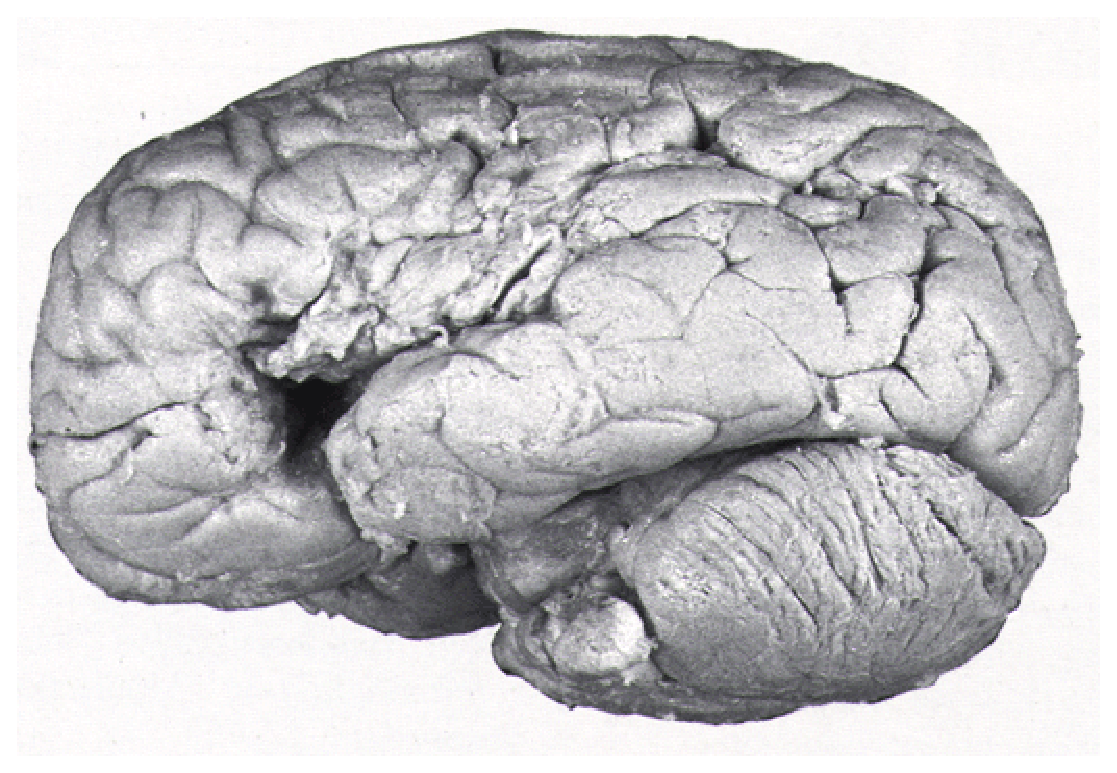
\epsfig{file=include/speech/images/tan.eps, width=0.50\textwidth}

	\caption[Tan's brain]{\textbf{Tan's brain}:
	in 1861 Broca dissected the brain of his patient Leborgned, nicknamed ``Tan''
	due the inability to produce any words other than ``tan''.
	The lesion caused by syphilis in the left cerebral
	hemisphere at the level of Broca's area is clearly visible in the picture.}
	\label{fig:speech:tan}
\end{figure}
% ---------------------------------------------------------------------------- %

At the end of the Ninetieth century, Paul Broca investigated the anatomical
lesions in the left hemisphere that, according to Marc Dax, led to aphasias.
In 1861 Broca dissected the brain of his patient Leborgned, nicknamed ``Tan''
due to the inability to produce any words other than ``tan''.
Broca determined that Tan had a lesion caused by syphilis in the left cerebral
hemisphere, specifically in the ventroposterior region of the frontal lobes
(Broca's area). Figure~\ref{fig:speech:tan} shows a picture of Leborgned's brain
and the lesion at the level of Broca's area.

The early studies on aphasics suggested that in a majority of right and left
handed individuals language processing related to grammar, lexicon, phonemic
assembly and phonetic production depends principally on the left
hemisphere structures.
Also the American Sign Language depends mainly on the left hemisphere, trough it
relies on visuomotor signs rather than auditory speech
signs~\citep{kandel.schwartz.jessel:2000}.

% ---------------------------------------------------------------------------- %
\begin{figure}[htbp]
	\centering
		\epsfig{file=include/speech/images/model.tps, width=0.65\textwidth}

	\caption[Broca's and Wernicke's areas]{\textbf{Broca's and Wernicke's areas.}
	Representation of the simplified Wernicke-Geschwind language processing
	model.
	Broca's area (\textbf{B}) is joined to Wernicke's area by the arcuate
	fasciculus (brown arrow).
	Reproduced from~\citet{kandel.schwartz.jessel:2000}.}
	\label{fig:speech:wg}
\end{figure}
% ---------------------------------------------------------------------------- %

The study of the brain lesions leading to speech disabilities identified two
main cortical areas implied in the processes of speech production and
perception.
The first one, Broca's area, is located on the frontal lateral region, and it
is devolved to the articulation of speech.
The latter one, Wernicke's area, is located in the posterior superior temporal
lobe and is involved in the processing of the acoustic images of speech.
Broca's Area is connected to Wernicke's area by a neural pathway called the 
arcuate fasciculus (Figure~\ref{fig:speech:wg}).
Broca's area comprises BA44 and BA45 and it is subdivided in two main portions:
the anterior \emph{pars triangularis} and the
posterior \emph{pars opercularis}~\citep{kandel.schwartz.jessel:2000}.
Functional evidence suggest that human BA44 contains both speech representation
and motor representation of hand movements, as does area F5 in the macaque 
monkey. 
Those results strongly suggest that human Broca's area is the homologue of
monkey's area F5~\citep{rizzolatti.craighero:2004}.
Neurophysiological investigations reveal that area F5 is agranular while Broca's
area is dysgranular, 
thus suggesting that that a cortical area comparable
in architecture to human area 44 exists in the macaque monkey immediately in 
front of premotor cortical area 6V (inside the inferior arcuate sulcus) and
that it is involved with the orofacial musculature~\citep{petrides.etal:2005}:
\begin{quote}
We suggest that area 44 might have evolved originally as an area exercising 
high-level control over orofacial actions, including those related to 
communicative acts, and that, in the human brain, area 44 eventually also came 
to control certain aspects of the speech act.
\end{quote}
The findings about Broca's and Wernicke's area brought to the development of the
classical Wernicke-Geschwind model of language processing, which is founded on 
three assumptions. 
Firstly, processing is handled by Broca's and Wernicke's areas. 
Secondly, the arcuate fasciculus was thought to be an unidirectional pathway
connecting Wernicke's to Broca's area. 
Lastly, both areas were thought to interact with the polymodal association
cortices \footnote{The association cortices include most of the cerebral
surface of the 
human brain and are largely responsible for the complex processing that goes 
on between the arrival of input in the primary sensory cortices and the 
generation of behavior. 
Inputs to the association cortices include projections from the primary and
secondary sensory and motor cortices, the thalamus, and the brainstem. 
Outputs from the association cortices reach the hippocampus, the basal ganglia
and cerebellum, the thalamus, and other association cortices
\citep{purves.etal:2001}.}.
The Wernicke-Geschwind model provide a useful framework for the classification
of aphasias, although modern studies outstand it in terms of 
complexity\footnote{Recent findings reveal that the role of Broca's and 
Wernicke's areas is not clear as it appears in the Wernicke-Geschwind model.
Moreover, the arcuate  fasciculus is characterized by bidirectional properties
and joins a large set of sensory cortices with prefrontal and premotor cortices.
Lastly, language processing involve higher-order association cortices in the 
left frontal, temporal and parietal 
regions~\citep{kandel.schwartz.jessel:2000}.}.
% ---------------------------------------------------------------------------- %
\subsection{Aphasias}
\label{sec:speech:language:aphasias}
% ---------------------------------------------------------------------------- %
Aphasia is the loss of the ability to produce and/or perceive language correctly
due injuries to specific brain areas. Aphasic patients are normally intelligent
and do not suffer of muscle paralysis.

Broca's aphasia is caused by damage to the frontal lobe of the left hemisphere
of the brain. Subjects with Broca aphasia speak short phrases that require great
effort. 
Subjects with Broca aphasia often have right side paralysis since the injury 
could affect the motor cortex, that is located near by Broca's area.
Subject with Wernicke aphasia do not suffer of paralysis or weakness since the
Wernicke's area is located in the temporal lobe.

Many other types of aphasias have been reported and the classification appears
to be more complex and fine-grained with respect to what is presented in this
Section.
This Section aims to cover the principles of language processing in humans and,
for this reason, just three types of aphasias are discussed.
% ---------------------------------------------------------------------------- %
\subsubsection{Broca aphasia}
\label{sec:speech:language:aphasias:broca}
% ---------------------------------------------------------------------------- %
Broca aphasia is due large frontal lobe lesions involving Broca's area, the
surrounding frontal fields\footnote{BA6, BA8, BA9, BA10 and BA46}, the
underlying white matter, insula, basal ganglia and a small portion of the
anterior superior temporal gyrus. The patient speech is slow and articulation is
impaired. Furthermore, the melodic intonation of speech is
lacking~\citep{kandel.schwartz.jessel:2000}.
If the damage occurred just at the level of BA44 and BA45, the patient develops
a milder aphasia (Broca area aphasia) rather than a true Broca aphasia.
The production of speech is definitely impaired, but aphasics can still
communicate successfully since the selection of words is often correct.
Comprehension is only partial and aphasics loose the ability to repeat complex
sentences spoken by the examiner.
Broca's aphasia is not a production-only deficit. In fact, aphasics cannot
understand complex sentences that rely on complex grammatic structures
(e.g.: recursive sentences). On the other hand, aphasics can infer the meaning 
of simple sentences starting from the meaning of each word.
% ---------------------------------------------------------------------------- %
\subsubsection{Wernicke aphasia}
\label{sec:speech:language:aphasias:wernicke}
% ---------------------------------------------------------------------------- %
Wernicke aphasia is caused by damage to the posterior sector of the left
auditory association cortex (BA22).
In severe cases, lesions extend to the middle temporal gyrus and deep white
matter.
Subjects that suffer of this form of aphasia speak effortless at normal rate 
and the production appears melodic, although they make frequent errors in the 
choice of words and phonemes, leading to unintelligible
words~\citep{kandel.schwartz.jessel:2000}.

Wernicke's area is no longer considered involved in auditory comprehension.
Indeed, the modern view suggest that Wernicke's area constitute the center for 
speech sound processing. 
% ---------------------------------------------------------------------------- %
\subsubsection{Conduction aphasia}
\label{sec:speech:language:aphasias:conduction}
% ---------------------------------------------------------------------------- %
Conduction aphasia results from damage to the left superior temporal gyrus and
the inferior parietal lobe (BA39 and BA40) but the damage may extend to the
primary auditory cortex (BA41 and BA42), the insula and the underlying white
matter. There is no evidence that conduction aphasia is due the damage of the
arcuate fasciculus, although the damage interrupts its projections that connect temporal, parietal, insular and frontal 
cortices~\citep{kandel.schwartz.jessel:2000}.
% ---------------------------------------------------------------------------- %
\section{The articulatory mechanism}
\label{sec:speech:language:mechanism}
The purpose of this Section is to briefly describe the anatomical structures
involved in human speech production (lungs, jaw, lips, hard and soft palate, 
larynx and pharynx, where the vocal folds are located) not paying much
attention to the  phonological aspects of articulation.
The air in the lungs pass trough the pharynx then out trough the oral and the
nasal cavity.
During voiced sounds (vowels) the vocal folds oscillate generating a
quasi-periodic pressure wave. 
In contrast, during the production of unvoiced sounds, the air flow trough the
vocal folds is unobstructed.
The air flow trough the oral cavity is modulated by the position of the lips,
the tongue and the jaw that modulate the deformation of the vocal cavity
resulting in an amplification of attenuation of the different harmonics of the
excitation signal. 
For example, a small constriction of the vocal tract between the tongue and 
the hard palate leads to the production of 
\emph{fricative}\footnote{Fricatives (or spirants):
consonants produced by forcing air trough a narrow channel.} sounds like
\textbf{/s/}.
The rapid release of the air pressure built behind a closure in the oral cavity
leads to high-frequency burst sounds. 
For example, the fast release of the lips cause the emission of the
sound \textbf{/p/}~\citep{blackburn:1996,epstein.etal:2002}.
% ---------------------------------------------------------------------------- %
\subsubsection{The lungs}
Air is pushed in the lungs by the action of different muscles: the
\emph{internal} and the \emph{external intercostals}, the \emph{rectus 
abdominis}, the \emph{external obliques} and the \emph{diaphragm}.
The thoracic cavity can be enlarged by raising the rib cage with the 
external intercostals muscles or by lowering (by contraction) the diaphragm. 
Expiration is a passive process but, during speech, can be modulated by the
expiratory action of the internal intercostal muscles.
If, at the end of an utterance, the intercostals alone cannot produce the
required pressure inside the thoracic cavity, the rectus abdominis and the 
external obliques can push the diaphragm upward 
(Figure~\ref{fig:speech:articulators:lungs}).
% ---------------------------------------------------------------------------- %
\begin{figure}[htbp]
	\centering
		\epsfig{file=include/speech/images/lungs.tps, width=0.30\textwidth}

	\caption[Posterior surface of sternum]{\textbf{Posterior surface of sternum.}
	Reproduced from~\citet{gray:1918}.}	
	\label{fig:speech:articulators:lungs}
\end{figure}
% ---------------------------------------------------------------------------- %

% ---------------------------------------------------------------------------- %
\subsubsection{The jaw}
During speech, the position of the jaw affects the position of the tongue thus
modulating the distance between the tongue and the hard palate.
This distance is involved in the production of
\emph{sibilant}\footnote{Sibilants (or stridents): a subset of fricative
consonants. In addition the tongue is curled lengthwise to direct the air over 
the edge of the teeth.}
consonants such as \textbf{/s/} and \textbf{/z/}.
Furthermore, proper positioning of the jaw plays a fundamental role
in the production of labial consonants.
\comment{(e.g.: \textbf{/p/},
\textbf{/b/}, \textbf{/m/}, \textbf{/f/} and \textbf{/v/})}
Three muscles contribute to jaw closing: the \emph{masseter} elevates and draws
forward the angle of the mandible, the anterior two thirds of
the \emph{temporalis} muscle help the elevation movement and the
\emph{buccinator} pulls back the angle of the mouth and flattens the cheek area
(Figure~\ref{fig:speech:articulators:jaw}).
% ---------------------------------------------------------------------------- %
\begin{figure}
	\centering
	  \subfigure[\label{fig:speech:articulators:jaw:1}]
		{\includegraphics[width=0.35\textwidth]{include/speech/images/jaw_buccinator.tps}}
	  \hspace{0.05\textwidth}
	  \subfigure[\label{fig:speech:articulators:jaw:2}]
		{\includegraphics[width=0.55\textwidth]{include/speech/images/jaw_head.tps}}

	\caption[Muscles of the head, face and neck]{\textbf{Muscles of the head, face and neck.} 
	Reproduced from~\citet{gray:1918}.}	
	\label{fig:speech:articulators:jaw}
\end{figure}
% ---------------------------------------------------------------------------- %

% ---------------------------------------------------------------------------- %
\subsubsection{The lips}
According to~\citet{epstein.etal:2002}, three are the most important movements
of the lips during speech.
The first one is \emph{rounding-spreading}. Rounding occurs when the lips are
drawn together by the action of the \emph{orbicularis oris muscle}
The opposite movement (spreading) occurs when the lips are pulled apart by the
\emph{zygomaticus muscles} (\emph{major} and \emph{minor}), the buccinator and
the \emph{risorius} muscle.
The second movement is \emph{protrusion} and is made protruding the lips to
obtain a longer vocal tract.
The upper lip is controlled by the \emph{levator labii superioris} and by the
zygomaticus minor. On the other hand, the muscles that play a major role in
controlling the lower lip are the \emph{mentalis} and the \emph{depressor
labii oris} (Figure~\ref{fig:speech:articulators:jaw}).
Lastly, the third movement is \emph{compression}, where the lips come together. 
This effect is due the activation of the inferior part or the orbicularis muscle
and the mentalis muscle but can also be achieved raising the jaw.
% ---------------------------------------------------------------------------- %
\subsubsection{The palate}
The soft and hard palate separate the oral cavity from the nasal cavity.
The soft palate is made up by connective tissue and regulates the opening
between the nasopharynx  and the oropharynx.
Specifically, the \emph{tensor palatini muscle} and the \emph{levator palatini
muscle} control the movement of the soft palate.
The hard palate comprises two thirds of the palate and it is made by bone,
as shown in Figure~\ref{fig:speech:articulators:mouth}.
% ---------------------------------------------------------------------------- %
\begin{figure}
	\centering
	  \subfigure[\label{fig:speech:articulators:mouth:1}]
		{\includegraphics[width=0.45\textwidth]{include/speech/images/palate_hardsoft.tps}}
	  \hspace{0.05\textwidth}
	  \subfigure[\label{fig:speech:articulators:mouth:2}]
		{\includegraphics[width=0.35\textwidth]{include/speech/images/mouth_sagittal.tps}}

	\caption[Sagittal view of mouth and palate]{\textbf{Sagittal view of mouth and palate.} 
	Reproduced from~\citet{gray:1918}.}	
	\label{fig:speech:articulators:mouth}
\end{figure}
% ---------------------------------------------------------------------------- %

% ---------------------------------------------------------------------------- %
\subsubsection{The pharynx, the larynx and the vocal folds}
The pharynx is the part of the throat situated posterior to the mouth and nasal
cavity and superior to the esophagus.
The \emph{nasopharynx} is nasal part of the pharynx and it is located behind 
and above the soft palate.
The \emph{oropharynx} constitutes the oral part of the pharynx. It
reaches from the soft palate to the level of the hyoid bone
(Figure~\ref{fig:speech:articulators:larynx}).

% ---------------------------------------------------------------------------- %
\begin{figure}[htbp]
	\centering
		\epsfig{file=include/speech/images/vocalfolds.tps, width=0.45\textwidth}

	\caption[Vocal folds]{\textbf{Vocal folds.}
	Reproduced from~\citet{gray:1918}.}	
	\label{fig:speech:articulators:vocalfolds}
\end{figure}
% ---------------------------------------------------------------------------- %

The vocal folds are located inside the larynx, which is situated just below
where the pharynx splits into the trachea and the esophagus
(Figure~\ref{fig:speech:articulators:vocalfolds}).
In this context, the major movements for speech production are: abducting or
adducting, lengthening or shortening, tensing or relaxing the vocal folds and 
raising or lowering the larynx~\citep{epstein.etal:2002}.
Vocal folds adduction is necessary for speech, while abduction happens
during breathing. The length of the vocal folds modulates the pitch of voiced
sounds while their tension modulates phonation.
The vocal folds are attached to the thyroid cartilage (at the front) and to the 
arytenoid cartilages (at the rear). When those two cartilages move, the vocal
folds increase or decrease their length, vibrating at higher or lower
frequencies thus varying the pitch of the voice. 
% ---------------------------------------------------------------------------- %
\begin{figure}
	\centering
	  \subfigure[\label{fig:speech:articulators:larynx:1}]
		{\includegraphics[width=0.40\textwidth]{include/speech/images/larynx_frontal.tps}}
	  \hspace{0.05\textwidth}
	  \subfigure[\label{fig:speech:articulators:larynx:2}]
		{\includegraphics[width=0.45\textwidth]{include/speech/images/larynx_behind.tps}}

	\caption[Antero-lateral and posterior view of the larynx]{\textbf{Antero-lateral and posterior view of the larynx} 
	Reproduced from~\citet{gray:1918}.}	
	\label{fig:speech:articulators:larynx}
\end{figure}
% ---------------------------------------------------------------------------- %

% ---------------------------------------------------------------------------- %
\subsubsection{The tongue}
The tongue is made of skeletal muscles and its \emph{dorsum}\footnote{Dorsum:
upper surface} can be divided in two parts.
The first one is the \emph{oral part} and it comprises the first two thirds of
the tongue. The \emph{pharingeal part} faces back to the oropharynx.
Two groups of muscles play a crucial role for tongue movement:
the \emph{extrinsic muscles}, that originate
outside the tongue and connect it with other structures 
and the \emph{intrinsic muscles}, that lie within the tongue.
Those two groups of muscles are described in the next two paragraphs.

The \emph{genioglossus muscle} forms the bulk of the inferior part of the
tongue. It originates from the mandible and its activation pulls the tongue 
forwards.
On the other hand, the \emph{styloglossus muscle} elevates and pulls the tongue
backwards, connecting the tongue with the styloid process.
The \emph{palatoglossus muscle} can assist the action of the styloglossus.
The \emph{hyoglossus muscle} pulls the tongue downwards while the 
\emph{mylohyoid muscle} raises its body.
The mylohyoid muscle forms the floor of the mouth and it is involved in the
elevation of the hyoid bone, and consequently of the larynx.
% ---------------------------------------------------------------------------- %
\begin{figure}
	\centering
	  \subfigure[\label{fig:speech:articulators:tongue:4}]
		{\includegraphics[width=0.30\textwidth]{include/speech/images/tongue_4.tps}}
	  \subfigure[\label{fig:speech:articulators:tongue:3}]
		{\includegraphics[width=0.35\textwidth]{include/speech/images/tongue_3.tps}}

	\caption[Posterior and lateral view of the tongue muscles]{\textbf{Posterior (intrinsic muscles) and lateral view of the tongue (extrinsic muscles).} 
	Reproduced from~\citet{gray:1918}.}	
	\label{fig:speech:articulators:tongue:b}
\end{figure}
% ---------------------------------------------------------------------------- %


Four are the intrinsic muscles that run along the length of the tongue.
The \emph{superior longitudinal muscle} is located under the dorsum of the
tongue and controls the elevation, the deviation and the retraction of the apex.
The \emph{inferior longitudinal muscle} is joined with the styloglossus muscle
and is located on the inferior sides of the tongue.
The \emph{verticalis muscle} and the \emph{transversus muscle} are located in
the body of the tongue. The first one is connected to the superior and the
inferior longitudinal muscles while the latter is attached to the mucous
membrane.
% ---------------------------------------------------------------------------- %
\begin{figure}
	\centering
	  \subfigure[\label{fig:speech:articulators:tongue:1}]
		{\includegraphics[width=0.35\textwidth]{include/speech/images/tongue_1.tps}}
	  \subfigure[\label{fig:speech:articulators:tongue:2}]
		{\includegraphics[width=0.55\textwidth]{include/speech/images/tongue_2.tps}}

	\caption[Oral cavity and coronal section of the tongue]{\textbf{Anterior view of the oral cavity and coronal section of the tongue (intrinsic muscles).} 
	Reproduced from~\citet{gray:1918}.}	
	\label{fig:speech:articulators:tongue:a}
\end{figure}
% ---------------------------------------------------------------------------- %

% ---------------------------------------------------------------------------- %
\section{Motor role of Broca's area in speech}
\label{sec:speech:mirror}
% ---------------------------------------------------------------------------- %
According to the motor theory of speech
perception~\citep{liberman.mattingly:1985}, the objects of speech are the 
phonetic gestures of the speaker (e.g.: tongue backing, lip rounding, jaw
raising).
Those actions of speech are intended as the elementary events of speech
production and perception. 
According to the theoretical framework proposed by Liberman and Mattingly, these
actions are represented in the brain as invariant motor commands 
and, during vocalization, are translated in significant configurations of the
articulators (Section~\ref{sec:speech:language:mechanism}).
Furthermore, if speech perception and speech production share the same set of
invariants, they must be strictly coupled at the brain level.
According to the authors, this link is not built by learning: on the contrary, 
it is innately specified and requires epigenetic development to be achieved.

\citet{fadiga.craighero.etal:2002} found that during speech listening there is
an increase of MEPs recorded from the tongue muscles, demonstrating that
listening activates brain areas involved in motor control.
The experimenters stimulated the left motor representation of the tongue by the
means of TMS while subjects were passively listening to Italian words and
pseudo-words that involve a certain degree of tongue mobilization.
The verbal stimuli used in the experiment could be grouped in two main sets.
The first set groups stimuli characterized by an high degree of tongue
mobilization such as words /birra/, /carro/ and pseudo-words /berro/,
/marro/\footnote{/bi\textbf{rr}a/, /ca\textbf{rr}o/, 
/be\textbf{rr}o/ and /ma\textbf{rr}o/: labiodental fricative
consonant~\textbf{/rr/}.}.
The latter set contained stimuli characterized by a lower degree of tongue
mobilization such as 
words /baffo/, /beffa/ and pseudo-words /ciffo/,
and /ceffa/\footnote{/ba\textbf{ff}o/, /be\textbf{ff}a/, 
/ci\textbf{ff}o/ and /ce\textbf{ff}a/: lingua-palatal fricative
consonant~\textbf{/ff/}.}.
The MEPs evoked by TMS stimulation reached higher amplitudes when the subjects
were listening to /\textbf{rr}/ stimuli. 
Furthermore, words did evoke an higher response than pseudo-words.
The presented results suggest that speech listening
activates precise motor areas with ah high degree of specificity in
discriminating words and non-words sounds.
The work by \citep{fadiga.craighero.etal:2002} does not prove that the
theoretical framework provided by Liberman and Mattingly matches the way the
human brain handles speech perception. On the other hand, the
acoustic/motor resonance resembles the visual/motor resonance typical of the
visuomotor mirror neurons.
According to~\citet{liberman:1993}\footnote{This quotation can be also found at
the real beginning of \citet{rizzolatti.arbib:1998}.}:
\begin{quote}
In all communication, sender and receiver must be bound by a common
understanding about what counts; what counts for the sender must count for the
receiver, else communication does not occur. Moreover the process of production
and perception must somehow be linked; their representation must, at some point,
be the same.
\end{quote}
Two are the main concepts condensed in the quotation. 
Firstly, both the sender and the receiver must share a common repertoire of
speech-oriented motor actions.
The results of the previous experiment show that the motor system resonates
during speech listening the same way it resonates during observation of motor 
actions.
Secondly, speech production and speech perception must be linked abilities. 
The mirror system links action production and action perception at the very low
level of single visuomotor (or audiomotor) neurons.
The presented considerations, as said before, do not prove Liberman's framework,
but reinforce the idea that speech abilities in human may have evolved from
well-founded motor abilities in primates.
\comment{Eventually, Roy etal}

According to~\citet{rizzolatti.arbib:1998}, language evolved from gestural
communication, an ability where the mirror system plays a fundamental role.
In fact, monkey's mirror neurons discharge both during the observation and the
execution of a specific transitive action.
Furthermore, a subset of F5 mirror neurons discharge during the
observation of mouth movements for communication and
eating~\citep{ferrari.etal:2003}. 
Mirror neurons do not embed just visuomotor properties; in fact, audio-motor
mirror neurons discharge both when an action is made by the monkey and when the
monkey ears the action-specific sound~\citep{kohler.etal:2002}.
In a broader perspective the mirror system creates a link between the actor and 
the observer.
%integrating motor proprioception (?information, ma sarebbe una
%ripetizione?) with other kinds of sensory information.
In this context, the mirror system acts as a neural circuit that allows
unconscious processing of the perceived motor actions.

Broca's area is involved in language processing in both the cases of production
and perception~(Section~\ref{sec:speech:language:wg}).
Recent findings demonstrate that Broca's area becomes active
during action observation~(Section~\ref{sec:actions:human}), thus extending its
evolutionary importance.
As said before,~\citet{rizzolatti.arbib:1998} hypothesize that
speech originated from ancient gestural communication abilities by supporting
the idea that primates mainly used oro-facial gestures for one-to-one 
communication. 
In fact, oro-facial expressions combined with brachio-manual gestures
could have enhanced communications since the sender could reinforce its message
providing an higher level of description making transitive and intransitive
gestures.
Furthermore, oro-facial communication in primates does not embed the same
combinational properties that are common to brachio-manual gestures.
According to ~\citet{rizzolatti.arbib:1998}, the primitive use of vocalization
in
primates was to transmit emotionally relevant messages.
%\footnote{This ability is mediated by brain medial 
%areas~\citep{kandel.schwartz.jessel:2000}.}
When a strong link was estabilished between the brachio-manual and the
oro-facial 
communication systems, the control of vocalization gained further importance
since the early utterances did need to be repeatable in order to be imitated.
For this reason, the old control system was inadequate.
A ``Broca's area F5-like precursor'' with mirror properties may have been the
right choice for the control of the novel oro-laryngeal movements.
Manual gestures gradually lost their primitive importance in communication, but 
are still widely used in to enrich the message transmitted by the sender.
A recent study, here presented, investigated the role of Broca's area in both
the fields of speech and motor actions.

In subjects with large lesions involving Broca's area, speech production and
speech perception are impaired, although this is valid just for complex
sentences, since single words perception is not totally
impaired.
In order to verify this claim, 
\citet{fadiga.etal:PRESS} administered single TMS pulses in correspondence of
BA44 while subjects where performing a \emph{phonological 
priming}\footnote{Phonological priming: a target word preceded by a prime that
share with the target the last syllable is recognized faster than the word by 
itself (e.g.: roccia, doccia; palla, stalla). The facilitation in recognition is
referred as \emph{phonological priming effect}.} task. 
Subjects where asked to listen to pairs of stimuli, both words and pseudo-words 
(e.g.: W-W, W-PW, W-PW and PW-PW). 
For certain pairs, the target and the prime did share the last syllable (priming
effect). In some trials, a single TMS pulse was administered between the prime
and the target.
In trials where BA44 functionality was not blocked by TMS pulses, the
experimenters found that the lexical content is crucial for the emergence of the
priming effect\footnote{1. The phonological priming effect appeared 
for stimuli such as W-W, W-PW, PW-W. 
2. Furthermore, no priming effect was present for PW-PW pairs.
3. Lastly, the subject response was faster during W-W and W-PW pairs.} (e.g.:
priming effect for pairs W-W, PW-W and W-PW; no priming effect for PW-PW pairs).
According to the authors, this last result demonstrate that the phonological
priming effect is not a phonological-only effect, since it can not be
observed when the prime-target pair does not contain lexical entries.
During TMS trials, the priming effect was suppressed for the W-PW pairs thus
confirming that Broca's area is not involved in phonological processing of the
stimuli. 
In particular, Broca's area may be involved in supramodal syntactic processing.
%provides access to the lexical content of the
%prime 

In order to verify this very last claim, the authors point out that subjects
suffering of Broca aphasia should also suffer of more broad motor
deficits.
Videos representing biological actions (e.g.: hand grasping a bottle, man
opening a door) and non-biological moving objects (e.g.: a bike falling on the 
ground) have been shown to agrammatic patients impaired by Broca
aphasia and to healthy subjects\footnote{Unpublished results (Fazio et al.) 
described in~\citet{fadiga.etal:PRESS}}.
Later on, the patients were asked to place in the correct temporal order four
frames extracted from the previously observed in the videos (e.g.: man
approaching the door, man moving the hand toward the door handle, man acting
on the handle, man opening the door).
The results demonstrate that aphasics were slower than the
control group. Moreover, aphasics perform better in terms of accuracy on 
non-biological sequences, while the opposite is true for the control group.



% ---------------------------------------------------------------------------- %
\section{The Linguometer instrumentation}

\label{ch:linguometer:instrumentation}

%\label{ch:linguometer}
%Simultaneous acquisition of phono-articulatory features
% ---------------------------------------------------------------------------- %
We describe the work done for the CONTACT
Project assembling and running an experimental setup for the simultaneous 
acquisition of phono-articulatory features, the ``Linguometer''.
The data recorded with the Linguometer will be used to build an audio-motor map 
that will allow a robot to recognize at least a small subset of words.
If the hypothesis that speech relies on invariant motor commands is correct, 
the articulatory features recorded with the Linguometer should allow the
model to outperform similar models based only on the phonetic features.
The performance of the model will be tested in two cases.
In the first case training and testing will be done using just phonetic
features. In the second case, both phonetic and articulatory (motor) features
will be used during training, while testing will still rely on just the acoustic
features.
The idea is to build an audio-motor map (AMM), that will translate the acoustic 
features to motor features. 
%The motor space, that is the kinesthetic representation of speech, should be
%simpler than the corresponding phonetic space (less degrees of freedom, is it
%correct Paul?) and, according to Liberman's theoretical framework and the
%studies on the mirror system, should be characterized by some degree of
%invariance (again, does it make sense?).
The motor space, that is the kinesthetic representation of speech, constitutes
a better space in which to perform learning and classification.
In fact, according to Liberman's theoretical framework and the
studies on the mirror system, the motor representation of speech should be 
characterized by some degree of invariance.

In previous work,
\citet{metta.etal:2006} developed a biologically-inspired Bayesian model of
the mirror system.
The authors demonstrated that kinesthetic and tactile information associated to
a certain hand action can simplify the recognition of the same action when the
only information available is the visual one.
Moreover, the experimenters were interested in determining if the artificial
model
of the mirror system was effectively able to learn the motor invariance common
to different grasping types.
In order to feed the appropriate kinesthetic information to the system, a data
glove (CyberGlove by Immersion) with 22 sensors.
A magnetic tracker recorded the position and the orientation of the hand with
respect to a reference frame.
Tactile features were provided by two touch sensors. The actions performed by
the subjects were recorded using a pair of CCD cameras, thus providing the
visual information required by the visuomotor model. 
The six recorded subjects were asked to grasp three different objects 
(e.g.: a small glass ball, a rectangular solid, and a large sphere) making three
different grasping actions (e.g.: precision grasping, power grasp and power
grasp).
The visual features of the grasping actions were recorded from 12 different
locations. Moreover, each action was performed 5 times.
Once the data was recorded using the setup here described, the model was
trained and tested in two cases. Classification rate of the perceived actions is
used to describe the performance of the model.
In the first case, the model was trained and tested only using visual
features.
In the latter, the model was trained using all the available visuo-motor 
features and tested by feeding to the system only the visual
information.
The authors report a classification rate of $97\%$ (training set) and $80\%$
(test set) for the first case. 
When the model was fed using visuo-motor features during training, its
performance was higher in the test set ($98\%$ training set, $97\%$ test 
set), demonstrating that, at least in the case of the described model, the
motor information plays a crucial role in the action recognition process.
%In fact, when available, the visuo-motor features were used to build a
%more accurate visuo-motor inverse model (or VMM, visuo-motor inverse map)
%than in the plain visual case.
In fact, when available, the visuo-motor features were used to build a
visuo-motor map (VMM) that mapped the visual features onto the motor space.

Measuring the activity of the articulators (the tongue, the larynx, the lips and
the jaw) during speech is not trivial. 
Firstly, the articulators are fairly inaccessible.
Secondly, no Linguometer-like instrumentation is available on the market.
Lastly, speech production should not be affected by the recording devices.
Taking these three points into account, the Linguometer has been assembled 
interconnecting different instruments, building custom devices, and finally
writing the required software (e.g.: setup-control, stimuli presentation, data
handling, data processing, signal synchronization and segmentation).
Once the Linguometer was finally been built, a total of nine
experiments have been run (Section~\ref{ch:experiments}) and the data has been
processed (Section~\ref{ch:results}).\\

This section describes how the Linguometer has been built, using a bottom-up
approach. 
Firstly, the instrumentation on which the Linguometer is based is briefly
described, in terms of both principles and implementation

%(Section~\ref{ch:linguometer:instrumentation}).
%(to be continued). 
% ---------------------------------------------------------------------------- %
%\subsection{Instrumentation}
% ---------------------------------------------------------------------------- %
The Linguometer consists of ``a constellation of hardware and
software''\footnote{CONTACT Annex I - ``Description of Work'',
March 2005} that allows the simultaneous recording of acoustic and articulatory
data.
It is made up of several interconnected devices; some of those are 
synchronized in hardware, while the remaining rely on post-processing
synchronization.
The devices and the recording room were made available by the CRIL 
laboratory\footnote{CRIL: Centro di Ricerca Interdisciplinare sul Linguaggio 
(Interdisciplinary Language Research Center).
Homepage: http://www.cril.unile.it.},
where the Linguometer has been built during the period that spans
from August 2006 to January 2007.\\
This Section aims to describe how the instrumentation works and why it is
important for the recordings required by the CONTACT Project.
%Few technical issues are presented here, the building blocks the
%Linguometer relies on are better discussed in
%Section~\ref{ch:linguometer:architecture}.
Firstly the author describes the recording devices that characterize the
Linguometer (Section~\ref{ch:linguometer:instrumentation}).
Secondly, the Linguometer's architecture is discussed, mainly focusing onto the
synchronization topic (Section~\ref{ch:linguometer:architecture}).
Lastly, the author presents and discusses few technical issues emerged during
the integration process (Section~\ref{ch:linguometer:technical}).
% ---------------------------------------------------------------------------- %
\subsection{Electromagnetic articulograph}
\label{sec:linguometer:instrumentation:ag}
% ---------------------------------------------------------------------------- %
An electromagnetic articulograph (EMA) was used to track the movements of a set
of sensors glued on the tongue, on the lips, on the front teeth and on 
a pair of glasses, as it is shown in Figure~\ref{fig:experiments:map}.
%(for head-movement compensation).
The pictures in Figure~\ref{fig:linguometer:ag:tongue} show how the sensors are
positioned onto the tongue to track tongue movements during speech production.
The device used for the Linguometer is an ``Articulograph AG500'' made by
Carstens Medizinelektronik GmbH, G\"ottingen, Germany.

The AG500 articulograph could determine the three-dimensional spatial 
arrangement (Cartesian coordinates $x$, $y$ and $z$) and the orientation
(spherical coordinates azimuth $\theta$ and elevation $\rho$)
of up to twelve 
directionally sensitive magnetic field sensors at a sampling frequency of 200Hz.
The measuring sensors are single axis coils.
Six reference coils, arranged to form a three-dimensional frame of
reference, emit six magnetic fields at different frequencies:
7500, 8750, 10000, 11250, 12500 and 13750 Hz.
The alternating current induced in the sensor by the alternating magnetic fiels
of the reference coils is measured.
The measuring device distinguishes and separates the alternating voltages
induced by the individual alternating magnetic fields by their 
frequencies.
During a recording session the separated and digitized current signals are
sent in real-time to the AG500 control PC (using an Ethernet connection).
Software provided by Carstens Medizinelektronik GmbH stores the current values
on the hard drive of the control PC, making those available for the spatial 
arrangement determination process.
The main idea behind the spatial determination process is that the distance 
between the sensors and the reference coils is determined from the
absolute values of the induced currents. 
The position vector and the direction vector of a sensor can then be calculated
starting from the six field equations of the reference coils, using an iterative
method~\citep{zierdt.carstens:1993}.

% ---------------------------------------------------------------------------- %
\begin{figure}
	\centering
	  \subfigure[\label{fig:linguometer:ag:intro:cube1}]
		{\includegraphics[width=0.45\textwidth]{include/linguometer/images/ag_cube1.tps}}
		\hspace{0.05\textwidth}
	  \subfigure[\label{fig:linguometer:ag:intro:cube2}]
		{\includegraphics[width=0.45\textwidth]{include/linguometer/images/ag_cube2.tps}}

	\subfigure[\label{fig:linguometer:ag:intro:magazine}]
		{\includegraphics[width=0.45\textwidth]{include/linguometer/images/ag_magazine.tps}}
		\hspace{0.05\textwidth}
	\subfigure[\label{fig:linguometer:ag:intro:circal}]
		{\includegraphics[width=0.45\textwidth]{include/linguometer/images/ag_circal.tps}}

	\caption[Articulograph AG500]{\textbf{Articulograph AG500: EMA-Cube, magazines and Circal}:
	(a) Prof. M. Grimaldi, CRIL evaluates the correct posture required by the
	subjects when recording using the articulograph AG500.
	Five out of the six reference coils are visible: two red, two green and a
	blue one. The sixth sensor (blue) is located just behind Prof. Grimaldi's
	head, on the top of the EMA-Cube.
	Just at the top of Prof. M. Grimaldi's head, the Circal mounting slot is
	visible (white structure).
	(b) Prof. M. Grimaldi during an experiment (some sensor wires are visible).
	(c) A magazine with four sensors mounted. 
	(d) The magazine attached to the Circal calibration device.
	Photos courtesy of Prof. M. Grimaldi and Dr. B. Gili Fivela, CRIL.}
	\label{fig:linguometer:ag:intro}
\end{figure}
% ---------------------------------------------------------------------------- %

The AG500 articulograph is sensitive to electrically or magnetically conductive
objects. 
In fact, if one or more of those objects are placed nearby the transmitter (or
reference) coils, the generated magnetic fields are distorted.
If the interfering object moves, a time-varying distortion affects the
magnetic field.
On the other hand, if the interfering object does not move, the
distortion is constant in time (static distortion). 
Furthermore, in the second case, the interference can be
corrected since the resulting error depends on the distance between the
reference coils and the conductive object.

Before each recording session, the AG500 is calibrated in order to
tune the six field equations that map current values to position/orientation
values.
Furthermore, calibration is useful to compensate for the possible static
distortions. 
The twelve sensors (or less, it depends on how many sensors the investigation 
requires) are placed in appropriate magazines mounted on a dish (Circal) inside
the  frame of reference (EMA-Cube).
Figure~\ref{fig:linguometer:ag:intro} shows the previously mentioned devices.
A program developed by Carstens Medizinelektronik GmbH rotates the Circal using an
electrical motor (located on top of the EMA-Cube) moving each sensor until it 
reaches a well known position.
Once the target position is reached, the corresponding current amplitudes  
are acquired. The control PC then calculates the calibration factors that are
necessary to convert the currents acquired during an
investigation in consistent positions.
A synchronization device (Sybox Opto-4) is connected to the articulograph
AG500 and
%This device is used by the Linguometer to allow the synchronized acquisition of
%phono-articulatory gestures.
it is heavily used by the Linguometer in order to allow the synchronized 
acquisition of phono-articulatory gestures.
For this reason, a few words should be spent describing how this device works.

Both the Sybox Opto-4 device and a microphone are connected to the Line-In jack
of the control PC sound card (left and right channel respectively).
After an investigation is started, the recording software asks the AG500 to
start sending data and waits for the synchronization signal to appear on the
left-channel of the Line-In connector.
When the synchronization signal is detected, the acquisition software starts
recording both the speech data and the amplitudes data.
A ``low enough'' delay affects the synchronized signals, although its value is
unpredictable and not constant (Bahne Cartsens, personal  communication. 
November 2006).
Cartsens Medizinelektronik GmbH does not provide the source code of the AG500
software (although the Sybox-Opto4 schematic is available).
For this reason, it has not been possible to measure or to estimate the delay
affecting the synchronization, and it will be considered negligible from now on.

% ---------------------------------------------------------------------------- %
\begin{figure}
	\centering
	  \subfigure[\label{fig:linguometer:ag:tongue:f}]
		{\includegraphics[width=0.45\textwidth]{include/linguometer/images/ag_tongue_f.tps}}
		\hspace{0.05\textwidth}
	  \subfigure[\label{fig:linguometer:ag:tongue:m}]
		{\includegraphics[width=0.45\textwidth]{include/linguometer/images/ag_tongue_m.tps}}

	\caption[Articulograph sensors glued on the tongue]{\textbf{Articulograph sensors glued on the tongue}:
	(a) A female subject and (b) a male subject with dorsal and coronal articulograph
	AG500 sensors glued on the tongue. The female subject also has sensors glued
	on the lips and on the upper and lower incisive teeth.
	The reader may find Figure~\ref{fig:experiments:map} useful to better
	understand how the sensors are positioned.}
	\label{fig:linguometer:ag:tongue}
\end{figure}
% ---------------------------------------------------------------------------- %

Once the amplitudes have been recorded, positions can be calculated using the
Cartsens Medizinelektronik GmbH software or the open source TAPADM ToolBox by A.
Zeirdt\footnote{TAPADM homepage:
http://www.phonetik.uni-muenchen.de/\~{}andi/EMAPage/}.
Furthermore, since the subject's head is not constraint during the
investigation, three sensors are used to track head movement and then to
compensate for it.
Moreover, the sensors do need to be kept close to the geometrical center of the
frame of reference.
%center of mass. 
Particularly, Carstens Medizinelektronik GmbH recommends to keep the sensors
inside the 15 cm diameter spherical volume that shares its geometrical center 
with the geometrical center of the frame of reference.
% ---------------------------------------------------------------------------- %
\subsection{Ultrasound system}
\label{sec:linguometer:instrumentation:us}
% ---------------------------------------------------------------------------- %
Modulating the shape of the vocal tract, the tongue plays a critical role in
articulation.
Being positioned deep in the oral cavity, the tongue is a fairly inaccessible 
articulator and requires measuring devices to be inserted inside the mouth. 
Tongue recording for the CONTACT Project took place by gluing a few AG500
sensors on
the tongue and recording tongue motion on the sagittal plane using the Toshiba
Aplio XV Ultrasound System provided with a low frequency convex transducer by
Toshiba, positioned submentally.
Ultrasound investigation of the tongue motion is both non-invasive and non
obtrusive, thus non affecting speech production.
Furthermore, ultrasound images provide the full profile of the tongue
dorsum, although the apex and the radix are often occluded during speech
production
by the jaw and by the hyoid bone respectively. 
According to~\citet{stone:2005}, the acoustic shadows of the hyoid bone can be
used to detect swallowing events.
On the other hand, generally no more than 1 cm of the tongue apex is obscured
by the jaw shadow.

Medical sonography uses high frequency (2-14 MHz) sound waves emitted from a
piezoelectric crystal that produces an image by using the reflective properties
of sound waves.
Piezoelectric crystals undergo a change in size when a voltage is applied.
If the voltage is alternating, the crystal oscillate at high frequency,
producing high frequency sound waves.
Piezoelectric crystals can also be used as ultrasound waves detectors. 
In fact, if a force is applied to a crystal, it generates a voltage.
The ultrasound transducer is equipped with a mono-dimensional array of
piezoelectric transducers, multiplexed in time so that only one crystal emits
sound waves in a given time interval. Immediately after the crystal emits the
pressure wave, all the remaining crystals are used to convert the received 
echoes to voltage values. Voltage values are then processed and the image
is reconstructed.
In order to generate pressure waves, the crystals are heated at high 
temperature so that the molecules they are made of are magnetically aligned  
by the means of dipolar molecular alignment.
When a voltage is applied to the crystals, the molecules first twist in one
direction increasing the crystals' thickness, then in the reverse direction
thus decreasing the thickness~\citep{stone:2005}.
If the applied voltage is alternating, this change in 
thickness produces cyclic sound pressure waves.
The thickness of the crystals determine the resonant frequency of the crystals
themselves.
Moreover, the higher the resonant frequency is, the shorter the wavelength is,
and short wavelengths are important to increase the spatial resolution of the
transducer (\emph{ibid}).

% ---------------------------------------------------------------------------- %
\begin{figure}
	\centering
	  \subfigure[\label{fig:linguometer:us:constraints:f}]
		{\includegraphics[width=0.45\textwidth]{include/linguometer/images/us_larynx_f.tps}}
		\hspace{0.05\textwidth}
	  \subfigure[\label{fig:linguometer:us:constraints:m}]
		{\includegraphics[width=0.45\textwidth]{include/linguometer/images/us_larynx_m.tps}}

	\caption[Ultrasound transducer constraints]{\textbf{Ultrasound transducer constraints}:
	(a) A female subject and (b) a male subject during linguometer recordings.
	The ultrasound probe is placed submentally. The black strap hold the
	laryngograph sensors in fixed position.
	In the specific case of the male subject, the ultrasound transducer touches
	the larynx.}
	\label{fig:linguometer:us:constraints}
\end{figure}
% ---------------------------------------------------------------------------- %

When an ultrasound wave reaches an interface between materials with different
impedance properties, it is reflected. Large density gradients create a strong
echo (e.g.: tissue/air and tissue/bone interfaces) while low density gradients
bring to weak echoes (e.g.: tissue/water and tissue/tissue interfaces).
Figure~\ref{fig:linguometer:us:frame} shows a frame grabbed from an ultrasound
investigation of tongue motion.
The brightest area in the image is the subject's tongue. The brighter the
pixel is, the higher the density gradient is, thus the acquired echoes.
Tongue lamina is clearly visible since a great density gradient exists between
the muscle tissue/air interface.
The same happens for the lower tongue surface.
The hard palate, the hyoid bone and the jaw are not visible since they adsorb
the sound waves, and thus do not produce echoes. 
At the beginning of this Section, it has been said that the tongue and the
palate play a critical role in articulation, since the they modulate the shape
of the vocal tract.
Due to the facts here described, acquiring the palate's profile during the
experiments is not possible, and for this reason the subjects' palates were
recorded off-line, as better discussed in
Section~\ref{sec:experiments:recording}.

While experimenting with tongue recordings, it appeared clear that not all
tongues are suitable for ultrasound investigation during speech production 
tasks.
Furthermore, similar and more detailed conclusions are reported
by~\citet{stone:2005}.
Firstly, female subjects appear to be better candidates for speech production
investigation. Women often image better than men, probably because the tongues
of men are thicker and fatter (fat tissue scatters sound).
Furthermore, men do have a bigger larynx that protrudes from the neck. This
anatomical difference plays a crucial role in speech production recordings,
because the ultrasound transducer is placed submentally and when the larynx
moves, it touches the transducer. 
This mechanical contact produces pain and higher swallowing rates in the
male subjects and made male recordings with the Linguometer quite impractical 
(Fig.~\ref{fig:linguometer:us:constraints}).
Female subjects also have smoother tongues thus producing higher-quality
gradients in the image.
Furthermore, subjects with high salivation often provide better results.
According to~\citet{stone:2005}, the saliva forms a thin film around the tongue,
thus becoming smoother and acting as a better reflector.
Although high salivation provides better ultrasound images, the large amount of
saliva easily wears out the glue used to attach the articulograph sensors to the
tongue. For this reason, subjects with high salivation were not
recorded~(Section~\ref{ch:experiments}).

% ---------------------------------------------------------------------------- %
\begin{figure}
	\centering
	  \subfigure[\label{fig:linguometer:us:intro:full}]
		{\includegraphics[width=0.45\textwidth]{include/linguometer/images/us_full.tps}}
		\hspace{0.05\textwidth}
	  \subfigure[\label{fig:linguometer:us:intro:probe}]
		{\includegraphics[width=0.45\textwidth]{include/linguometer/images/us_probe.tps}}

	\caption[Ultrasound System Toshiba Aplio XV]{\textbf{Ultrasound System Toshiba Aplio XV}:
	(a) The Toshiba Aplio XV Ultrasound System. (b) The convex transducer used for the 
	recordings.}
	\label{fig:linguometer:us:intro}
\end{figure}
% ---------------------------------------------------------------------------- %

Figure~\ref{fig:linguometer:us:intro:full} shows the Toshiba Aplio XV ultrasound
system while~\ref{fig:linguometer:us:intro:probe} shows the convex transducer 
used for the Linguometer recordings.
Figure~\ref{fig:linguometer:us:frame} shows a frame grabbed from the
Toshiba Aplio XV system using an acquisition card attached to the S-Video
Aplio XV video output.
The Toshiba Aplio XV system was shipped with a RAW frame acquisition plug-in
that
allows us to acquire a maximum of 5 seconds of RAW frames, independently from
the acquisition frame rate and the frame resolution.
A RAW frame is intended to be the reconstructed tongue image without any
processing applied.
The acquired sequences are temporarily accumulated in a hardware buffer until
the maximum capacity of the buffer is reached. 
Once it is full, the buffer needs to be emptied saving the RAW data on the 
Aplio XV internal hard drive, shared on the network via the SMB/CIFS network
protocol\footnote{SMB/CIFS: Microsoft standard resource exchange protocol.}.

The RAW plug-in was initially designed by Toshiba for heart investigations, and
for this reason the maximum length of a RAW acquisition was limited to 5
seconds,
probably enough for heart disease studies.
%Moreover, the plug-in did require an experimenter to be used since no automated
%recording procedure is implemented in the plug-in itself.
Moreover, using the plug-in is laborious and time-consuming since no automated 
recording procedure is implemented in the plug-in itself, thus an experimenter
is required to handle the RAW recordings.
For those reasons, the RAW plug-in was dropped, and the S-Video output was
recorded. 
% ---------------------------------------------------------------------------- %
\begin{figure}[htbp]
	\centering
	\epsfig{file=include/linguometer/images/us_frame.tps, width=0.65\textwidth}
	\caption[Ultrasound System video frame]{\textbf{Ultrasound System video frame}:
	A frame grabbed from the S-Video connector. It shows the tongue (resting
	position) of a 25
	years old female subject and the tongue recording convention used for the
	linguometer (sagittal plane, apex on the right, dorsum on the top).}
	\label{fig:linguometer:us:frame}
\end{figure}
% ---------------------------------------------------------------------------- %

Surely the S-Video output does not ensure an image quality comparable with the
RAW data image quality, but consistently simplifies the recording work flow.
A non trivial problem arises recording the S-Video stream. In fact, the 
Toshiba Aplio XV system is a closed source device intended for clinical use 
and probably the image reconstruction does not happen in real-time. 
Toshiba Medical System Europe did not provide enough details about the
processing the reconstructed frames undergo before visualization on the monitor
or presentation on the S-Video connector. 
Frame persistence\footnote{Frame persistence: a technique used to enhance the
quality of a video stream by averaging each frame with few surrounding ones.} 
and many other filters have been disabled in
order to record frames ``corrupted'' by the smallest possible amount of 
post-processing operations.
Moreover, no details were provided about the delays characteristic of the Aplio
XV system.
%All those issues are discussed in Section REF HERE.
% ---------------------------------------------------------------------------- %
\subsection{Laryngograph}
\label{ch:linguometer:instrumentation:lg}
% ---------------------------------------------------------------------------- %
Electroglottography is a technique used to register laryngeal behavior measuring
the change in electrical impedance across the throat during speech production.
The EGG device used for the Linguometer is a ``Laryngograph Microprocessor`` by
Laryngograph Ltd, London, United Kingdom. 
% ---------------------------------------------------------------------------- %
\begin{figure}
	\centering
	  \subfigure[\label{fig:linguometer:lg:intro:front}]
		{\includegraphics[width=0.45\textwidth]{include/linguometer/images/lg_front.tps}}
	  \hspace{0.05\textwidth}
	  \subfigure[\label{fig:linguometer:lg:intro:rear}]
		{\includegraphics[width=0.45\textwidth]{include/linguometer/images/lg_rear.tps}}
	  
	  \subfigure[\label{fig:linguometer:lg:intro:sensors}]
		{\includegraphics[width=0.45\textwidth]{include/linguometer/images/lg_sensors.tps}}
	  \hspace{0.05\textwidth}
	  \subfigure[\label{fig:linguometer:lg:intro:strap}]
		{\includegraphics[width=0.45\textwidth]{include/linguometer/images/lg_strap.tps}}

	\caption[Laryngograph MicroProcessor]{\textbf{Laryngograph MicroProcessor}:
	Front (a) and rear (b) view of the Laryngograph MicroProcessor. The USB
	connector, the microphone and the EGG electrodes connectors are
	shown. (c) EGG electrodes, available in three different sizes. (d) A subject
	wears the EGG electrodes, kept in fixed position using the visible black
	flexible band.
	Photos (a), (b) and (c) courtesy of Prof. M. Grimaldi and Phd. B. Gili Fivela, CRIL.}
	\label{fig:linguometer:lg:intro}
\end{figure}
% ---------------------------------------------------------------------------- %


An high frequency current, small both in voltage and amperage, passes between
two electrodes situated at the surface of the throat at the level of the 
thyroid cartilage. The sensors are shown in 
Fig.\ref{fig:linguometer:lg:intro:sensors} while the correct positioning onto
the subjects' neck is shown in Fig.\ref{fig:linguometer:lg:intro:strap}.
The electrodes, kept in fixed position by an elastic band, are made of copper
and their area ranges from 3 to 9 cm$^{2}$.
An alternated current generator supplies an high frequency (usually from 300 kHz
to 5 MHz) sinusoidal current to the electrodes. The current amplitude is in the
oder of few milliamperes while the applied voltage is around 0.5 V.
When the vocal folds move, a rapid variation of the conductance is observed in
the EGG signal applied across the larynx.
The percentage of amplitude modulation reflects the percentage change in the
path followed by the applied current. 
The observed impedance is least for full vocal folds contact because there are 
many parallel equally conductive paths between the electrodes.
Furthermore, the combined total parallel resistance is less than the resistance
of any one path. 
For those reasons, the tissue impedance seen by the EGG device is inversely
proportional to the lateral contact area of the vocal 
folds~\citep{childers.krishnamurthy:1985}.

% ---------------------------------------------------------------------------- %
\begin{figure}[htbp]
	\centering
	\epsfig{file=include/linguometer/images/lg_example.eps, width=1.00\textwidth}
	\caption[Laryngograph signals]{\textbf{Laryngograph signals}: speech signal 
	(on the top) and EGG signal (on the bottom) acquired with the Laryngograph
	Microprocessor by Laryngograph Ltd.
	The signals were acquired from a 27 years old female subject saying the
	Italian word /lavatoio/ (/sink/ in English).
	The sampling frequency is 16 kHz for both signals.
	The low-frequency component of the EGG signal (Gx signal) is clearly visible 
	before the onset and after the utterance. 
	}
	\label{fig:linguometer:lg:example}
\end{figure}
% ---------------------------------------------------------------------------- %

The amplitude of the EGG signal depends on many factors such as the
positioning of the electrodes, the amount of fat and muscles tissue in the 
subjects neck, the impedance of the skin, the position of the 
larynx and the and shape of the surrounding cartilages.
The EEG signal is made up by two different components. The first one depends on
the vibrational movement of the vocal folds, and is referred as the 
\emph{Lx} signal. 
The latter one is due the slower movement of other structures (e.g.: vertical
movements of the larynx characterize swallowing) and it is referred as the
\emph{Gx} component. The Gx signal could be easily filtered since its frequency
is much lower than the frequency of the Lx signal.

The Laryngograph Microprocessor device records both the EGG signal and the
speech signal synchronously. The device is attached to a control PC using a
standard USB interface. Laryngograph Ltd provides the software that handles the
signal recording.
Both the EGG signal and the speech signal are acquired at 16 kHz. 
Figure~\ref{fig:linguometer:lg:example} shows an example of the synchronized
speech and EGG signals.
% ---------------------------------------------------------------------------- %
\subsection{Audio and video devices}
\label{ch:linguometer:instrumentation:av}
% ---------------------------------------------------------------------------- %
In order to acquire the speech signal, two microphones were used.
The first microphone, a Shure SM7B, recorded the speech signal successively
routed to the articulograph AG500 PC.
A second microphone, a Shure SM58, was directly attached to the EGG device
by Laryngograph Ltd.
% ---------------------------------------------------------------------------- %
\begin{figure}
	\centering
	  \subfigure[\label{fig:linguometer:av:intro:mics}]
		{\includegraphics[width=0.45\textwidth]{include/linguometer/images/av_mics.tps}}
		\hspace{0.05\textwidth}
	  \subfigure[\label{fig:linguometer:av:intro:mixer}]
		{\includegraphics[width=0.45\textwidth]{include/linguometer/images/av_mixer.tps}}

	  \subfigure[\label{fig:linguometer:av:intro:camera}]
		{\includegraphics[width=0.45\textwidth]{include/linguometer/images/av_camera.tps}}
		\hspace{0.05\textwidth}
	  \subfigure[\label{fig:linguometer:av:intro:dv}]
		{\includegraphics[width=0.45\textwidth]{include/linguometer/images/av_dv.tps}}

	\caption[Audio/Video acquisition devices]{\textbf{Audio/Video acquisition devices}:
	(a) The microphones used during the recordings are placed one closed to the
	other. (b) The mixer mixes and controls the gain of the
	Audio/Synchronization signals and routes the final signal to other devices
	used for the linguometer.
	(c) The DV camcorder used for facial
	expression acquisition is flipped 90 degrees on	its side in oder to have a
	better resolution of the face.
	(d) Terratec CameoConvert Audio/Video acquisition card.}
	\label{fig:linguometer:av:intro}
\end{figure}
% ---------------------------------------------------------------------------- %

A Behringher Xenyx 802 Mixer was used to mix speech ans synchronization signals.
A Terratec CameoConvert audio/video acquisition card was used to acquire the
ultrasound system S-Video stream, the speech and the synchronization signals.
Finally, a Canon MV960 DV camcorder was used to record facial expressions. 
Figure~\ref{fig:linguometer:av:intro} shows the previously cited devices.
The connections between those instruments and few technical issues are discussed
in Sections~\ref{ch:linguometer:architecture}
and~\ref{ch:linguometer:technical}.
% ---------------------------------------------------------------------------- %
\subsection{Recording support devices}
\label{ch:linguometer:instrumentation:custom}
% ---------------------------------------------------------------------------- %
As already explained, the main goal reached with the Linguometer pertains to the
simultaneous acquisition, using the instrumentation previously described, of
a wide set of phono-articulatory features.
The instrumentation used for the Linguometer was not designed for parallel
recording, albeit the Cartsens GmbH AG500 articulograph was shipped with a
synchronization devices suitable for synchronizing a maximum of three
other devices.
A total of three custom devices, here described, have been designed and built.
%The motivation that brought to the building process better described 
%in Section REF HERE.

The first device that has been built is an ultrasound transducer stand.
As discussed at the beginning of the Section, the articulograph AG500 plays a
crucial role in the design of the Linguometer. 
In fact, it allows to track up to twelve sensors at very high frequency (200Hz),
thus allowing to detect very fast movements of the
articulators~(Section~\ref{sec:linguometer:instrumentation:ag}).
On the other hand, the articulograph provides low spatial resolution recordings
of the tongue.
In the particular case of the experiments run with the Linguometer, a total of 
five sensors were placed on the tongue, three sagittally and two coronally.
To avoid this limitation in spatial resolution, an ultrasound system was used 
in conjunction with the articulograph.
The Toshiba Aplio XV system provides a full reconstruction of the tongue on the
sagittal plane and the frame-rate was set to 25 FPS, about one eight of the time
resolution reached by the articulograph.
Figure~\ref{fig:linguometer:od:subject:1} shows the transducer stand
while figure~\ref{fig:linguometer:od:subject:2} shows how it is used during the
recordings.

% ---------------------------------------------------------------------------- %
\begin{figure}
	\centering
	  \subfigure[\label{fig:linguometer:od:stand:1}]
		{\includegraphics[width=0.45\textwidth]{include/linguometer/images/od_stand_1.tps}}
		\hspace{0.05\textwidth}
	  \subfigure[\label{fig:linguometer:od:stand:2}]
		{\includegraphics[width=0.45\textwidth]{include/linguometer/images/od_stand_2.tps}}

	  \subfigure[\label{fig:linguometer:od:stand:3}]
		{\includegraphics[width=0.45\textwidth]{include/linguometer/images/od_stand_3.tps}}
		\hspace{0.05\textwidth}
	  \subfigure[\label{fig:linguometer:od:stand:6}]
		{\includegraphics[width=0.45\textwidth]{include/linguometer/images/od_stand_6.tps}}

	\caption[Transducer stand (prototypes and regulation)]{\textbf{Transducer stand (prototypes and regulation)}:
	(a) The first prototype and the third prototype are shown. 
	The stand is shaped to fit the AG500 EMA-Cube. 
	(b) The ultrasound system transducer nested inside the stand. The transducer
	shell is wrapped with a piece of gray rubber kept tight by a black plastic strap.
	Furthermore, paper-based adhesive tape is used to increase the friction of
	the transducer-stand interface.
	(c) The mechanism to regulate the height of the stand is shown. 
	The stand can be nested in four different blocks of different height.
	(d) The inclination of the stand can be adjusted simply using plugs of
	different length. The plugs are inserted both into the blocks and the table.
	}
	\label{fig:linguometer:od:stand}
\end{figure}
% ---------------------------------------------------------------------------- %

As previously described in Section~\ref{sec:linguometer:instrumentation:ag},
six emitting coils generate a magnetic field inside the EMA-Cube.
Furthermore, electromagnetically conductive objects interfere with
the generated field.
If the interfering object (in this case the ultrasound system transducer) 
is kept in fixed position respect the six emitting coils, the interference
remains  constant in time, thus it is possible to compensate
for it by the means of calibration (Section~\ref{ch:linguometer:technical}).
The ultrasound system transducer is alimented by a DC power supply and it is
probably magnetically shielded (e.g.: a thin foil of aluminum could have been
placed between the external shell the internal circuitry, as it usually 
happens for biomedical devices designed with clinical application in mind).
In order to verify that the interference did not ruin the data recorded by 
the articulograph, several tests have been conducted using a prototype of the
probe stand.
The final version of the probe stand and its usage are shown in 
Figure~\ref{fig:linguometer:od:subject}.
Figures~\ref{fig:linguometer:od:stand:1} 
and~\ref{fig:linguometer:od:stand:2} show the first and the third (final)
prototypes.
Both the prototypes and the final version of the stand have been designed 
and built with Alba Progetto Legno Srl, Lecce, Italy. 

Designing and building the probe stand has been a fairly complicated process. 
Firstly, the probe stand should not have contained metal objects nor being
built in metal, in order not to create additional interferences.
Secondly, the stand had to fit inside the EMA-Cube and had to keep the
ultrasound system probe fixed. 
Lastly, a regulation mechanisms (inclination, height and depth) was required to
fit subjects with different anatomical characteristics (e.g.: height, weight and
neck/throat shapes).

% ---------------------------------------------------------------------------- %
\begin{figure}
	\centering
	  \subfigure[\label{fig:linguometer:od:subject:1}]
		{\includegraphics[width=0.45\textwidth]{include/linguometer/images/od_stand_4.tps}}
		\hspace{0.05\textwidth}
	  \subfigure[\label{fig:linguometer:od:subject:2}]
		{\includegraphics[width=0.45\textwidth]{include/linguometer/images/od_stand_5.tps}}

	\caption[Transducer stand]{\textbf{Transducer stand}:
	(a) The final version of the stand is shown.
	(b) A subject is recording with the linguometer. The transducer stand
	perfectly fits the EMA-Cube so that the transducer itself is placed
	submentally to the subject. Furthermore, the sensors placed on the
	subject's tongue, teeth, lips and glasses are inside the 15 cm radius 
	recording sphere.
	}
	\label{fig:linguometer:od:subject}
\end{figure}
% ---------------------------------------------------------------------------- %

The first and the second design goals have been accomplished building the 
stand gluing two shaped pieces of wood together.
Figure~\ref{fig:linguometer:od:stand:2} shows how the stand perfectly fits the 
articulograph frame of reference. 
Before nesting the transducer inside the stand, the transducer shell was wrapped
in a piece of rubber kept tight by a plastic strap. 
Paper-made adhesive tape was used as an interface between the rubber and the
wooden nest, in order to increase friction between the transducer and the
stand.
Since the nest is perfectly designed to accommodate the transducer and the
wrapping materials, the result is effective and highly reliable. 
Furthermore, it is really easy to extract the transducer and use it for other
experiments.

As anticipated earlier, the stand did need a mechanism to regulate its height
and its inclination. Furthermore, a regulation in depth was realized.
Alba Progetto Legno Srl built four cube-shaped wooden blocks of different
heights (7 cm, 8 cm, 9 cm and 10 cm) as shown in
Figure~\ref{fig:linguometer:od:stand:3}.
The upper part of the stand can be nested in each block by using four wood-made
plugs.
Using a similar mechanism, the blocks are attached to the custom-made table.
Furthermore, by using couples of plugs with different heights, it is possible to
regulate the inclination of the stand 
($\pm$0$^{\circ}$, $\pm$5$^{\circ}$, $\pm$10$^{\circ}$ and $\pm$15$^{\circ}$).
Figure~\ref{fig:linguometer:od:stand:6} shows the stand at $\pm$10$^{\circ}$
while Figure~\ref{fig:linguometer:od:subject:2} shows a subjects during a
recording session (10 cm block for height regulation, 5$^{\circ}$ inclination).
%In order to provide a functional and metal-free mechanism for regulation, also
%a table and a stool have been made.
Depth regulation is possible by simply nesting the height regulation blocks to
different holes made in the table.
% ---------------------------------------------------------------------------- %
\begin{figure}
	\centering
	  \subfigure[\label{fig:linguometer:od:table:1}]
		{\includegraphics[width=0.45\textwidth]{include/linguometer/images/od_table.tps}}
		\hspace{0.05\textwidth}
	  \subfigure[\label{fig:linguometer:od:table:2}]
		{\includegraphics[width=0.45\textwidth]{include/linguometer/images/od_panel.tps}}

	\caption[Table, stool and frame]{\textbf{Table, stool and frame}:
	(a) The table, the stool and the stand are shown in the recording position.
	(b) The frame that provides the green background for the video recordings
	is shown.}
	\label{fig:linguometer:od:table}
\end{figure}
% ---------------------------------------------------------------------------- %

Figure~\ref{fig:linguometer:od:table:1} shows the transducer stand nested on the
custom-made table. A shelf, shown in Figure~\ref{fig:linguometer:av:intro:mics},
is attached to the table so that the microphones can be placed in a position 
suitable for recording subjects.
Figure~\ref{fig:linguometer:od:table:1} also shows the custom stool. 
It allows the experimenters to regulate its height by steps of 1 cm.

As discussed earlier in this Section, a digital camcorder is used to record
subjects' facial expressions. A simple wood frame with matte green
paper attached, shown in Figure~\ref{fig:linguometer:od:table:2}, was built and
used as a background for the video recordings.
In fact, the uniform background facilitates the feature extraction process.
% ---------------------------------------------------------------------------- %
\subsection{Setup control}
\label{ch:linguometer:instrumentation:setup}
A total of four computers have been used to record and store the data.
A computer with Microsoft Windows XP Professional installed (\emph{PC1})
did run the Cartsens Medizinelektronik GmbH software to calibrate and record 
the data of the articulograph.
Furthermore, it did run the software required by the laryngograph
(Laryngograph Ltd).

The remaining computer did run Gentoo Linux. 
A workstation and a server have been designed and assembled at LIRA-Lab. 
The workstation (\emph{PC0}) handled stimuli presentation and generated the
segmentation signals via the \emph{LMTools1} 
toolkit\footnote{LMTools1 is a collection of programs (C/C++)
and scripts (Perl/Bash/Matlab) used by the author during data recording,
processing and storing}. This computer was also used to acquire the stream
generated by the Terratec CameoConvert acquisition card
(Section~\ref{ch:linguometer:instrumentation:av}).
The host \emph{PC0} did run a low-latency Linux 
Kernel (v.2.6.18) to increase responsiveness.
The server (\emph{PC2}) shared on the network, by the means of NFS,
a RAID1 array used to store the data recorded during the investigations.
Lastly, a notebook computer was used to control the recording
apparatus and to monitor the execution of the \emph{LMTools1} processes.
% ---------------------------------------------------------------------------- %

% ---------------------------------------------------------------------------- %
\section{Linguometer architecture}
\label{ch:linguometer:architecture}
% ---------------------------------------------------------------------------- %
The mechanisms underlying the Linguometer setup could be fairly complex to
describe since most of the instrumentation used during the investigations is
not specifically designed with simultaneous recordings in mind.
Furthermore, just a part of the synchronization is done in hardware; 
data alignment, segmentation and correction is done in post-processing.
As a result, synchronization is not ``one-shot'', and in order to describe the
whole process clearly, the bottom-up approach is initially used.
As soon as the dissertation covers few critical technical issues, the
description will follow the more appropriate top-down approach.
At the end of this Section the synchronization mechanism should be clear and 
the reader should be able to understand how and why the data-streams are routed
through particular paths. 
% ---------------------------------------------------------------------------- %
%%\subsection{Building blocks}
\label{sec:linguometer:architecture:blocks}
% ---------------------------------------------------------------------------- %
Figure~\ref{fig:linguometer:architecture:schematics} shows the complete
Linguometer block diagram.
In order to provide a straightforward description of the Linguometer, each
single block is here considered, describing the input/output data formats.
Furthermore, each block is to be considered as a ``meta-block'' since each
device is described with some degree of abstraction.
% ---------------------------------------------------------------------------- %
\subsection{Recording instrumentation}
% ---------------------------------------------------------------------------- %
% ---------------------------------------------------------------------------- %
\begin{figure}
	\centering
	  \subfigure[\label{fig:linguometer:architecture:bb:instruments:ag}]
		{\includegraphics[width=0.45\textwidth]{include/linguometer/images/bb_ag.eps}}
		\hspace{0.05\textwidth}
	  \subfigure[\label{fig:linguometer:architecture:bb:instruments:us}]
		{\includegraphics[width=0.45\textwidth]{include/linguometer/images/bb_us.eps}}

	  \subfigure[\label{fig:linguometer:architecture:bb:instruments:lg}]
		{\includegraphics[width=0.45\textwidth]{include/linguometer/images/bb_lg.eps}}
		\hspace{0.05\textwidth}
	  \subfigure[\label{fig:linguometer:architecture:bb:instruments:cc}]
		{\includegraphics[width=0.45\textwidth]{include/linguometer/images/bb_cc.eps}}

	\caption[Building blocks: instrumentation]{\textbf{Building blocks:
	instrumentation}: (a) articulograph, (b) ultrasound system,
	(c) laryngograph and (d) camcorder.}
	\label{fig:linguometer:architecture:bb:instruments}
\end{figure}
% ---------------------------------------------------------------------------- %

Figure~\ref{fig:linguometer:architecture:bb:instruments} shows the recording
instrumentation: the laryngograph (\sig{LG}), the articulograph (\sig{AG}) and
the ultrasound system (\sig{US}).

Two sensing devices are connected to the \sig{LG} block: the laryngograph
electrodes \sig{LGE} and the Shure SM58 microphone \sig{M1}.
The \sig{LG} device acquires and digitizes both the analog EGG signal
\sig{LGWAVa} and the analog audio signal \sig{AM1}.
After AD conversion (PCM Stereo, 16bit, 22.5 kHz), the signals are transmitted
to the instrumentation control computer (\sig{PC1}) via an USB 2.0 interface. 
The right channel of \sig{LGWAW} contains the digitized \sig{LGWAVa} EGG 
signal sensed via \sig{LGE}, while the left channel contains the digitized
speech signal acquired via \sig{M1} (Figure~\ref{fig:linguometer:lg:example}).

A single sensing meta-device is connected to the \sig{AG} block, that is
\sig{AGS}.
The term ``meta-device'' provides a sufficient level of abstraction for the
physical representation of the twelve articulograph sensors.
The \sig{AG} block communicates via TCP/IP with the instrumentation control
computer \sig{PC1} via the \sig{AGAMP} Ethernet interface.
As a matter of fact, \sig{AG} acquires and digitizes the analog amplitudes
\sig{AGAMPa}, then transmits the acquired data to the control PC via the 
\sig{AGAMP} interface by the means of TCP/IP.
The \sig{AGAMP} data sampling rate is 200 Hz and the dimensionality is equal to 
72. In fact, 12 is the number of sensors and 6 is the number of reference coils.
Since each coil induces, via a generated EM field, a current on each sensor, the
total number of current amplitudes is equal to $12\times6 = 72$.
The \sig{AGAMP} interface is not used just to send data. 
In fact, it is also used by
the articulograph control software (running on \sig{PC1}) to transmit
control instructions.
When the experimenter decides to start or stop a recording session, an analog 
synchronization signal is generated by the Sybox-Opto4 synchronization device.
The synchronization signal, represented in the Linguometer schematic with
the \sig{AGSYNC} label\footnote{The Sybox-Opto4 device can route the
synchronization signal to a total of four instruments 
(Section~\ref{sec:linguometer:instrumentation:ag}). The synchronization
signal is electronically replicated on four serial port connectors (DE-9).}, 
consists in a peak that reach saturation. In this context, a positive saturation
peak highlights the beginning of a recording session, while a negative
saturation peak indicates the session's end.
%The synchronization signal that represents the beginning of a recording session
%differs from the one that represents the ending of a recording session.

The ultrasound system block (\sig{US}) receives a single input from the
ultrasound system transducer (\sig{UST}) via a dedicated and proprietary
interface. The \sig{US} block is routed to a standard VGA monitor via a D-SUB
connection (not shown). 
The same video signal that is used to refresh the monitor is available on
an S-Video connector, in standard PAL format ($720\times576$ pixels, 25 frames
per second, interlaced).
As said in the previous chapter, Toshiba provided also a RAW module. 
The RAW data recordings are not compliant with the workflow required by the
Linguometer recordings; for this reason the Linguometer uses the S-Video
signal (\sig{USVIDEO}) to acquire the 
ultrasonographic data.

The camcorder (\sig{CC}) is the last recording device to be discussed in this
Section.
The camcorder operates as a stand-alone device, that means that it records
both audio and video data temporarily in an internal MiniDV tape.
Once the recording session is over, the camcorder is connected to the caching
server (\sig{PC2}) via a standard IEEE-1394 interface and the audio/video
stream is stored on the hard drive in a standard DVSD container.
The camcorder data format consists of a video track of facial expressions (YUV2,
$720\times576$ pixels, 25 frames per second) and a stereo audio track 
of the speech signal (PCM Stereo, 16 bit, 48 kHz).
% ---------------------------------------------------------------------------- %
\subsection{Setup-control computers}
% ---------------------------------------------------------------------------- %
A total of four computers are used to control the Linguometer setup.
Each computer is customized to run a specific task, such as instrumentation 
control (\sig{PC1}), stimuli presentation and segmentation-signal routing 
(\sig{PC0}), data-caching and backup (\sig{PC2}) and finally, setup-control 
(\sig{PC3}).
Figure~\ref{fig:linguometer:architecture:bb:pc} shows the corresponding blocks
in the Linguometer schematic.
% ---------------------------------------------------------------------------- %
\begin{figure}
	\centering
	  \subfigure[\label{fig:linguometer:architecture:bb:pc:2}]
		{\includegraphics[width=0.45\textwidth]{include/linguometer/images/bb_pc2.eps}}
		\hspace{0.05\textwidth}
	  \subfigure[\label{fig:linguometer:architecture:bb:pc:3}]
		{\includegraphics[width=0.45\textwidth]{include/linguometer/images/bb_pc3.eps}}

		\subfigure[\label{fig:linguometer:architecture:bb:pc:1}]
		{\includegraphics[width=0.45\textwidth]{include/linguometer/images/bb_pc1.eps}}
		\hspace{0.05\textwidth}
	  \subfigure[\label{fig:linguometer:architecture:bb:pc:0}]
		{\includegraphics[width=0.45\textwidth]{include/linguometer/images/bb_pc0.eps}}

	\caption[Building blocks: setup-control computers]{\textbf{Building blocks: setup-control computers}: (a) data-caching server \sig{PC2}, (b) setup-control notebook  \sig{PC3}, (c) instrumentation-control workstation \sig{PC1} and (d) stimuli presentation and segmentation-signal routing workstation \sig{PC0}.}
	\label{fig:linguometer:architecture:bb:pc}
\end{figure}
% ---------------------------------------------------------------------------- %


The instrumentation-control software runs on \sig{PC1} (Microsoft Windows XP
Professional).
The computer is equipped with two Ethernet cards: \sig{Eth0} and \sig{Eth1}.
The first interface is connected with a crossed RJ45 100Mbps cable to the
articulograph \sig{AG}.
The \sig{AG control} software sends control messages to \sig{AG} and receives
the \sig{AGAMP} data.
When the experimenter starts a recording sweep, \sig{AG control} starts reading
the data sent by \sig{AG}. Once the TCP/IP connection is established and the
data transmission is started, \sig{AG} generates via the Sybox-Opto4
synchronization device the analog synchronization signal \sig{AGSYNC}.
\sig{AGSYNC} is routed to the left channel of the Line-In connector of a 
Creative Audigy sound card (\sig{WAV L-IN}).
The Shure SM7B microphone (\sig{M0}) sense the speech signal and transduce it
into the analog signal \sig{AM0}.
The \sig{AM0} signal is routed to a mixer and then to an audio/video
acquisition card (\sig{AMX} and \sig{ACC} respectively), and then reaches the 
right channel of the Line-In connector of the \sig{PC1} sound card
(\sig{WAV R-IN}).
The motivations for the two-stages routing of the \sig{AM0} signal are
described later on this Section, since this particular solution constitutes part
of the synchronization mechanism core.
In this context it is important to understand that \sig{AG control}, once 
the \sig{AGSYNC} signal is detected, starts recording the \sig{AGAMP} data and
a speech signal that results from the mixing of the \sig{AM0} signal with
particular segmentation signals generated by \sig{PC0}.
The speech signal\footnote{The speech signal recorded by \sig{AG} (PCM, 16 bit,
16 kHz) will be referred as \sig{AGWAV}.} and the \sig{AGAMP} data are recorded
synchronously (Section~\ref{sec:linguometer:instrumentation:ag}) and stored on
the data-caching server \sig{PC2} using an \emph{LMTools1} Perl script
(\sig{LMT1-SC}).
The second Ethernet connection connects \sig{PC1} to the \sig{LMNET} Class-C 
LAN (Local Area Network).
The \sig{LG control} software is used to acquire the previously described 
\sig{LGWAV} data.

The second workstation used in the recording room is \sig{PC0}. 
This host plays a crucial role in the synchronization mechanism, discussed in
Section~\ref{sec:linguometer:technical:signals}.
The synchronization mechanism, as already said, is not trivial and requires an
appropriate description. 
In this perspective, the role of \sig{PC0} is only partially described in this
paragraph.
\sig{PC0} runs the Gentoo Linux distribution, equipped with a low-latency
Linux Kernel (v2.6.18).
Figure \ref{fig:linguometer:architecture:bb:pc:0} shows the I/O devices used for
the Linguometer setup and the software modules that rely on such devices.\\
The \sig{LMT1-SP} software module refers to the \emph{lmwords}
stimuli-presentation program\footnote{All the programs/script with an
\emph{lm\_} prefix are part of the \emph{LMTools1} or \emph{LMTools2}
tool-kits.}. 
This program displays the stimuli (words and pseudo-words), on the LCD screen
connected to the \sig{VGA} interface.
Before and after the presentation of each word \emph{lmwords} generates a 
segmentation signal facilitating the post-processing segmentation task, as
shown in Section~\ref{sec:linguometer:technical:lmwords}.
The segmentation signal is routed from the \sig{PC0} ``Creative SoundBlaster 
Live'' sound card (\sig{WAV L-OUT} and \sig{WAV R-OUT}) to the mixer
(\sig{AMX}), and mixed with the \sig{AM0} speech signal.
Once the \sig{AM0} signal and the segmentation signals are mixed together, the
signal is routed through the acquisition card \sig{ACD} to \sig{PC1}, where
it is  recorded by the \sig{AG control} software (as discussed in the previous
paragraph).\\
As shown in Figure~\ref{fig:linguometer:architecture:bb:pc:0}, \sig{PC0} is also
equipped with an IEEE-1394 interface (\sig{IEEE 1394}), to which the 
\sig{ACD} acquisition card is connected. 
The \sig{ACD} card digitizes the \sig{USVIDEO} signal, the \sig{AM0} signal
mixed with the segmentation signals and the \sig{AGSYNC} synchronization signal.
\sig{PC0} acquires the stream and store it (via \sig{LMT1-SC}) onto a network
drive shared by the data-caching server \sig{PC2}.
A standard DVSD container is used to store the signals digitized by \sig{ACD}.

The \sig{PC2} computer runs Gentoo Linux with a standard Linux Kernel (v2.6.18).
It shares on the \sig{LMNET} LAN a RAID1 point of storage to which the data is
streamed while it is being acquired.
The data is also copied on a backup device on the daily basis.
After an experiment has been recorded, the \sig{CC} camcorder is plugged into 
the \sig{PC1} \sig{IEEE 1394} interface and the audio/video stream of the facial
expressions is saved on the hard drive.
Finally, the \sig{PC3} notebook is used to monitor data acquisition and data 
transfer in real-time.
% ---------------------------------------------------------------------------- %
\subsection{Audio/Video routing and acquisition devices}
% ---------------------------------------------------------------------------- %
% ---------------------------------------------------------------------------- %
\begin{figure}
	\centering
	  \subfigure[\label{fig:linguometer:architecture:bb:routing:am}]
		{\includegraphics[width=0.25\textwidth]{include/linguometer/images/bb_am.eps}}
		\hspace{0.10\textwidth}
	  \subfigure[\label{fig:linguometer:architecture:bb:routing:ac}]
		{\includegraphics[width=0.25\textwidth]{include/linguometer/images/bb_ac.eps}}

	\caption[Building blocks: stream routing and acquisition]{\textbf{Building blocks:
	stream routing and acquisition}:
	.}
	\label{fig:linguometer:architecture:bb:routing}
\end{figure}
% ---------------------------------------------------------------------------- %

A total of two devices are used to route and acquire the audio/video signals:
the \sig{AMX} audio mixer by Behringher and the \sig{ACD} acquisition card by
Terratec (Section~\ref{ch:linguometer:instrumentation:av}).
Figure~\ref{fig:linguometer:architecture:bb:routing} shows the \sig{AMX} and the
\sig{ACD} blocks.

The \sig{AMX} mixer is supplied with two microphone inputs and two stereo
inputs.
For the sake of simplicity,  the \sig{AMX} block is shown as a device with 
two stereo inputs (\sig{Line0} and \sig{Line1}) and a stereo output
(\sig{Mixer}).
The \sig{Line0} input receives the stereo segmentation signal (generated by 
\emph{lmwords}) from \sig{PC0}.
The \sig{Line1} input receives the \sig{AM0} signal from \sig{M0} (right
channel \sig{Line1 R-IN}) and the synchronization signal \sig{AGSYNC} from 
the \sig{AG} articulograph (Left channel \sig{Line1 L-IN}).

The speech signal from \sig{M0} is mixed with the right channel of
the segmentation signal on \sig{Line0 R-IN}\footnote{Only the right channel of
the stereo segmentation signal carries useful information. For this reason,
just the right component is mixed with the speech signal on \sig{Line1 R-IN}.} 
and then is routed to \sig{Mixer R-OUT}. 
The synchronization signal \sig{AGSYNC} is directly routed to \sig{Mixer L-OUT}
and it is not mixed with any other signal, so it preserves the original
information.
The \sig{Mixer L-OUT} and the \sig{Mixer R-OUT} outputs are the routed to the
\sig{ACD} acquisition card, where they are synchronously digitized and then
acquired, via the \sig{IEEE 1394} interface, by \sig{PC0}.
The speech signal recorded by the acquisition card is then sent to \sig{PC1}
through the \sig{L-OUT} connector, and is recorded by the \sig{AG control}
software (as discussed few paragraphs ago).
% ---------------------------------------------------------------------------- %
\subsection{Workflow and complete block diagrams}
\label{sec:linguometer:architecture:diagram}
% ---------------------------------------------------------------------------- %
Each building block included in the complete diagram
(Figure~\ref{fig:linguometer:architecture:schematics}) has been described in 
Section~\ref{sec:linguometer:architecture:blocks}, introducing
the logical relationships that exist between the whole set of blocks.
%The aim of this section is to present the Linguometer recording mechanism
%from a temporal point of view.
A small set of the connections among different blocks are recursive in the 
sense that  a single block (e.g.: \sig{PC0}) both sends and receives data 
to/from the same device (e.g.: the mixer \sig{AMX} and the acquisition 
card \sig{ACD}). This very last property of the Linguometer connections makes 
the description of the recording mechanism moderately complicated.
In this section the Linguometer workflow is introduced in order to bring the
whole explanation to a friendlier level.\\

The complete block diagram, the Linguometer schematic, describes the Linguometer
at the ``connection level'' and constitutes by itself an important source of
information, although it is does not turn useful in the task of describing
the Linguometer from a temporal perspective.
For this reason, the author decided to introduce the workflow diagram, shown
in Figure~\ref{fig:linguometer:architecture:workflow}, and to use it as a
starting point to describe the whole synchronization process.
When needed, the description will jump back at the connection level, switching
from the higher-level abstraction to the lower-level physical connections.
Furthermore, it is important to specify that the term ``workflow'' refers to 
the set of operations performed by the
experimenters, such as starting/stopping a recording sweep with a particular 
device and presenting a stimulus.
%The reader may think that the chosen approach makes the description of
%each building block unnecessary.
%In reality, this is not the case.

After running few test experiments with an expert reference subject, it 
became clear that the Linguometer had to fit a crucial requirement, that is
the  duration of the experiments.
Although the recording-support devices (table, stool and stand,
Section~\ref{ch:linguometer:instrumentation:custom}) have been designed and 
built 
to provide a sufficient degree of compliance, the subjects started suffering
the forced position after circa 45 minutes, becoming impatient and moving very
often. 
The subjects also reported that salivation increases during the experiment,
surely due to the fact that 9 out of 12 articulograph sensors were placed on the
tongue, lips and teeth.
If salivation increases, the subjects swallow more often, thus moving the
larynx. Such a kind of frequent movements compress the
larynx onto the ultrasonograpic transducer, inflicting pain to the subject.

As discussed later in this Chapter, the subjects had to read and utter circa 630
between words and syllables (70\% words, 30\% syllables), divided in 9 batches.
Recording such a large amount of stimuli requires the recording devices and
the recording software to be stable and to endow fast crash-recovery
capabilities.
%Furthermore, the recording workflow required
%stability and recovering
%capabilities. 
A quite poor example of those two qualities is provided by the Cartsens AG500
articulograph. 
In fact, not only the control software (\sig{AG control}) 
kept crashing during the majority of the experiments (6 out of 9), but each 
software crash required to reboot both the control computer and the 
articulograph itself, thus loosing precious time\footnote{It is important to
specify that Carstens Medizinelektronik GmbH is working on the new version of
the control and acquisition software. Details at: http://wiki.ag500.net/}. 
Moreover, the device crashed in an unpredictable
way (e.g.: while recording and/or while starting a recording session), so that
it was not possible to forestall neither to foresee the odd behavior.

A total of three key-words emerge from the preceding paragraphs: 
duration, stability and crash-recovery capabilities.
Recovering from software and hardware problems during the investigations proved
to be a quite complicated task for the experimenters and for the examined
subject.
Moreover, stability and crash-recovery capabilities both affect the duration
of an experiment. 
In this context, a well designed workflow protocol plays a very important role,
since it allows the experimenters to record easily and eventually to recover
from hardware and software failures without invalidating the whole experiment.

From a practical point of view, recording with the Linguometer turns out in
starting/stopping one half of the recording devices ``una tantum'', that is at
the beginning and at the end of the experiments respectively (e.g.: ultrasound 
system and
camcorder).
The remaining devices are started/stopped before and after each one of the 9
batches of stimuli (e.g.: articulograph and laryngograph).
The need to start/stop the acquisition arises from few limitation at the
software level of the articulograph and the laryngograph.
In fact, the articulograph control software can record a maximum of 65000 
samples\footnote{Each sample has to be intended as 72 values of current
amplitude (12 sensors, 6 reference coils).} at 200 Hz, thereby the maximum
duration of the sweep is 325 seconds (circa 5 minutes and 25 seconds).
Similarly, the laryngograph control software supports a maximum of 10 minutes
for each recording, but this duration is still too short if compared to the
total duration of each experiment~(circa~35~minutes).

On the other hand, recording the facial expressions with the camcorder and the
tongue motion with the ultrasound system is fairly simple.
The audio/video data recorded with the camcorder is immediately stored on a
MiniDV digital tape, and
%The experimenters used one-hour long MiniDV tapes
%for the Linguometer investigations.
one-hour long tapes usually fit perfectly the requirements.
In the same way, the ultrasound system video stream, the main speech signal
(the signal \sig{AM0} from the \sig{M0} microphone) mixed with the segmentation
signal and the synchronization signal generated by the articulograph
(\sig{AGSYNC}) are acquired using the \sig{ACD} acquisition card by \sig{PC0}
and immediately stored on a large hard drive shared on the network by \sig{PC2}.

The workflow diagram is subdivided into two main areas: workflow and
data-streams (Figure~\ref{fig:linguometer:architecture:workflow}).
The upper panel, workflow, illustrates the time instants in which the 
recording devices are started and stopped by the experimenters.
The lower area of the diagram, data-streams, shows a simplified representation
of the recorded streams.
Although the representation is symbolic, it perfectly shows how the
synchronization and the segmentation signals are used within the Linguometer.
Furthermore, the workflow and the data-stream areas share the same time scale.
A really simple experiment is described in
Figure~\ref{fig:linguometer:architecture:workflow}.
The subject is asked to read two words presented on the LCD screen used
for the experiments.
In this particular case, the batch of stimuli is really small (just 2 words),
but it is sufficient to describe the recording mechanism.
As previously said, real experiments involved 9 batches of 70 stimuli, resulting
in longer sequences.

In the workflow area, five bars are shown (\wf{CC}, \wf{US}, \wf{LG},
\wf{AG} and \wf{WD}): each one represents a particular time interval and a 
couple of time labels pintpoint its beginning and its end.
For example, the first bar (\wf{CC}) starts at \tstart{CC} and ends at 
\tstop{CC}.
It represents the interval of time in which the camcorder is recording facial 
expressions.
Similarly, \wf{US}, \wf{LG} and \wf{AG} represent the ultrasound system, the
laryngograph and the articulograph recording intervals respectively.
The \wf{WD} bar plays a special role in the workflow diagram.
Moreover, no recording device that resembles the \wf{WD} label has been
described in so far.
In fact, the \wf{WD} label symbolizes the stimuli-submission protocol, handled 
by \emph{lmwords} (Section~\ref{sec:linguometer:technical:lmwords}).
From the temporal perspective, \wf{WD} depicts the submission of a batch of 
stimuli with \wf{WD-0} and \wf{WD-1} being the 2 words used for the simplified
example.
% ---------------------------------------------------------------------------- %
\begin{sidewaysfigure}%[!ht]
\centering
\epsfig{file=include/linguometer/images/schematics.eps,width=0.90\textwidth}
	\caption[Linguometer schematic diagram]{\textbf{Linguometer schematic diagram
	}: the diagram shows the building blocks onto which the Linguometer is
	integrated and their connections. Please refer to
	Section~\ref{sec:linguometer:architecture:diagram} for a detailed
	description of the building-blocks and connections.}
	\label{fig:linguometer:architecture:schematics}
\end{sidewaysfigure}
% ---------------------------------------------------------------------------- %


As previously said, the workflow diagram highlights the instants in which the
experimenters start/stop a particular recording device.
In this perspective, the camcorder is the first device to start recording,
followed by the ultrasound system, the laryngograph and the articulograph.
When all the devices are recording, the stimuli are submitted via 
the \emph{lmwords} program so that the first and the second word are then 
sequentially displaied onto the screen and read by the subject.
Stimuli submission did require an experimenter to check if the word was
pronounced correcly and eventually mark the word to be submitted again at the
end of the batch.
At the beginning of a batch of stimuli (\tstart{WD}) and at its end 
(\tstop{WD}), \emph{lmwords} produces two different segmentation signals.
In the same way, each word is delimited by two analogue signals 
(e.g.: \tstarti{WD}{0} and \tstopi{WD}{0}).
At the bottom Figure~\ref{fig:linguometer:architecture:workflow}, 
the legend shows the symbolic waveform adopted for such signals (word batch
start/stop and word start/stop).
Those signals, routed to the \sig{AMX} mixer and mixed with the main speech
signal \sig{AM0}, are largely used in post processing to automatically align 
and segment the dataset.

Dr. M. Ferro\footnote{NEUROLAB, Universit\`a di Ferrara, Ferrara, Italy.} lead
the stimuli submission protocol while the author of this Thesis controlled the
setup, starting and stopping the devices as shown in the workflow diagram.
Once the stimuli have been submitted, the recording devices shutdown procedure
starts.
The first device to be stopped is \wf{AG}, followed by \wf{LG}, \wf{US} and
\wf{CC}.

% ---------------------------------------------------------------------------- %
\begin{figure}%[!ht]
\centering
\epsfig{file=include/linguometer/images/workflow.eps,width=0.90\textwidth}
	\caption[Linguometer workflow diagram]{\textbf{Linguometer workflow
	diagram}: 
	the Linguometer schematic is extensively used to represent the ``spatial'' 
	organization of the Linguometer 
	(Figure~\ref{fig:linguometer:architecture:schematics}).
	The previous representation describes the
	connections used to integrate the setup, although it lacks of explanations
	from the temporal point of view.
	Sharing the same device representation with the Linguometer schematic,
	the workflow diagram describes how data is acquired during an experiment.}
	\label{fig:linguometer:architecture:workflow}
\end{figure}
% ---------------------------------------------------------------------------- %

It has been said that the workflow and the data-streams diagrams share the 
same time scale. To stress this relationship, dottet lines and arrows 
are used in Figure~\ref{fig:linguometer:architecture:workflow}.
Each dottet line is used to mark a particular instant in time, pinpointed by a
time label.
The reader shurely noticed that the data-streams diagram shows four different 
composite bars: \wf{CC-DV}, \wf{US-DV}, \wf{LG-WAV} and \wf{AG-DATA}.
Each one of those bars provides a simbolic description of the data-streams 
recorded by the \wf{CC}, \wf{US}, \wf{LG} and \wf{AG} devices respectively.
In the following paragraph, the Linguometer recording mechanism is discussed
considering what happens instant by instant, and linking the data-streams
diagram to the Linguometer block diagram, thus linking the temporal level with
the connection level:\\

% ---------------------------------------------------------------------------- %
\tstart{CC} - The \sig{CC} camcorder is the first recording device to be
started. 
\sig{CC} records a video stream of the subject's facial experssions
(\wf{CC-Video}) and a stereo audio stream of the subject's speech 
(\wf{CC-SpeechL} and \wf{CC-SpeechR}).
The audio stream is recorded via an embedded microphone not shown in the
schematic diagram.\\

% ---------------------------------------------------------------------------- %
\tstart{US} - The \sig{USVIDEO} stream is acquired by \sig{PC0} via the
\sig{ACD} acquisition
card.
The acquisition card also records a stereo audio signal, in this case the
output of the \sig{AMX} audio mixer.
The \wf{AGSYNC} signal is routed through the mixer (\sig{Line1 L-IN}) to the 
acquisition card (\sig{L-IN}) and is then digitized, becoming the \wf{US-SYNC}
signal.
The synchronization peaks generated by the articulograph via the Sybox-Opto4
device are shown in the data-streams diagram
(Legend: \emph{AG sweep start/stop}).
Similarly, the speech signal \sig{AM0} sensed by the \sig{M0} microphone is
routed to \sig{Line1 R-IN} and mixed with the segmentation signal generated 
by \sig{PC0} via \emph{lmwords}.
This last signal reaches the \sig{AMX} mixer at the level of the \sig{Line0}
stereo input.
The mixed signal is digitized and is labeled \wf{US-Speech} in the workflow
diagram.
The \wf{US-Speech} stream shows two components: the word waveforms (word 0 and
word 1, in the Legend) and the segmentation signals (\emph{word start/stop} and 
\emph{word batch start/stop}).
The first component is the digitized version of the \sig{AM0} speech signal,
and its replicas are shown in the \wf{CC-DV}, \wf{LG-WAV} and \wf{AG-Speech}
streams\footnote{For the sake of simplicity, the different replicas are shown
with identical symbols. In reality, the replicas are not identical 
(they differ since different microphones and devices are used in the 
acquisition process), albeit their waveforms are very similar.}.
The latter component is the digitized version of the segmentation signals
generated by the \emph{lmwords} stimuli presentation program
(\sig{LMT1-SP}).
Once digitized, the \wf{AG-Speech} signal leaves the \sig{ACD} acquisition
card and it is routed to the right channel of the \sig{PC1} computer sound card
(\sig{WAV R-IN}), thus becoming the \wf{AG-Speech} signal.
As discussed in Section~\ref{sec:linguometer:architecture:blocks}, the AG500
articulograph control software (\sig{AG control}) records the amplitudes of the
sensors and the speech signal synchronously, after the \sig{AGSYNC} signal is
detected.
The \wf{US-DV} stream is the core of the hardware synchronization mechanism. 
In fact, the ultrasonograpic video stream is recorded synchronously with the
articulograph synchronization signal.
As a result, finding the \emph{AG sweep start/stop} signals in \wf{US-Sync} 
allows to align the ultrasonograpic video stream to the articulographic 
data.
Once the \sig{AG} and the \sig{US} data-streams are synchronized, it is possible
to align the \wf{CC-Video} and the \wf{LG-EGG} streams simply aligning
\wf{CC-SpeechL} (or \wf{CC-SpeechR}) and \wf{LG-Speech} to
\wf{US-Speech}.\\

% ---------------------------------------------------------------------------- %
\tstart{LG} - The \sig{LG} laryngograph is started. 
The \sig{PC1} control pc acquires the \wf{LG-WAV} stereo stream. 
\wf{LG-Speech} corresponds to a digitiez version of the \sig{AM1}
signal sensed via the \sig{M1} microphone.
On the other hand, \wf{LG-EGG} is the digitized version of the signal acquired
via the laryngograph electrodes.\\

% ---------------------------------------------------------------------------- %
\tstart{AG} - The \sig{AG} recording sweep is started.
The \sig{AGSYNC} synchronization signal is sent both to the \sig{AG control}
software and to the \sig{AMX}-\sig{ACD} blocks.
Once the \sig{AG control} program detects the \emph{AG sweep start} signal, it
starts acquiring the \wf{AG-DATA} stream.
The \emph{AG sweep start} synchronization signal is also present in the
\wf{US-Sync} stream and it is used in post-processing to align the
articulographic and the ultrasonograpic data.\\

% ---------------------------------------------------------------------------- %
\tstart{WD} - An experimenter, pressing a key on the \sig{PC0} computer,
generates the \emph{Word batch start} segmentation signal.
The \sig{PC0} sound card is connected to the \sig{AMX} mixer, and the
segmentation signals are mixed with the speech signal \sig{AM0}.
Since the \sig{AMX} output is connected to \sig{ACD} input, the mixed
signal is acquired by \sig{ACD} and then routed to \sig{PC1}, where it is also
acquired by \sig{AG control}.
The \emph{Word batch start} signal is visible both in the \wf{AG-Speech} and in
the \wf{US-Speech} tracks.
The segmentation signals that identifty the beginning (and the end) of a batch
of stimuli, are used in post-processing to align and segment the dataset.
Since the \emph{Word start}, the \emph{Word stop} and the \emph{Word batch stop}
signals follow exacly the same route here discussed for \emph{Word batch
stop}, similar descriptions are omitted in the following paragraphs.\\

% ---------------------------------------------------------------------------- %
\tstarti{WD}{0} - An experimenter, pressing a key on the \sig{PC0} computer, 
generates the  \emph{Word start} segmentation signal and displays a stimuli 
on the LCD screen (in this case \emph{Word 0}).
The per-word segmentation signals play an important role in post-processing,
mainly for segmentation and alignment.
The reader should have noticed that, on the onset of speech, all the Linguometer
devices are simultaneously acquiring a large and differentiated set of 
phono-articulatory features.\\

% ---------------------------------------------------------------------------- %
\tstopi{WD}{0} - An experimenter, pressing a key on the \sig{PC0} computer, 
marks the word as pronounced correctly or uncorrecly, generates the
\emph{word stop}
segmentation signal and finally moves to the next stimuli.
The interval of time between \tstopi{WD}{0} and \tstarti{WD}{1} is not handled
by the experimenter nor it varies, but is coded inside
\emph{lmwords}\footnote{The interval between two words lasts 750 ms and is
used in post processing to verify if the acquired audio signals are affected by 
drift.}.\\

% ---------------------------------------------------------------------------- %
\tstarti{WD}{1} and \tstopi{WD}{1} - The experimenter presents the second 
stimuli.\\

% ---------------------------------------------------------------------------- %
\tstop{WD} - The \emph{lmwords} program detects that no more stimuli need to be 
submitted to the subject, generates the \emph{word batch stop} segmentation
signal
and finally quits.\\

% ---------------------------------------------------------------------------- %
\tstop{AG} - The experimenter stops recording with the articulograph AG500. 
The Sybox-Opto4 synchronization device generates the \emph{AG sweep stop}
synchronization signal, visible in the \wf{US-Sync} track.\\

% ---------------------------------------------------------------------------- %
\tstop{LG}, \tstop{US} and \tstop{CC} - The experimenter turns off the
laryngograph,
the acquisition card and the
camcorder.\\
% ---------------------------------------------------------------------------- %

The reader surely noticed that the audio mixer and the acquisition card play a
crucial role in the Linguometer synchronization mechanism.
In fact, the \wf{US-DV} stream contains enough information to align the sagittal
reconstruction of tongue motion recorded by the means of ultrasonography with 
the kinesthetic information derived from the articulographic investigation.
To sum up, ultrasonograpic and speech data are synchronized in hardware
(\wf{US-Video} and \wf{US-Speech}).
The amplitudes recorded with the articulograph, from which the kinesthetic
informations are derived, are synchronized with the \wf{US-Video}/\wf{US-Speech}
streams since the \sig{AGSYNC} signal is known and it is also acquired
simultaneously with the previous signals (\wf{US-Sync}).
The~\wf{US-Speech} signal provides a reference for aligning other sources of
phono-articulatory information, such as the laryngographic data and the facial
expressions data.
As a matter of fact, it was not possible to route the segmentation and the
synchronization signals on the camcorder and the laryngograph, since those
devices required to use a stand-alone microphone\footnote{The microProcessor by 
Laryngograph Ltd can acquire a
further stereo audio signal at line level, although the sampling rate of the
Lx/Gx signals decreases from 16kHz to 12kHz~(Xinghui Hu, Laryngograph Ltd.
Private communication).}.
The \wf{LG-WAV} and the \wf{CC-DV} signals are initially segmented and
then each word is aligned, by the means of cross-correlation, with the words 
extracted from the \wf{US-Speech} stream. The alignment/segmentation process
is better described in Chapter~\ref{ch:results}.
% ---------------------------------------------------------------------------- %
\pagebreak
% ---------------------------------------------------------------------------- %

% ---------------------------------------------------------------------------- %
\section{Technical issues}
\label{ch:linguometer:technical}
% ---------------------------------------------------------------------------- %
This last part of Chapter~\ref{ch:linguometer} deals with four technical issues
(out of many) that play an important role in the Linguometer's integration.
Firstly, the properties of the  synchronization and the segmentation signals 
are described in order to make few clarifications about the symbolic signals
shown in the workflow and data-streams diagrams
(Figure~\ref{fig:linguometer:architecture:workflow}).
Secondly, the author describes the stimuli-presentation program, \emph{lmwords},
since this program also generates the segmentation signals onto which the final
synchronization and alignment procedure relies.
The delays that affect both the acquisition card (\wf{ACD}) and the audio mixer
(\wf{AMX}) have been calculated and the author compensated for them in the final
alignment procedure.
Finally, the author briefly shows how the ultrasonograpic transducer does not
perturb the AG500's electromagnetic field if the interference is compensated by
the means of calibration.
% ---------------------------------------------------------------------------- %
\subsection{Synchronization and segmentation signals}
\label{sec:linguometer:technical:signals}
% ---------------------------------------------------------------------------- %
This section aims to discuss the properties of the synchronization and
segmentation signals. 
In the previous Section (Section~\ref{sec:linguometer:architecture:diagram}),
the Linguometer workflow diagram has been described. 
Furthermore, it has been stressed the fact that the synchronization of the 
ultrasonograpic and the articulographic data strictly depends onto the 
\wf{US-DV} stream.

% ---------------------------------------------------------------------------- %
\begin{figure}[!ht]
\centering
\epsfig{file=include/linguometer/images/usdv_example.eps,width=1.00\textwidth}
	\caption[US-DV Example]{\textbf{US-DV Example}: 
	(a) \wf{US-Sync} and (b) \wf{US-Speech} signals.}
	\label{fig:linguometer:architecture:sig:usdv}
\end{figure}
% ---------------------------------------------------------------------------- %

Figure~\ref{fig:linguometer:architecture:workflow} shows a symbolic
representation of the data \wf{US-DV} stream; 
a total of ten time-labels are used to highlight the time instants that play a
crucial role int the synchronization mechanism. 
Eight out of the ten labels are linked with a particular
synchronization/segmentation signal.

On the other hand, Figure~\ref{fig:linguometer:architecture:sig:usdv} shows a 
real example of the \wf{US-DV} track albeit the signals strictly 
resembles what already
discussed in Section~\ref{sec:linguometer:architecture:diagram} (a batch of two words
is used) (?on the other hand/albeit?).
The upper plot refers to the left audio channel and shows the \wf{US-Sync}
signal. Two peaks are visible: the first one reaches the negative saturation
value (\tstart{AG}) while the latter one reaches the positive saturation value 
(\tstop{AG}).
In the lower plot the \wf{US-Speech} signal is shown. This signal contains two
  main components: the speech signal itself and the segmentation signals.
A total of ten peaks are shown.
The first three peaks reach the positive saturation value and the distance
between each other is constant. 
Those peaks constitute the \emph{word batch start} signal.
Similarly, at the very end of the track, the \emph{word batch stop} signal is
shown (the cluster of three peaks that reach the negative saturation value).

The remaining four peaks constitute the \emph{word start/stop} segmentation
signals.
The first word\footnote{First word: /mattone/, /brick/ in English.}
is delimited by the fourth and the fifth peak
(\tstarti{WD}{0}, and \tstopi{WD}{0})
while the latter one\footnote{Second word: /goffo/, /clumsy/ in English.}
is delimited by the sixth and the seventh peak 
(\tstarti{WD}{1}, and \tstopi{WD}{1}).
As already discussed, the segmentation signals are generated by the
\emph{lmwords} stimuli presentation program, here described in detail.
% ---------------------------------------------------------------------------- %
\subsection{Stimuli presentation program: \emph{lmwords}}
\label{sec:linguometer:technical:lmwords}
% ---------------------------------------------------------------------------- %
Although the stimuli presentation program is very simple and does not enclose
any distinctive feature, the author believes that its functionality has to be
discussed to better explain how the segmentation signals are generated. 
Furthermore, from a less-technical perspective, the reader may find interesting
to know how the stimuli are presented to the recorded subjects.

\emph{lmwords} is written in C++ on and relies on the \emph{SDL} library (Simple
DirectMedia Layer)\footnote{libsdl v.1.2.11-r2, http://www.libsdl.org/.} 
for stimuli presentation and segmentation signal generation.
Providing a straightforward interface and a comprehensive set of plug-ins, 
SDL appeared as the best choice.
\emph{lmwords} instantiates a full-screen black window in which the stimuli are
rendered using the \emph{sdl-ttf} library (SDL TrueType Fonts
lib.)\footnote{sdl-ttf v.2.0.8 http://www.libsdl.org/projects/SDL\_ttf/.}.
The stimuli-presentation window is shown on a secondary monitor managed by
\sig{PC0}. The segmentation signals have been created ad-hoc using a
\emph{LMTools} library that provides the methods to handle PCM streams and their
encoding via an FFMPEG interface\footnote{ffmpeg v.0.4.9, http://ffmpeg.org/.}.
% ---------------------------------------------------------------------------- %
\begin{figure}
	\centering
	\subfigure[\label{fig:linguometer:architecture:sig:lmwords2:1}]
	{\includegraphics[width=0.25\textwidth]{include/linguometer/images/lmwords_1.tps}}
	\hspace{0.05\textwidth}
	\subfigure[\label{fig:linguometer:architecture:sig:lmwords2:2}]
	{\includegraphics[width=0.25\textwidth]{include/linguometer/images/lmwords_2.tps}}
	\hspace{0.05\textwidth}
	\subfigure[\label{fig:linguometer:architecture:sig:lmwords2:3}]
	{\includegraphics[width=0.25\textwidth]{include/linguometer/images/lmwords_3.tps}}

	\subfigure[\label{fig:linguometer:architecture:sig:lmwords2:4}]
	{\includegraphics[width=0.25\textwidth]{include/linguometer/images/lmwords_4.tps}}
	\hspace{0.05\textwidth}
	\subfigure[\label{fig:linguometer:architecture:sig:lmwords2:5}]
	{\includegraphics[width=0.25\textwidth]{include/linguometer/images/lmwords_5.tps}}
	\hspace{0.05\textwidth}
	\subfigure[\label{fig:linguometer:architecture:sig:lmwords2:6}]
	{\includegraphics[width=0.25\textwidth]{include/linguometer/images/lmwords_6.tps}}
	
	\caption[Stimuli-presentation program states]{\textbf{Stimuli-presentation 
	program states}: \emph{lmwords} passes through four distinct states: (a)
	\emph{pause}, (b) \emph{ready}, (c,d) \emph{word presentation} and
	(e) \emph{done}. The last panel (f) shows how the stimuli are presented on 
	the LCD screen used during the recording sessions.
	During each state-transition, the screen remains black for half a second.
	Furthermore, the subjects are aware of meaning of each state. 
	In fact, the subjects can freely talk to the experimenters until the program
	enters in the ``pause'' state and after the program enters the ``end''
	state.}
	\label{fig:linguometer:architecture:sig:lmwords}
\end{figure}
% ---------------------------------------------------------------------------- %

Those signals are loaded and played by \emph{lmwords} using the \emph{sdl-mixer}
library\footnote{sdl-mixer v.1.2.7,
http://www.libsdl.org/projects/SDL\_mixer/.}.

The \emph{lmwords} program has four main states: \emph{pause}, \emph{ready},
\emph{word presentation} and \emph{done}.
After it has been launched, \emph{lmwords} loads a batch of stimuli and mixes it
randomly, although the seed that is used to generate the normal distribution has
been kept fixed during the linguometer experiments.
The first state entered by the program is ``pause''. By pressing a key on
the \sig{PC0} keyboard, the experimenter generates the \emph{word batch start}
segmentation signal and the program enters the ``ready'' state, waiting for
user input.

% ---------------------------------------------------------------------------- %
\begin{figure}
	\centering
	\subfigure[\label{fig:linguometer:architecture:sig:lmwords:1}]
	{\includegraphics[width=\textwidth]{include/linguometer/images/seg_batch.eps}}
	
	\subfigure[\label{fig:linguometer:architecture:sig:lmwords:2}]
	{\includegraphics[width=\textwidth]{include/linguometer/images/seg_word.eps}}
	
	\caption[Segmentation signals]{\textbf{Segmentation signals}:
	the right channel component of the segmentation signals is shown (the left 
	channel has zero amplitude):
	(a) \emph{word batch start/stop} and (b) \emph{word start/stop}.
	The duration of the signals is 520 ms, while the duration of
	the peaks is 1.33 ms (64 samples). The first peak appears after 124 ms from
	the beginning of the tracks.
	In (a) the delay between two contiguous peaks is set to 124 ms. 
	Note: the amplitude axis interval is set to $[-1.50, 1.50]$ although
	the negative and positive saturation values are set to $-1.00$ and $1.00$
	respectively.
	The signals are stored in a Microsoft WAV container (PMC 16bit, 48kHz).
	}
	\label{fig:linguometer:architecture:sig:segmentation}
\end{figure}
% ---------------------------------------------------------------------------- %

Another key press causes \emph{lmwords} to enter the ``word presentation''
state: the \emph{word start} signal is generated and the first word is 
rendered on the screen.
The program remains into the last state until the experimenter has decided if
the presented stimuli have been pronounced correctly by the subject.
In fact, the experimenter, by pressing a key, can mark the word as ``correctly
pronounced'' or ``mispronounced''. 
In both cases, \emph{lmwords} generates the \emph{word stop} signal and 
moves to the next stimulus.
In the case that the word is mispronounced by the subject, \emph{lmwords} queues
the stimulus so it will be presented at the end of the batch.
Once the whole set of stimuli has been presented and the whole pronounced words
have been marked as ``correctly pronounced'' by the experimenter,
\emph{lmwords} enters generates the \emph{word batch stop} signal and enters 
the ``done'' state.
Figure~\ref{fig:linguometer:architecture:sig:lmwords} shows the four
states entered by \emph{lmwords} while 
in Figure~\ref{fig:linguometer:architecture:sig:segmentation} the segmentation
signals are shown.
% ---------------------------------------------------------------------------- %
\subsection{Acquisition card and audio mixer delay}
\label{sec:linguometer:technical:delay}
% ---------------------------------------------------------------------------- %
The time delays that affects both the acquisition card and the 
audio mixer have been measured.
As already discussed in this Chapter, those two devices are the core of the
articulographic/ultrasonograpic data hardware synchronization mechanism.
Although the values of the measured delays appear qualitatively small, knowing 
them is surely useful for what regards the post-processing alignment task.
% ---------------------------------------------------------------------------- %
\begin{figure}
	\centering
	\subfigure[\label{fig:linguometer:architecture:sig:delay:7}]
	{\includegraphics[width=0.32\textwidth]{include/linguometer/images/delay_schemaT.eps}}
	\subfigure[\label{fig:linguometer:architecture:sig:delay:8}]
	{\includegraphics[width=0.32\textwidth]{include/linguometer/images/delay_schemaL.eps}}
	\subfigure[\label{fig:linguometer:architecture:sig:delay:9}]
	{\includegraphics[width=0.32\textwidth]{include/linguometer/images/delay_schemaR.eps}}

	\subfigure[\label{fig:linguometer:architecture:sig:delay:1}]
	{\includegraphics[width=0.32\textwidth]{include/linguometer/images/delay_fullT.eps}}
	\subfigure[\label{fig:linguometer:architecture:sig:delay:2}]
	{\includegraphics[width=0.32\textwidth]{include/linguometer/images/delay_fullL.eps}}
	\subfigure[\label{fig:linguometer:architecture:sig:delay:3}]
	{\includegraphics[width=0.32\textwidth]{include/linguometer/images/delay_fullR.eps}}
	
	\subfigure[\label{fig:linguometer:architecture:sig:delay:4}]
	{\includegraphics[width=0.32\textwidth]{include/linguometer/images/delay_zoomT.eps}}
	\subfigure[\label{fig:linguometer:architecture:sig:delay:5}]
	{\includegraphics[width=0.32\textwidth]{include/linguometer/images/delay_zoomL.eps}}
	\subfigure[\label{fig:linguometer:architecture:sig:delay:6}]
	{\includegraphics[width=0.32\textwidth]{include/linguometer/images/delay_zoomR.eps}}
	
	\caption[Acquisition card delay]{\textbf{Acquisition card delay}:
	(a) direct connection (reference test);
	(b) left channel trough the delayed device;
	(c) right channel trough the delayed device.
	(d, e, f) Test signals as they are acquired by \sig{PC0}.
	(g, h, i) Firts peak of the acquired signals.
	The plots refer to the first trial.
	}
	\label{fig:linguometer:architecture:sig:delay}
\end{figure}
% ---------------------------------------------------------------------------- %

The author measured the delays that affect the \sig{AMX} mixer
\sig{Line1 L-IN}/\sig{Mixer L-OUT} and the
\sig{Line1 R-IN}/\sig{Mixer R-OUT} connections.
Furthermore, the  \sig{ACD} acquisition card
\sig{L-IN}/\sig{L-OUT} and
\sig{R-IN}/\sig{R-OUT} delays have been measured.

In order to measure the delays, the setup control computer \sig{PC0} has been 
used.
A stereo audio signal with a total of six peaks has been built, 
following the same procedure used for the \emph{lmwords} segmentation signals
(PCM 16 bit, 48kHz).
The main idea behind the delay test is trivial. The test signal is made up by
two identical channels, each one with six peaks.
The digital signal is converted in its analog form by \sig{PC1}, simply using
its sound card (line level outputs).
One out of the two channels is routed trough the delay-affected device and then
back to \sig{PC1}, using the sound card line level inputs.
The remaining channel, used as reference, is routed directly
from the line level output connector to the line level input connector.
Being the original channels perfectly synchronized, if the measured device
introduce some kind of time shift in the signal, it should be detectable by the
means of cross-correlation.
Figure~\ref{fig:linguometer:architecture:sig:delay} shows the building blocks
and the resulting signals obtained measuring the acquisition card delay.

A total of five different tests have been executed, three times each.
In the first case, the test signal is routed directly from the line level output
to the line level input connector, as shown in
Figure~\ref{fig:linguometer:architecture:sig:delay:7}.
In the second and third cases,
Figures~\ref{fig:linguometer:architecture:sig:delay:8} and
and~\ref{fig:linguometer:architecture:sig:delay:9},
the \sig{ACD} \sig{L-IN}/\sig{L-OUT} and
the \sig{R-IN}/\sig{R-OUT} delays have been measured routing one audio channel
at the time (\sig{WAV L-OUT} and \sig{WAV R-OUT}) trough the delay-affected
device (in this case, \sig{ACD}).
In the latest two cases, the \sig{AMX} \sig{Line1 L-IN}/\sig{Mixer L-OUT} and 
\sig{Line1 R-IN}/\sig{Mixer R-OUT} delays have been measured, following the same
procedure used to measure the \sig{ACD} delays.
%The left and the right channels of the test signal are identical. 
%In other words the peak appear at the same time in both the channels.
Figures~\ref{fig:linguometer:architecture:sig:delay:1}, 
\ref{fig:linguometer:architecture:sig:delay:2} and
\ref{fig:linguometer:architecture:sig:delay:3} show the test signal 
as recorded by the \sig{PC0} \sig{WAV L-IN}/\sig{WAV R-IN} line level input.\\
Figures~\ref{fig:linguometer:architecture:sig:delay:4}, 
\ref{fig:linguometer:architecture:sig:delay:5} and
\ref{fig:linguometer:architecture:sig:delay:6} show the
first peak of the recorded test signal.
\begin{table}[ht!]
  \begin{center}
  \begin{scriptsize}
	\begin{tabular}{|c|c|cc|cc|}
	  \hline
	   & \textbf{Direct} & \textbf{ACD L.} & \textbf{ACD R.} & \textbf{AMX L.} & \textbf{AMX R.}\\
	  \hline
	  \textbf{Trial 1} & 1 & 83 & 54 & 22 & 24\\
	  \textbf{Trial 2} & 1 & 82 & 52 & 22 & 22\\
	  \textbf{Trial 3} & 2 & 83 & 53 & 25 & 23\\
	  \hline
	  \textbf{AVG} & 1.33 & 82.67 & 53.00 & 23.00 & 23.00\\
	  \textbf{STD} & 0.58 & 0.58 & 1.00 & 1.73 & 1.00\\
	  \hline
	  \textbf{AVG} (ms) & 0.028 & 1.722 & 1.104 & 0.480 & 0.480\\
	  \textbf{STD} (ms) & 0.012 & 0.021 & 0.021 & 0.036 & 0.021\\
	  \hline
  \end{tabular}
  \end{scriptsize}
  \end{center}
	\caption[Acquisition card and mixer delays]{\textbf{Acquisition card and
	mixer delays}: the last two rows values are in milliseconds. Where not
	specified, values are in samples.}
 \label {tab:linguometer:architecture:sig:delay}
\end{table}


Table~\ref{tab:linguometer:architecture:sig:delay} shows the results of the
three trials. As expected, the direct connection test is not affected by a
significant delay. The delays affecting the right and the left acquisition card
channels are not constant, although they are constant in time. 
On the other hand, the delays affecting the audio mixer appear to be constant
both between the two channels and in time.
% ---------------------------------------------------------------------------- %
\subsection{Ultrasonographic transducer: interference compensation}
\label{sec:linguometer:technical:interference}
% ---------------------------------------------------------------------------- %
As explained in the previous chapter, recording simultaneously with the
articulograph and the ultrasound system means placing the ultrasonograpic 
transducer inside the EMA-Cube frame of reference
(Section~\ref{ch:linguometer:instrumentation:custom}).
In this context, the ultrasonograpic transducer could  
modify the physical properties of the electromagnetic field generated by the six
AG500 reference coils, thus altering the acquired amplitudes
(Section~\ref{sec:linguometer:instrumentation:ag}).
An appropriate compensation of the interference in required in order not to
invalidate the kinesthetic information calculated from the recorded amplitudes.
In this section, the compensation of the interference is discussed.

Being the subjects' head free to move during the investigations, the positions
of the sensors attached to the articulators does need to be normalized over head
movement (\emph{ibid}).
%When recording the kinesthetic information of the articulators, it is clear
%that the recorded data does need to be compensated for head movement. 
Therefore, the author decided to attach a total of three sensors to a pair of 
glasses wear by the subjects during the experiments.
The glasses used for the linguometer experiments, shown in 
Figure~\ref{fig:linguometer:technical:glasses}, are designed to
fit young kids, thus they tightly fit adult subjects.
Furthermore, they endow the nice property of being shaped like an ``hearth''.
This last property is actually crucial, since the concave
zones facilitate the task of taping the sensors used for head motion
compensation, allowing the author to place the sensors always in the same
position.
However, the distance between the sensors was measured immediately after taping
those to the reference glasses.

%allowed to easily tape a pair of sensors suitable for recording
%head motion (!bleah!).
In summary, three sensors have been attached to the reference
glasses. The acquired information has been then used to normalize the acquired
kinesthetic information, removing head motion. 
Moreover, being the glasses a rigid body, the distance between the taped 
sensors does not vary during an investigation.
The basic validation process used to verify if the data acquired via the 
articulograph is affected by unrecoverable interferences relies on what has just
been said.

Before going any further with the dissertation, it is important to explicit what
the author means for ``distance between sensors'', or inter-sensor distance 
(\emph{ISD} from now on).
The ISD is defined as the euclidean distance measured between any given pair 
of sensors.
If the sensors are attached to a rigid body, the distance is constant. 
Recording data with the articulograph means recording the amplitudes induced
by the six reference coils into the sensors and then computing the corresponding
position in a 5DOF space (Cartesian and spherical coordinates).
Being the articulators fairly inaccessible, it is not trivial to verify if the
acquired data actually correspond to reality.
Although the computed ISDs do not turn to be useful in the task of validating
the movement of the articulators, they play a crucial role in 
interference compensation.
%generated by the ultrasonograpic probe inside the
%frame of reference.
Being the physical distance between the sensors placed on the glasses perfectly
known, it is trivial to evaluate how well the computed ISDs fit the physical
reality.
Furthermore, the ISD average value and the ISD standard deviation 
turn out to be very useful in the task of data validation.
Focusing on the statistical measures, the average ISD values should remain
constant over the nine recorded sequences\footnote{Each recorded experiment is
characterized by a total of nine sequences acquired with the articulograph 
(Chapter~\ref{ch:experiments}).}.
More importantly, the average ISD values do need to be comparable to the
physical measurement performed after attaching the sensors to the reference
glasses.
Similarly, the calculated standard deviation measures should also remain
constant over the whole experiment.
Moreover, their values should be qualitatively small.
A quantitative reference measure for the standard deviation has been set
to~0.50~mm, as explained in the next section.
%the average value of the ISDs computed 
%for each couple of reference sensors for the nine se

%The sensors are attached to the glasses before the experiment thereby the
%average ISD values computed calculated for the nine sequences does need to be
%similar. Most importantly, their average values must be qualitatively
%``small''.\\

The main idea onto which interference compensation relies is a very simple
observation made by the author in the first period of the work for the CONTACT
Project that finally led to this Thesis.
Before approaching the problem of interference compensation, the author had the
chance to test the AG500 articulograph in a soundproof room at CRIL.
The walls and the roof of the CRIL soundproof room are covered with metal 
panels for a better sound insulation and for shielding the room from the
external electromagnetic noise.
By moving the articulograph frame of reference closer to the walls, the author
observed that the amplitudes of the currents recorded by the sensors varied, 
thus corrupting the results of the position computation.
However, the observed effect could be corrected, in some extent, by simply 
recalibrating the articulograph.
When the author placed the ultrasonograpic probe inside the AG500 frame of
reference, an effect similar to what previously described was observed.
Similarly, it was possible to recover from the interference by simply
recalibrating the device.
If the transducer moved, the computed positions resulted to be corrupted.
The here described method has been studied and extensively used during the
linguometer recordings.\\

\comment{
Being the glasses a rigid body, the calculated ISDs should meet two
requirements.
Firstly the ISDs should remain constant during the nine acquired
sequences\footnote{As it discussed in the next Chapter, each experiment is made
up by a total of nine articulographic recordings, one for each batch of 
stimuli.}.
Lastly, the variance of the calculated ISDs should be qualitatively ``small''
and comparable between sequences.
If the calculated ISDs do not meet those requirements, it means that the 
simple calibration of the articulograph is not enough to compensate for the
interference generate by the ultrasonograpic transducer.
On the other hand, if the ISDs meet the two requirements, the interference is
successfully compensated by the means of calibration.}

The author strongly believes that a better approach to the problem exists.
The ideal measurement of the interference generated by the ultrasonograpic
transducer could be done using an optical tracker and a wire-frame cube.
By attaching the 12 available sensors to the cube and measuring the position 
of the cube with respect to a reference frame (e.g.: any point on the  
EMA-Cube), the spatial distortion can be easily measured and even compensated by
inverting the coordinate transformation caused by the interference.
Since an optical tracker was not available, the author run many
different tests moving few sensors constraint to a rigid body inside the cube 
and evaluating the ISDs.
Although those tests are only partially presented in this Thesis, the procedure
has been  embedded in the validation process the acquired data undergo before
being considered consistent.
An experiment is considered acceptable if the ISDs computed starting from 
the positions of the sensors attached to the glasses resemble the properties
illustrated few paragraphs ago.

\comment{
Furthermore, the electronics that acquire the amplitude of one of the three 
sensors placed on the glasses proved to be faulty\footnote{If the sensor is
disconnected from the AG500 amplitude acquisition device, a current is still
seen by the diagnostic software. }
Furthermore, this amplitude does not remain
constant in time. In those conditions, the faulty sensor has been plugged to the
faulty port, but not being considered during analysis.
In order to determine if the interference compensation was consistent or not,
the author decided to measure the ISD between the two remaining sensors on the 
glasses and between one of those and the sensor glued on the upper frontal 
teeth.\\}

% ---------------------------------------------------------------------------- %
\begin{figure}
	\centering
	\subfigure[\label{fig:linguometer:technical:interference:ex:1}]
	{\includegraphics[width=0.45\textwidth]{include/linguometer/images/int_ex_1.eps}}
	\hspace{0.05\textwidth}
	\subfigure[\label{fig:linguometer:technical:interference:ex:2}]
	{\includegraphics[width=0.45\textwidth]{include/linguometer/images/int_ex_2.eps}}
	
	\subfigure[\label{fig:linguometer:technical:interference:ex:3}]
	{\includegraphics[width=0.45\textwidth]{include/linguometer/images/int_ex_3.eps}}
	\hspace{0.50\textwidth}
	
	\caption[Articulograph sensor rotation]{\textbf{Articulograph sensor
	rotation}: (a) tridimensional view of the rotation of a single sensor
	attached to the AG500 magazines used for calibration. 
	(b) Bidimensional projection (top view) of the previous plot.
	(c) This plot shows the 5DOF acquired by the means of electromagnetic 
	articulography. Three cartesian coordinates (X, Y and Z) and two spherical
	coordinates (Azimuth Tetha and elevation Phi).
	Notes: the red triangle indicates the sensor starting point with respect
	to the XY plane (0 seconds). 
	The black triangle indicates the position of the ultrasonograpic 
	transducer (XY plane).
	The radius of the rotation measures 80 mm while the height at which 
	the rotation takes place measures 6.5 mm. The Theta angle measures circa
	5 $^{\circ}$ and the Phi angle varies during the rotation.
	}
	\label{fig:linguometer:technical:interference:ex}
\end{figure}
% ---------------------------------------------------------------------------- %

In this section, two different tests are presented. The first one is a
bidimensional test the author executed to verify the possibility of
recording  simultaneously with the articulograph and the ultrasound system.
The second test provides an example of how the articulograph kinesthetic data is
validated during the investigations.

% ---------------------------------------------------------------------------- %
\subsubsection{Ad-hoc bidimensional test}
% ---------------------------------------------------------------------------- %
Regarding the first test, three different cases are discussed.
In the first case, four articulograph sensors are calibrated without the 
ultrasonograpic transducer inside the frame of reference, thus
providing a reference condition being the articulograph used in the best
possible context (e.g.: the electromagnetic interference caused by the
ultrasonograpic transducer is absent).
The four sensors used for the investigation are left on the magazine used during
the calibration process, and the AG500 Circal is rotated by 360$^{\circ}$.
The amplitudes are acquired and the positions are computed as described in
Section~\ref{sec:linguometer:instrumentation:ag}.
Figure~\ref{fig:linguometer:technical:interference:ex} provides an example
of the rotation of a sensor.
Although this description is not strictly necessary, it turns useful to 
discuss a problem that affects the 
calculation of the positions starting from the amplitudes recorded with the
articulograph AG500.

% ---------------------------------------------------------------------------- %
\begin{figure}
	\centering
	\subfigure[\label{fig:linguometer:technical:interference:isd:1}]
	{\includegraphics[width=0.35\textwidth]{include/linguometer/images/int_isd3d_1.eps}}
	\subfigure[\label{fig:linguometer:technical:interference:isd:2}]
	{\includegraphics[width=0.35\textwidth]{include/linguometer/images/int_isd3d_2.eps}}

	\subfigure[\label{fig:linguometer:technical:interference:isd:3}]
	{\includegraphics[width=0.35\textwidth]{include/linguometer/images/int_isd3d_3.eps}}
	\hspace{0.35\textwidth}

	\caption[ISD results (ad-hoc test, XYZ)]{\textbf{ISD results (ad-hoc test, XYZ)}:
	ISDs calculated considering the three Cartesian coordinates of each 
	acquired sample (X, Y and Z).
	(a) AG test, (b) IF test and (c) LM test.
	Red plots: ISD between sensors 1 and 2. Black plots: ISD between sensors 2
	and 3. Blue plots: ISD between sensors 3 and 4. 
	Notes: ISD scale in millimiters, time scale in seconds. The revolution of
	the circal starts between 0 and 1.5 seconds and ends approximately at 170
	seconds. From 170 seconds to the end of the acquisition, the sensors remain
	still in the initial position.
	}
	\label{fig:linguometer:technical:interference:isd}
\end{figure}
% ---------------------------------------------------------------------------- %

In the second case, the ultrasonograpic transducer is placed inside the
EMA-Cube, and the sensors are rotated again, as explained for the first case.
Finally, in the third case the articulograph is calibrated in the ``Linguometer
configuration'', that is, with the ultrasonograpic transducer inside the
Ema-Cube.
As in the two preceding cases, a revolution of the AG500 Circal is executed.

To sum up, three different cases are here presented. 
The first one deals with the articulograph in the best possible recording
conditions, that is without any interfering object inside the frame of 
reference (\emph{AG test}).
In the second case, the worst possible condition is created. In fact, the
ultrasonograpic probe is placed inside the frame of reference without an
appropriate calibration of the articulograph (\emph{IF test}).
If the ultrasonograpic transducer generates a perturbation of the
electromagnetic field, this particular configuration should lead to 
trajectories that diverge from the reference one.
If the interference can be compensated by the means of calibration, then the
third case (\emph{LM test}) should prove this hypothesis.
All the tests rely on the idea that, being the sensors fixed to the magazines,
the euclidean distance between any pair of those should remain constant during
the revolution of the Circal.

Figure~\ref{fig:linguometer:technical:interference:isd} shows the computed
ISDs for the three cases respectively.
At least for the first case (\emph{AG test}), the ISD values should remain
constant along the whole rotation, but unfortunately this is not true.
In fact, the ISD values remain constant only at the end of the rotation, when
the sensors are kept in a fixed position nearby the starting point
(e.g.: the red triangle in 
Figure~\ref{fig:linguometer:technical:interference:ex}).
The author, worried about the unexpected results, questioned Carstens
Medizinelektronik GmbH. Apparently, the problem is well known and Carstens
Medizinelektronik GmbH is working on a solution. Furthermore, no literature or
official documentation has been released about the odd behavior.\\
As a consequence, the author decided to quote the answer provided by Carstens
Medizinelektronik GmbH:
\begin{quote}
Please have a look to the circal run and switch on only the "Z" coordinate.
Here you can see that the value for Z has a stronger deviation in 2 points.
Without any error, the Z should appear as a line because the value of Z does 
not change during a revolution of the circal.
We suspect that there are points in the 5 dimensional space where a change in x,
y, z, phi and theta will result in a amplitude change that is lower than the 
error tolerance.
We call this "weak points" because at this position and orientation there is no 
strong relationship between measured amplitudes and calculated position and 
orientation.
In other words: a large change in the position and orientation will cause a 
small change in the measured amplitudes.
So we can not guarantee to calculate a correct position and orientation at all 
possible 5 dimensional locations.
During speech movement it seems that the sensor fortunately runs very quick 
through weak points, so that the program does not get lost.
At this point we do not have all complete answers to this problem. 
We have some observations and will continue to investigate this circumstances.
At the moment we have the strategy to reduce the measurement error as far as 
possible.
\begin{flushright}
{\small Bahne Carstens\footnote{Bahne Cartsten, Cartsens Medizinelektronik GmbH,
April 12, 2007.}}
\end{flushright}
\end{quote}
Figure~\ref{fig:linguometer:technical:interference:ex:3} shows the trajectories 
of the five coordinates characteristic to the AG500 Circal revolution while
Figure~\ref{fig:linguometer:technical:interference:exz} shows a zoomed version
of the previous plot. 
The two regions of increased variance pointed out by Cartsens Medizinelektronik
GmbH are clearly visible in the 20-40 seconds and in the 80-100 seconds
intervals respectively.
% ---------------------------------------------------------------------------- %
\begin{figure}[!ht]
\centering

\epsfig{file=include/linguometer/images/int_ex_4.eps,width=1.00\textwidth}
	\caption[Articulograph sensor trajectory error]{\textbf{Articulograph
	sensor trajectory error}: 
	The two regions where the Z coordinate variance increases 
	are clearly visible in the 20-40 seconds and in the 80-100 seconds 
	intervals respectively.}
	\label{fig:linguometer:technical:interference:exz}
\end{figure}
% ---------------------------------------------------------------------------- %

% ---------------------------------------------------------------------------- %
\begin{figure}
	\centering
	\subfigure[\label{fig:linguometer:technical:interference:isd2:1}]
	{\includegraphics[width=0.35\textwidth]{include/linguometer/images/int_isd2d_1.eps}}
	\subfigure[\label{fig:linguometer:technical:interference:isd2:2}]
	{\includegraphics[width=0.35\textwidth]{include/linguometer/images/int_isd2d_2.eps}}

	\subfigure[\label{fig:linguometer:technical:interference:isd2:3}]
	{\includegraphics[width=0.35\textwidth]{include/linguometer/images/int_isd2d_3.eps}}
	\hspace{0.35\textwidth}
	
	\caption[ISD results (ad-hoc test, XY)]{\textbf{ISD results (ad-hoc test, XY)}:
	ISDs calculated considering the first two Cartesian coordinates of each 
	acquired sample (X and Y).
	(a) AG test, (b) IF test and (c) LM test.}
	\label{fig:linguometer:technical:interference:isd2}
\end{figure}
% ---------------------------------------------------------------------------- %

According to Carstens Medizinelektronik GmbH, the problem affects only the Z
coordinate. If this is the case, then the ISDs calculated by the means of
euclidean distance using just the X and Y coordinates should prove to be
constant.
Again, this is not the case, as shown in 
Figure~\ref{fig:linguometer:technical:interference:isd2}.
Looking closer at Figure~\ref{fig:linguometer:technical:interference:exz}, the
reader can easily notice that, inside the problematic intervals, the variance 
increases also for the X and Y coordintates. Furthermore the X and Y curves are
distorted nearby the regions where the Z variance increases.
Table~\ref{tab:linguometer:technical:isd:test} reports the statistical results
of the ISD measures in both the tridimensional (X, Y and Z) and bidimensional
(X and Y) cases.
%maybe talk about the discontinuity problem

The problems introduced in the preceding paragraphs does not allow the author to
draw any provable conclusion about the topic of interference compensation.
In fact, the the algorithm developed by Carstens Medizinelektronik GmbH 
does not compute correcly the trajectory of the sensors in the simplest case 
(\emph{AG test}), where a simple rotation of the Circal is executed. 
Furthermore, the rotation of the Circal itself is fundamental for the
calibration of the AG500 articulograph. Those two issues are not negligible and
surely made the whole interference compensation procedure more complicated than
expected.
The fact that the ISDs measured in the bidimensional case (X and Y) are not
constant reveal that probably the algorithm fails calculating all the three
Cartesian coordinates and not just Z, as suggested by Carstens
Medizinelektronik GmbH.

\begin{table}[htbp]
  \begin{center}
  \begin{scriptsize}
	\begin{tabular}{|c|c|cc|cc|cc|}
	  \hline
	   & \textbf{Exp.} & \misds{2D} & \sisds{2D} & \misds{3D} & \sisds{3D}\\
	  \hline
	  AG-12 & 12.53 & 12.21 & 0.38 & 12.20 & 0.39\\
	  AG-13 & 25.00 & 25.17 & 0.31 & 25.17 & 0.31\\
	  AG-14 & 37.30 & 37.37 & 0.50 & 37.36 & 0.50\\
	  AG-23 & 12.55 & 13.05 & 0.25 & 13.04 & 0.25\\
	  AG-24 & 25.00 & 25.36 & 0.43 & 25.36 & 0.43\\
	  AG-34 & 12.53 & 12.38 & 0.35 & 12.37 & 0.35\\
	  \hline
	  IF-12 & 12.53 & 12.01 & 0.56 & 12.02 & 0.61\\
	  IF-13 & 25.00 & 25.54 & 0.68 & 25.78 & 0.69\\
	  IF-14 & 37.30 & 37.08 & 0.84 & 37.01 & 0.87\\
	  IF-23 & 12.55 & 13.66 & 0.39 & 13.34 & 0.41\\
	  IF-24 & 25.00 & 25.78 & 0.75 & 25.23 & 0.77\\
	  IF-34 & 12.53 & 12.67 & 0.60 & 12.53 & 0.62\\
	  \hline
	  LM-12 & 12.53 & 12.21 & 0.47 & 12.20 & 0.49\\
	  LM-13 & 25.00 & 25.13 & 0.56 & 25.13 & 0.56\\
	  LM-14 & 37.30 & 37.30 & 0.80 & 37.30 & 0.81\\
	  LM-23 & 12.55 & 13.03 & 0.35 & 13.02 & 0.35\\
	  LM-24 & 25.00 & 25.32 & 0.65 & 25.31 & 0.67\\
	  LM-34 & 12.53 & 12.36 & 0.46 & 12.35 & 0.49\\
	  \hline
  \end{tabular}
  \end{scriptsize}
  \end{center}
	\caption[ISD results (ad-hoc test)]{\textbf{ISD results (ad-hoc test)}:
	the last two rows values are in milliseconds. Where not
	specified, values are in samples.
	Note: \misds{2D} and \sisds{2D}: average and standard deviation values for 
	the bidimensional case;
	\misds{3D} and \sisds{3D}: average and standard deviation values for 
	the tridimensional case. 
	}
 \label {tab:linguometer:technical:isd:test}
\end{table}

An additional issue does need to be discussed in this context. 
The spatial arrangement of the reference coils forced the author to use the
articulograph back-to-front.
In fact, the subjects stare toward the negative X
axis (Figure~\ref{fig:linguometer:technical:interference:ex:2} and
Figure~\ref{fig:experiments:exp}).
On the contrary, the articulograph was designed so that the subjects look
toward the positive X direction during the investigations.
As a consequence of the back-to-front usage of the articulograph,
the subject's articulators were positioned really close to the zone
characterized by the error previously described.
The question that arises from the presented discussion addreessee the possibily
that inside the frame of reference of the articulograph exists a volume where
the positions of the sensors can not be properly calculated.
Furthermore, the articulograph AG500 does not provide by itself consistent
results. In this context, the author believes that a solution to the
interference compensation problem could be only provided by running tests using
an optical tracker or similarly reliable device.

Before introducing the validation procedure used during the experiments, few
conclusion should be drawn starting from the results condensed in 
Table~\ref{tab:linguometer:architecture:sig:delay}.
The table shows the ISD average and standard deviation values for each couple
of sensors, for the three test cases presented earlier in this Section 
(e.g: \emph{AG}, \emph{IF} and \emph{LM test}).
Furthermore, the values are shown both for the bidimensional
computation of the ISD values (2D: X and Y) and for the tridimensional one (3D:
X, Y and Z).\\
In the case of \emph{AG} and \emph{LM test}, the average and the standard
deviation values appear to be quite similar, albeit the variance is generally
higher in the \emph{LM} case.
Regarding the \emph{IF} case, the variance is higher than in the remaining two
cases and the mean ISD values do not resemble what shown for the \emph{AG} case.
Apparently the procedure used to compensate the interference works.
As a matter of fact, the average and the standard deviation values in the
\emph{LM} case resemble what shown for the \emph{AG} case.
On the other hand, the values shown for the \emph{IF} case are quite 
dissimilar to the \emph{AG} reference ones.
Interestingly, the \emph{LM} case shows an higher variance, probably because
the \emph{LM} problem is harder to solve than the AG one due the presence of
the interfering object.
% ---------------------------------------------------------------------------- %
\subsubsection{Validation of the recorded data}
% ---------------------------------------------------------------------------- %
The aim of the previous Section was to introduce the reader to the simple
procedure adopted for compensating the effect of placing the ultrasonograpic
transducer directly inside the AG500 frame of reference.
In this section the procedure used to validate the 
kinesthetic data recorded during the investigations is discussed.
Figure~\ref{fig:linguometer:technical:glasses:0} shows  the positions of the
reference sensors used for head movement compensation (sensor 10, 11 and 12).
Furthermore, sensor 6 is glued on the upper teeth, thus it is occluded by the 
\emph{labia majora}~(Figure~\ref{fig:experiments:map}).

% ---------------------------------------------------------------------------- %
\begin{figure}
	\centering
	  \subfigure[\label{fig:linguometer:technical:glasses:0}]
		{\includegraphics[width=0.25\textwidth]{include/linguometer/images/glasses_0.tps}}
		\hspace{0.05\textwidth}
	  \subfigure[\label{fig:linguometer:technical:glasses:1}]
		{\includegraphics[width=0.25\textwidth]{include/linguometer/images/glasses_1.tps}}
		\hspace{0.05\textwidth}
	  \subfigure[\label{fig:linguometer:technical:glasses:2}]
		{\includegraphics[width=0.25\textwidth]{include/linguometer/images/glasses_2.tps}}
	\caption[Head movement compensation glasses]{\textbf{Head movement
	compensation glasses}: (a) position of the reference sensors (10, 11 and 12)
	and of the upper teeth sensor. Being the teeth constraint to the head,
	measuring the ISD values between sensor 6 and the sensors on the glasses
	turns out to be useful for detecting the motion of the latter. It may happen
	that the glasses wear by the subject slide towards the tip of the nose (b
	and c). Refer to Figure~\ref{fig:experiments:map} for a complete sensor
	map.}
	\label{fig:linguometer:technical:glasses}
\end{figure}
% ---------------------------------------------------------------------------- %

Being the glasses a rigid body, the ISDs between the reference
sensors should remain constant during the whole duration of an experiment.
As already said, each experiment is made up by nine different sequences. 
Figure~\ref{fig:linguometer:technical:isd:example} shows three cases used as
example to describe how the kinesthetic data is validated.

\begin{table}[htbp]
  \begin{center}
  \begin{scriptsize}
	\begin{tabular}{|c|c|cc|cc|cc|}
	  \hline
	  \textbf{Exp}. & \textbf{Seq.} & \misd{6}{10} & \sisd{6}{10} & \misd{6}{11} & \sisd{6}{11} & \misd{6}{12} & \sisd{6}{12}\\
	  \hline
	  0 & 1 & 84.08 & 1.16 & 84.59 & 0.25 & 48.82 & 0.32\\
		& 2 & 85.41 & 0.91 & 84.64 & 0.27 & 49.01 & 0.32\\
		& 3 & 84.91 & 0.97 & 84.25 & 0.26 & 48.90 & 0.31\\
		& 4 & 85.28 & 0.70 & 84.17 & 0.29 & 48.84 & 0.45\\
		& 5 & 85.04 & 1.27 & 84.02 & 0.32 & 48.86 & 0.36\\
		& 6 & 85.60 & 1.63 & 83.59 & 0.32 & 48.48 & 0.34\\
		& 7 & 86.02 & 1.25 & 83.43 & 0.34 & 48.42 & 0.32\\
		& 8 & 86.32 & 0.74 & 83.20 & 0.34 & 48.43 & 0.34\\
		& 9 & 86.19 & 1.36 & 83.94 & 0.48 & 48.93 & 0.42\\
	  \hline
	  1 & 1 & 90.07 & 0.25 & 88.47 & 0.47 & 48.63 & 0.53\\
		& 2 & 90.05 & 0.21 & 88.41 & 0.48 & 48.63 & 0.56\\
		& 3 & 90.09 & 0.25 & 88.27 & 0.49 & 48.58 & 0.55\\
		& 4 & 90.27 & 0.26 & 88.55 & 0.54 & 48.93 & 0.63\\
		& 5 & 89.92 & 0.17 & 88.06 & 0.42 & 48.57 & 0.51\\
		& 6 & 89.80 & 0.16 & 88.11 & 0.39 & 48.70 & 0.47\\
		& 7 & 89.92 & 0.15 & 88.18 & 0.33 & 48.75 & 0.42\\
		& 8 & 89.88 & 0.14 & 88.06 & 0.34 & 48.66 & 0.42\\
		& 9 & 89.86 & 0.18 & 88.14 & 0.38 & 48.80 & 0.45\\
	  \hline: 
	  4 & 1 & 87.65 & 0.47 & 88.13 & 0.58 & 50.18 & 0.58\\ 
		& 2 & 85.81 & 0.42 & 86.10 & 0.47 & 48.76 & 0.48\\ 
		& 3 & 84.26 & 0.38 & 84.63 & 0.36 & 47.78 & 0.35\\ 
		& 4 & 80.02 & 0.40 & 80.45 & 0.41 & 45.36 & 0.36\\ 
		& 5 & 79.02 & 0.39 & 79.52 & 0.32 & 44.87 & 0.27\\ 
		& 6 & 87.69 & 0.25 & 87.78 & 0.28 & 50.17 & 0.28\\
		& 7 & 87.11 & 0.23 & 87.46 & 0.22 & 49.80 & 0.29\\
		& 8 & 86.62 & 0.21 & 87.20 & 0.25 & 49.62 & 0.24\\
		& 9 & 84.62 & 0.59 & 85.02 & 0.47 & 48.09 & 0.32\\
	  \hline
	  \textbf{Exp}. & \textbf{Seq.} & \misd{11}{12} & \sisd{11}{12} & \misd{10}{11} & \sisd{10}{11} & \misd{10}{12} & \sisd{10}{12}\\
	  \hline
	  0  & 1 & 48.08 & 0.20 & 43.58 & 3.84 & 72.04 & 3.18\\
		 & 2 & 48.10 & 0.22 & 48.54 & 4.90 & 76.02 & 3.40\\
		 & 3 & 47.93 & 0.21 & 44.68 & 4.18 & 73.54 & 3.19\\
		 & 4 & 47.86 & 0.19 & 47.92 & 3.85 & 75.74 & 2.77\\
		 & 5 & 47.83 & 0.22 & 47.83 & 4.87 & 75.64 & 3.65\\
		 & 6 & 47.72 & 0.28 & 51.98 & 6.24 & 78.38 & 4.68\\
		 & 7 & 47.66 & 0.30 & 54.52 & 5.82 & 80.16 & 4.10\\
		 & 8 & 47.75 & 0.54 & 56.82 & 3.30 & 82.00 & 2.33\\
		 & 9 & 47.74 & 0.31 & 55.18 & 5.71 & 80.58 & 4.00\\
	  \hline
	  1 & 1 & 48.21 & 0.15 & 57.89 & 0.15 & 79.41 & 0.22\\
		& 2 & 48.18 & 0.15 & 57.93 & 0.15 & 79.44 & 0.22\\
		& 3 & 48.15 & 0.15 & 58.03 & 0.16 & 79.63 & 0.23\\
		& 4 & 48.17 & 0.15 & 58.05 & 0.15 & 79.77 & 0.22\\
		& 5 & 48.10 & 0.15 & 58.19 & 0.15 & 79.82 & 0.22\\
		& 6 & 48.06 & 0.15 & 58.17 & 0.15 & 79.74 & 0.22\\
		& 7 & 48.02 & 0.15 & 58.23 & 0.16 & 79.74 & 0.23\\
		& 8 & 47.99 & 0.15 & 58.26 & 0.15 & 79.74 & 0.21\\
		& 9 & 48.04 & 0.15 & 58.24 & 0.15 & 79.81 & 0.22\\
	  \hline
	  4 & 1 & 48.68 & 0.14 & 57.93 & 0.19 & 80.10 & 0.16\\
		& 2 & 48.66 & 0.12 & 58.04 & 0.16 & 80.24 & 0.14\\
		& 3 & 48.69 & 0.13 & 58.05 & 0.16 & 80.23 & 0.12\\
		& 4 & 48.65 & 0.11 & 58.23 & 0.16 & 80.34 & 0.12\\
		& 5 & 48.64 & 0.11 & 58.30 & 0.15 & 80.36 & 0.11\\
		& 6 & 48.39 & 0.14 & 58.50 & 0.15 & 80.49 & 0.13\\
		& 7 & 48.54 & 0.17 & 58.34 & 0.19 & 80.29 & 0.17\\
		& 8 & 48.65 & 0.17 & 58.39 & 0.17 & 80.30 & 0.15\\
		& 9 & 48.65 & 0.15 & 58.39 & 0.17 & 80.39 & 0.15\\
	  \hline
  \end{tabular}
  \end{scriptsize}
  \end{center}
	\caption[ISD results (experiments)]{\textbf{ISD results (experiments)}: 
	the plots in Figure~\ref{fig:linguometer:technical:isd:example} 
	rely onto the values here condensed. All the statistical measures are
	expressed in millimeters.
	Note: \misd{a}{b} and \sisd{a}{b}: average and standard deviation values for 
	the ISD calculated between sensors $a$ and $b$.}
 \label {tab:linguometer:technical:isd:experiments1}
\end{table}
	

Figure~\ref{fig:linguometer:technical:isd:example:1} shows the statistical
analysis of a poorly acquired experiment.
Sensors 10, 11 and 12 are taped on the glasses, thus their ISD average values 
should remain constant across the nine sequences of an experiment.
Although the ISDs calculated between sensors 11 and 12 meet the requirements,
the same does not happen for the 10-11 and 11-12 couples.
In this particular case, sensor 10 was intentionally left outside the optimal 
acquisition volume of the AG500 frame of
reference\footnote{Optimal acquisition volume: this volume
is spherically shaped. Its center matches the center of mass of the
AG500 frame of reference and the diameter measures 15cm.}.
Generally speaking, if a sensor is positioned outside the optimal acquisition
volume, it is not possible to calculate its trajectory.
In those cases, the experiment is not necessarily rejected, since sensor 6 is
always positioned inside the recording 
volume\footnote{Dr. Marisa Ferro and the author carefully checked that all
sensors placed on the articulators resulted inside the recording volume.
This procedure was done both during calibration of the support devices and
between sequences during the experiments (Chapter~\ref{ch:experiments}).} 
and just one sensor on the glasses can be used to normalize the kinesthetic 
information over head movement.
%In addition, the ISDs calculated for the 6-10, 6-11 and 6-12 couples 
%reveal if the glasses move with respect to the sensor attached on the upper
%teeth.

% ---------------------------------------------------------------------------- %
\begin{figure}
	\centering
	\subfigure[\label{fig:linguometer:technical:isd:example:1}]
	{\includegraphics[width=0.75\textwidth]{include/linguometer/images/example_isd_0.eps}}
	\subfigure[\label{fig:linguometer:technical:isd:example:2}]
	{\includegraphics[width=0.75\textwidth]{include/linguometer/images/example_isd_1.eps}}
	\subfigure[\label{fig:linguometer:technical:isd:example:3}]
	{\includegraphics[width=0.75\textwidth]{include/linguometer/images/example_isd_4.eps}}
	\hspace{0.475\textwidth}
	
	\caption[ISD results (experiments)]{\textbf{ISD results
	(experiments)}: verification of
	the quality the kinesthetic data acquired by means of electromagnetic 
	articulography.
	The first plot (a) shows the results of a test experiment, where a sensor
	on the glasses (sensor 10) was left outside the spherical volume.
	}
	\label{fig:linguometer:technical:isd:example}
\end{figure}
% ---------------------------------------------------------------------------- %

Figure~\ref{fig:linguometer:technical:isd:example:2} shows the results of a
perfectly acquired experiment.
The average ISD values remain constant across the nine sequences. Furthermore,
the standard deviation remains low ($<$0.25 mm for couples 10-11, 11-12 and 
10-11) and, more importantly, its module is comparable between different 
sequences (Table~\ref{tab:linguometer:technical:isd:experiments1}).

Also Figure~\ref{fig:linguometer:technical:isd:example:3} shows the 
results of a perfectly acquired experiment, but in this case the reference
glasses kept falling toward the tip of the subject's nose.
This event is clearly highlighted by the profiles of the ISD 6-11 and 6-12
curves.
%The fact that the glasses moved by themselves is described by the
%standard deviation values
%(Table~\ref{tab:linguometer:technical:isd:experiments1}).
Moreover, Figures~\ref{fig:linguometer:technical:glasses:1}
and~\ref{fig:linguometer:technical:glasses:2} show two frames of the video
stream acquired with the camcorder. 
The reader surely noticed the different positions of the glasses in the two
frames. Due to the fact that the glasses are slowly moving toward the tip of 
the nose, the euclidean distance calculated between the 6-11 and
the 6-12 couples decreases, since the reference sensors onto the glasses get 
closer to the reference sensor glued onto the upper teeth.\\

Although the procedure used for data validation it is not based on the direct 
knowledge of the physical properties of the AG500 electromagnetic field, it 
proves to be trustworthy.
%In fact, not only it is possible to verify if the acquired data are somehow
%ruined by the presence of the transducer, but it is also possible to
%discriminate between different physical events (e.g.: sensor too far away from
%the recording volume, glasses sliding towards the tip of the nose).
In first approximation, the electromagnetic field does not seem perturbed 
by an unrecoverable interference, although a more in-depth study is needed.
The author is confident about the provided solution, since it fits 
the experimental protocol requirements (see Chapter~\ref{ch:experiments}).
% ---------------------------------------------------------------------------- %
%\pagebreak
% ---------------------------------------------------------------------------- %

% ---------------------------------------------------------------------------- %
\section{Linguometer data collection}
\label{ch:experiments}
% ---------------------------------------------------------------------------- %
In order to determine whether knowledge of motor activity during speech
can aid learning to perceive speech, a constellation of instruments and
software has been used to measure speech-related phonoarticulatory activity.
The novel setup, informally called Linguometer, was realized for characterizing 
the motor processes of speech production by the simultaneous acquisition of data
during articulation in many modalities: ultrasound, articulograph,
laryngograph, and audio-video recording. 
The short term goal is to identify motoric invariants that share a common 
structure during the production of speech.
Moreover, the acquired data will be used to train a Bayesian speech recognizer
based on the motoric representation of speech (Section~\ref{ch:linguometer:instrumentation}).

\begin{table}[ht!]
  \begin{center}
  \begin{scriptsize}
	\begin{tabular}{|c|c|c|}
	  \hline
	  \textbf{Exp./Subj.} & \textbf{Gender} & \textbf{Age}\\
	  \hline
	  1 & Female & 23\\
	  2 & Female & 30\\
	  3 & Female & 23\\
	  4 & Female & 21\\
	  5 & Female & 25\\
	  6 & Female & 24\\
	  7 & Male & 25\\
	  8 & Male & 26\\
	  9 & Male & 26\\
	  \hline
  \end{tabular}
  \end{scriptsize}
  \end{center}
	\caption[Subjects' age and gender]{\textbf{Subjects' age and gender}: 
	a total of nine subjects have been recorded by means of the Linguometer.
	Despite the fact that male subjects are generally more complicated to record
	than female ones, three males have been recorded.}
 \label{tab:experiments:subjects}
\end{table}

The Linguometer setup has been used to acquire data produced by Italian
speakers. 
Nine speakers of Lecce Italian were asked to read three times a corpus of words
and pseudo-words (Table~\ref{tab:experiments:subjects}).
Both words and pseudo-words were chosen in order to include all consonantal and
vocalic phonemes attested in Italian. 
Words were mainly stress-initial, with target consonants in word initial 
position, followed by /a, e, i, o, u/ vowels. 
Some instances of words with different stress position were also included.
Speakers read the word set three times with declarative intonation and three 
times with interrogative intonation. 
The pseudo-word set was composed by a sequence of monosyllables, where all 
consonantal phonemes of Italian were included, followed by /a, u, i/ vowels. 
The goal of this Section is to introduce the reader to the experimental protocol
followed during the nine Linguometer investigations.
% ---------------------------------------------------------------------------- %
\subsection{Experimental protocol}
\label{sec:experiments:protocol}
% ---------------------------------------------------------------------------- %
The Linguometer setup has been used to collect a large and consistent dataset
of phono-articulatory features.
The CRIL laboratory\footnote{Prof. M. Grimaldi, B. Gili Fivela} selected a
total of 74 words and 68 pseudo-words (monosyllables) suitable for the 
investigations.
Similarly to the Mirror Project~\citep{metta.etal:2006}, the data acquired
with the Linguometer will be
used to investigate to what extent the system could learn invariances across 
different gestures, in this case the gestures of speech, relying on motor 
information for classification.
Furthermore, it is needed to test the Bayesian model in different contexts as 
\citet{metta.etal:2006} have done recording the grasping actions from few
different viewpoints (Section~\ref{ch:linguometer:instrumentation}).
For those reasons, the 74 words have been submitted in two different
phonetical contexts such as declarative and interrogative intonations.
\begin{table}[htbp]
  \begin{center}
  \begin{scriptsize}
	\begin{tabular}{ccccc}
	  \hline
	  accento & \`ancora & ancora & ancoraggio & bacco\\
	  baffo & biro & birra & bronzo & bruchi\\
	  buchi & buco & bucone & bufalo & buffo\\ 
	  calza & carretto & carro & cefalo & ceffo\\
	  cero & cirro & faro & farro & fascia\\
	  fasciatoio & fazzoletto & gelato & gelo & ghiro\\
	  giallo & goffo & gozzo & gru & gufo\\
	  lava & lavatoio & legnaia & legno & mamma\\
	  matto & mattone & mirra & mito & moro\\
	  muffa & nome & none & nonne & nonnetto\\
	  notaio & papa & papa & pappa & pelato\\
	  pozzo & psicologo & scaglione & scempia & scoglio\\
	  semi & semola & sera & serra & sommi\\
	  strada & terra & toro & tuffo & tufo\\
	  uovo & vaso & vassoio & yogurt & \\
	  \hline
  \end{tabular}
  \end{scriptsize}
  \end{center}
	\caption[Corpus - words (declarative intonation)]{\textbf{Corpus - words
	(declarative intonation)}: the subjects were asked to read three times 
	74 declarative words.}
 \label {tab:experiments:stimuli:wa}
\end{table}



\begin{table}[htbp]
  \begin{center}
  \begin{scriptsize}
	\begin{tabular}{ccccc}
	  \hline
	  accento?  & \`ancora?  & ancora?  & ancoraggio?  & bacco?\\
	  baffo?  & biro?  & birra?  & bronzo?  & bruchi?\\
	  buchi?  & buco?  & bucone?  & bufalo?  & buffo?\\ 
	  calza?  & carretto?  & carro?  & cefalo?  & ceffo?\\
	  cero?  & cirro?  & faro?  & farro?  & fascia\\
	  fasciatoio?  & fazzoletto?  & gelato?  & gelo?  & ghiro?\\
	  giallo?  & goffo?  & gozzo?  & gru?  & gufo\\
	  lava?  & lavatoio?  & legnaia?  & legno?  & mamma?\\
	  matto?  & mattone?  & mirra?  & mito?  & moro?\\
	  muffa?  & nome?  & none?  & nonne?  & nonnetto?\\
	  notaio?  & papa?  & papa?  & pappa?  & pelato?\\
	  pozzo?  & psicologo?  & scaglione?  & scempia?  & scoglio?\\
	  semi?  & semola?  & sera?  & serra?  & sommi?\\
	  strada?  & terra?  & toro?  & tuffo?  & tufo?\\
	  uovo?  & vaso?  & vassoio?  & yogurt?  & \\
	  \hline
  \end{tabular}
  \end{scriptsize}
  \end{center}
	\caption[Corpus - words (interrogative intonation)]{\textbf{Corpus - words
	(interrogative intonation)}: the subjects were asked to read three times 
	74 interrogative words.}
 \label {tab:experiments:stimuli:wi}
\end{table}




To sum up, three classes of stimuli have been submitted to the subjects 
during the investigations: 74 words both in the declarative and interrogative 
forms (e.g.: /ancora/, /mattone/ and /ancora?/, /mattone?/) and a 68 syllables, 
for a total of 216 unique stimuli.
Moreover, each class of stimuli was submitted three times, for a grand total 
of 648 between words and pseudo-words recorded during each experiment.
The complete set of stimuli was recorded from nine subjects (six females and
three males, age 23-30) born nearby the city of Lecce and speaking Lecce
Italian.
As already discussed in Section~\ref{sec:linguometer:instrumentation:us}, it is in
some extent easier to record female subjects, due the smaller anatomical size of
the larynx.
Tables~\ref{tab:experiments:stimuli:wa}, \ref{tab:experiments:stimuli:wi} 
and~\ref{tab:experiments:stimuli:ss} show the stimuli used for the
Linguometer experiments while Table~\ref{tab:experiments:subjects} illustrates 
the age and the gender of the nine subjects.

\begin{table}[htbp]
  \begin{center}
  \begin{scriptsize}
	\begin{tabular}{ccccc}
	  \hline
	  asa & ba & cia & da & fa\\
	  ga & gia & glia & gna & ja\\
	  ka & la & ma & na & pa\\
	  ra & sa & scia & ta & va\\
	  wa & za$^a$ & za$^b$ & &\\
	  \hline
	  asu & bu & ciu & fu & giu\\
	  gliu & gnu & gu & ju & ku\\
	  lu & mu & nu & pu & ru\\
	  sciu & su & tu & vu & wu\\
	  zu$^a$ & zu$^b$ & &\\
	  \hline
	  asi & bi & ci & di & fi\\
	  ghi & gi & gli & gni & ji\\
	  ki & li & mi & ni & pi\\
	  ri & sci &  si & ti & vi\\ 
	  wi & zi$^a$ & zi$^b$ & &\\
	  \hline
  \end{tabular}
  \end{scriptsize}
  \end{center}
	\caption[Corpus - pseudo-words]{\textbf{Corpus - pseudo-words}:
	the subjects were asked to read three times 68 pseudo-words (syllables).
	Note: $^a$: /dz/; $^b$: /ts/.}
 \label{tab:experiments:stimuli:ss}
\end{table}


% ---------------------------------------------------------------------------- %
\subsection{Subject's preparation}
\label{sec:experiments:preparation}
% ---------------------------------------------------------------------------- %
An investigation performed with the Linguometer required the subjects to come
over the CRIL laboratory twice.
Under normal conditions, one experiment required two days of work, the first
one for calibration and the second one for data recording.
In the first day, the subjects were asked to sit on the Linguometer stool. 
The height of the stool was then regulated so that the subjects' mouth was
perfectly inside the articulograph recording volume
(Section~\ref{sec:linguometer:instrumentation:ag}).
When the stool was appropriately regulated in height, the transducer stand was
calibrated both in depth and inclination. 
Adjusting the inclination of the stand usually causes to calibrate its height as
well, using the wooden boxes described
in Section~\ref{ch:linguometer:instrumentation:custom}.

% ---------------------------------------------------------------------------- %
\begin{figure}
	\centering
	\epsfig{file=include/experiments/images/map.eps, width=0.75\textwidth}
	\caption[Sensor map]{\textbf{Sensor map}:
	in order not to stress the subjects, the experiments never took pictures 
	of the inaccessible sensors. For this reason, the sensor map provides a
	useful representation of the positions of the twelve sensors during
	the Linguometer recordings.
	Note: coronal view of the mouth (\emph{Lips and teeth}) and of the
	\emph{Glasses}; axial view of the \emph{tongue}.}
	\label{fig:experiments:map}
\end{figure}
% ---------------------------------------------------------------------------- %

The task of regulating the subjects' posture inside the Linguometer has to meet
two criteria. Firstly, the subject does need to feel as comfortable as possible,
in order not to alter the physiological mechanism of speech production.
%in order not to move during the recordings 
Lastly, the whole surface of the tongue must be visible in the ultrasonograpic
reconstruction~(Section~\ref{ch:linguometer:instrumentation:custom}).
In fact, depending on the subject's anatomical properties, the ultrasonograpic
transducer needs to be placed in a proper inclination in order to acquire
the complete surface of the tongue.
For those two reasons, the subject was asked to speak freely or to repeat
particular words that recruited important tongue movements
(e.g.: /birra/ and /carro/) so that the experimenters had the chance to verify
if the subject's posture was compliant both to the experimental requirements 
and to the subject's comfort.
The whole subject positioning procedure did not last more than half an hour. 

The adjustment of the position of the ultrasonograpic transducer inside the
AG500 EMA-Cube involves moving the ultrasound transducer itself.
As explained in Section~\ref{sec:linguometer:instrumentation:ag}, the electromagnetic
interference caused by the presence of the transducer inside the recording area
of the articulograph is compensable by the means of calibration.
For such a reason, a complete calibration of the articulograph followed each
subject's position adjustment.\\

% ---------------------------------------------------------------------------- %
\begin{figure}
	\centering
	  \subfigure[\label{fig:experiments:glue:1}]
		{\includegraphics[width=0.45\textwidth]{include/experiments/images/glue_1.tps}}
		\hspace{0.05\textwidth}
	  \subfigure[\label{fig:experiments:glue:2}]
		{\includegraphics[width=0.45\textwidth]{include/experiments/images/glue_2.tps}}

	\caption[Sensors gluing]{\textbf{Sensors gluing}:
	(a) a couple of film-coated AG500 sensors is shown (the film adheres
	perfectly onto the sensor). (b) Dr. Marisa Ferro is verifying if the sensors
	are properly glued onto the tongue of a subject (Subject 2,
	Table~\ref{tab:experiments:subjects}).}
	\label{fig:experiments:glue}
\end{figure}
% ---------------------------------------------------------------------------- %

The day after calibration, the subject came over for the investigation.
The recording itself lasts circa 35 minutes, but a larger amount of time is
required to prepare the subject for the experiment and to test the Linguometer
devices and connections.
Firstly the articulograph AG500 sensors are coated using a thin polymeric 
film, previously sterilized\footnote{Household plastic film. The piece used
to cover the sensor is 
circa $1\times1$ cm in size.}. Once the first coating layer is applied, the 
sensors are covered with the \emph{Plasty-late} biocompatible liquid moulding 
compound\footnote{Plasty-late by Firma Glorex, Rheinfelden Grobmattstr, 
Germany.}. The second skin is applied simply dipping the sensor inside the
liquid compound.
The sensors are then glued on the subject's articulators using the
\emph{Histoacryl} skin adhesive\footnote{Histoacryl by BBraun, Milano, Italy}.
The sensor-gluing procedure suggested by Carstens Medizinelektronik GmbH does 
not envisage about covering the sensors with the plastic film before 
applying the second protective polymeric layer.
The experimenters found that the simple method adopted protects the sensors
from damage when the \emph{Plasty-late} skin is removed. Furthermore, the thin
plastic film layer allows the experimenters to model the glued interface,
thus ensuring better adhesion between the coated sensor and the articulators.
Once the sensors are properly coated, they are sterilized and then 
glued onto the articulators using dentist tools or more simply attached
to the glasses using adhesive tape.
Furthermore, the band that holds the laryngograph electrodes in close contact
with the larynx is tightened to the subject's neck
(Section~\ref{ch:linguometer:instrumentation:lg}).
% ---------------------------------------------------------------------------- %
\subsection{Recording data}
\label{sec:experiments:recording}
% ---------------------------------------------------------------------------- %
Although the Linguometer recording procedure has already been discussed in
Section~\ref{sec:linguometer:architecture:diagram} (while describing the 
workflow and the data-streams diagrams), a brief clarification is made in 
this Section. 
Figure~\ref{fig:linguometer:architecture:workflow} shows the just mentioned 
diagrams. In this context, the exemplified investigation required the
experimenters to submit a total of two words (\wf{Word 0} and \wf{Word 1}) 
belonging to a single sequence.
Real experiments consist in acquiring a total of 648 between words and
syllables, divided in nine subsequent sequences (three classes of stimuli and
three repetitions for each class).
Figure~\ref{fig:experiments:exp} shows two subjects recording with the
Linguometer.

Once the sensing devices are attached to the subject's articulators, neck and
glasses, the subject sits inside the Linguometer.
Usually, while one experimenter trains the subject and coats the sensors, the
other one tests the recording devices and the synchronization mechanism.
This subdivision of the tasks allows the experimenters to shorten the interval
between subject preparation and the beginning of the recording session.
The investigation lasts circa 35 minutes
for a total of 20 GB of acquired data.
% ---------------------------------------------------------------------------- %
\begin{figure}
	\centering
	  \subfigure[\label{fig:experiments:exp:2}]
		{\includegraphics[width=0.45\textwidth]{include/experiments/images/exp_2.tps}}
		\hspace{0.05\textwidth}
	  \subfigure[\label{fig:experiments:exp:1}]
		{\includegraphics[width=0.45\textwidth]{include/experiments/images/exp_1.tps}}

	\caption[Experiments]{\textbf{Experiment}:
	two subjects being recorded by the Linguometer.}
	\label{fig:experiments:exp}
\end{figure}
% ---------------------------------------------------------------------------- %

% ---------------------------------------------------------------------------- %
\subsection{Off-line acquisition: profile of the palate}
\label{sec:experiments:palate}
% ---------------------------------------------------------------------------- %
In Section~\ref{sec:linguometer:instrumentation:us} 
%
%and in 
%Section~\ref{sec:speech:language:mechanism} 
%
the author discussed about the
importance of the palate in the articulatory mechanism and 
explained why recording the palate's profile during speech production using 
the ultrasonographic system is not possible.

In this context, the profile of the palate has been acquired off-line, that
means, after each experiment. 
In fact, the transducer was removed from its stand and placed submentally to the
subjects. 
Moreover, the experimenters asked the subjects to keep a small volume of water
in their mouth and to bend their necks 45$^o$ with respect to the sagittal
plane.
After the subjects bent their necks, the experimenters were able to record both
the tongue and the palate profiles, taking advantage of the liquid medium.
Figure~\ref{fig:results:pal} shows a frame from a palate-recording sequence.
In the Figure here shown, the subject is moving its tongue freely. 
The experimenters asked the subjects to struggle their tongue tips to the
palate and follow its profile.
Furthermore, the subjects kept the tongue in resting position, so that the
profile of the palate could eventually be matched onto the tongue profiles
acquired with the ultrasound system during the experiments.
% ---------------------------------------------------------------------------- %
\begin{figure}
  \centering
	\subfigure[\label{fig:experiments:pal:1}]
	{\includegraphics[width=0.45\textwidth]{include/experiments/images/palat_1.tps}}
	\hspace{0.05\textwidth}
	\subfigure[\label{fig:experiments:pal:2}]
	{\includegraphics[width=0.45\textwidth]{include/experiments/images/palat_2.tps}}

	\caption[Profile of the palate]
	{\textbf{Profile of the palate}: the profile of the palate has been recorded
	off-line by asking the subjects to keep water in their mouths.
	Furthermore, the subjects bent their necks of 45$^o$ over the sagittal
	plane.
	(a) A frame from the ultrasound system showing the acquired profile of the
	palate. (b) Hand-traced contours of the tongue dorsum and the 
	profile of the palate. Note: the tongue is not in the resting position.}
	\label{fig:results:pal}
\end{figure}
% ---------------------------------------------------------------------------- %


% ---------------------------------------------------------------------------- %

% ---------------------------------------------------------------------------- %
\section{Linguometer Results}
\label{ch:results}
% ---------------------------------------------------------------------------- %
In this Section, the results obtained
thus far with the Linguometer are presented.
The main result accomplished
is the simultaneous acquisition of phono-articulatory features and the
consequent alignment via the \emph{LMTools2} toolkit.
It is important to clarify that out of the nine recorded experiments, three 
have been dropped due to recording problems.
Specifically, the audio mixer (\wf{AMX}) broke down during the second
experiment, failing to generate the segmentation signals with the main speech 
signal acquired via \wf{MIC0}.
Furthermore, during the third experiment the articulograph software kept 
crashing, and it had been necessary to reboot the control computer various
times.
% ---------------------------------------------------------------------------- %
\begin{figure}[htbp]
	\centering
	\epsfig{file=include/results/images/blackbox.eps, width=0.75\textwidth}
	\caption[LMTools2 diagram]{\textbf{LMTools2 diagram}: the \emph{LMTools2}
	toolkit operates on the dataset performing alignment and segmentation
	operations. It requires the user to compile a total of three configuration
	files, the rest of the processing is performed without the need of user
	interaction. The toolkit has been integrated using the knowledge of the
	workflow diagram, but adding new features is possible.
	The method proposed by the author produces a packaged version of the
	dataset and many informative logs and plots.}
	\label{fig:results:blackbox}
\end{figure}
% ---------------------------------------------------------------------------- %

Although those two experiments have not been recorded properly, the acquired 
data is not totally unusable.
On the other hand, the seventh experiment has been dropped since the recorded 
male subject moved extensively during the whole acquisition, often complaining
about throat pain and increased salivation.
Under those conditions the subject gets easily stressed out, performing
large head and torso movements.
As a consequence of torso movements, the articulograph frame of reference may
move, thus altering the relative position of the ultrasonographic transducer.

%As far as the author is concerned, the Linguometer integration has to be 
%considered as a result by itself, and for this reason separating the
%implementation from the results turns out to be a tangled task.
%Moreover
%the Linguometer is a personal solution provided by the author for the
%problem of acquiring simultaneously a vast set of phono-articulatory
%parameters.

% ---------------------------------------------------------------------------- %
%\section{Alignment and segmentation}
%\label{sec:results:alignment}
% ---------------------------------------------------------------------------- %
\subsection{Initial alignment and segmentation}
%A total of nine subjects have been recorded using the Linguometer setup,
%following the experimental protocol described in Section~\ref{ch:experiments}.
%In Section~\ref{ch:linguometer:architecture} the workflow and the data-stream
%diagrams have been presented in detail.
%The goal of this Section is to present the methods that allowed the author to
%align and segment the acquired dataset.
%
%It is important to underline that the data is acquired simultaneously, but the
%real synchronization happens in post-processing, using a collection of tools
% called \emph{LMTools2}.
%However \emph{LMTools1} and \emph{LMTools2} share the same name, they were coded
%with completely different tasks in mind.
%In fact, \emph{LMTools} is used to control the whole Linguometer setup, spanning
%from stimuli presentation to data-acquisition and storing.
%On the other hand, \emph{LMTools2} was written to automatically process large
%sets of data acquired using the well determined procedure described in the
%workflow diagram.
%
%It has been said many times that the Linguometer is a constellation of hardware
%and software used to acquire phono-articulatory features, and probably no better
%definition exists.
%The goal met by the Linguometer is the fact that a large dataset of features has
%been acquired and successfully aligned.
%The novel idea behind the Linguometer 
%In fact, the Linguometer setup has been integrated to meet three specifics.
%Firstly, the setup has been developed to be ergonomic, since speech production
%could easily be impaired if the recorded subjects distract themselves.
%Furthermore, the workflow needs to be stable and flexible, in order to recover
%easily from the problems that affect a small set of devices.
%Lastly, the data recorded by the means of the workflow diagram does need to 
%allow to batch-process the recorded data with the smallest possible degree of
%human interaction.
%While the first two topics have been discussed under many aspects in
%Section~\ref{ch:linguometer} and~\ref{ch:experiments}, the latest is described
%in this Section, albeit with some degree of abstraction.\\

The \emph{LMTools2} toolkit is a collection of programs, libraries and
scripts, coded using different languages, such as C/C++, Matlab, Perl and Bash.
The C/C++ programs are used for tasks that require speed and are generally
resource-intensive, such as the detection of the synchronization and the
segmentation peaks. 
Those programs rely on a small set of optimized objects that provide an
abstract interface to data-streams and to the decoding/encoding operations.
Furthermore, particular objects are used to perform peak-detection, signal
segmentation and alignment and similar operations.
Although those programs have some level of adaptive behavior that allow them
to recover, and eventually fix, odd behaviors, the user can easily perform
some tuning writing his own configuration files.

Generally speaking Matlab libraries and scripts are used to perform
data-analysis, plotting results and similar tasks.
Moreover, Matlab is used also to filter and align signals with an
high degree of precision.

C/C++ programs and Matlab scripts provide a consistent and uniform interface to
the data-set.
The task of launching the atomic-level programs is handled by a set of
\emph{LMTools2} scripts mainly written in Perl.
Under normal conditions, a couple of minutes are required to write
experiment-specific configuration files, and almost 5 hours of processing 
are required to align and segment completely a single
experiment.
Figure~\ref{fig:results:blackbox} shows an example \emph{LMTools2} block
diagram.
The alignment procedure can be split into two main stages: a first ``rough''
alignment and a final ``accurate'' alignment.
The need for a rough alignment stage arises from the fact that the dataset
is not recorded with a single time resolution (e.g.: 25~fps video tracks from
\wf{CC} and \wf{AG}, 200~Hz kinesthetic information from articulography data,
16~to 48~kHz audio streams).
In the final stage, where accurate alignment occurs, the data is resampled,
filtered and finally aligned.
Many technical issues have been solved and many adaptive procedures have been
integrated into the \emph{LMTools2} toolkit\footnote{The \emph{LMTools2}
toolkit sources are available and well documented, at: http://yarp0.cvs.sourceforge.net/yarp0/}.
%
%
%
After the alignment has been performed, the signals are cropped so that they 
have the same length in samples. At this point the word-related data is saved to
standard Matlab ``MAT-Files'' and to custom ASCII files, thus allowing the 
processed dataset to be easily shared between the CONTACT Project partners and
in future, to the whole research community.
% ---------------------------------------------------------------------------- %
\subsection{An example of the collected data}
% ---------------------------------------------------------------------------- %
%Figures~\ref{fig:results:uovo:aln} and~\ref{fig:results:giallo:aln} show the
%diagnostic plots produced by \emph{LMTools2} as a support to the final
%validation task.
%The two figures illustrate the speech and the EGG signals before and after the
%final alignment procedure. As an example, the author choose to use 
We show the Italian words  /uovo/
and  /giallo/  recorded during the first experiment from a 23
years old female subject (Table~\ref{tab:experiments:subjects}).

% ---------------------------------------------------------------------------- %
\begin{figure}
  \centering
	\subfigure[\label{fig:results:uovo:complex:glasses}]
	{\includegraphics[width=0.45\textwidth]{include/results/images/complex_15_glasses.eps}}
	\hspace{0.05\textwidth}
	\subfigure[\label{fig:results:uovo:complex:tongue}]
	{\includegraphics[width=0.45\textwidth]{include/results/images/complex_15_tongue.eps}}

	\caption[Projections of the trajectories of few sensors for 
	/uovo/]{\textbf{Projections of the trajectories of few sensors for /uovo/}: 
	a graphical representation of the trajectories of few sensors is here
	shown for the head-reference sensors (a) and for the three sensors glued 
	sagittally to the dorsum of the tongue (b).
	For each panel (a and b), the axial projection (\emph{yz} plane), 
	the sagittal
	projection (\emph{xy} plane) and the coronal projection (\emph{xz}) are
	shown.
	Furthermore, a tridimensional plot of the trajectories is provided.
	It is important to underline that the subject is looking towards the
	negative direction of the \emph{x} axis.
	Note: (a) sensor 10 in blue, sensor 11 in red and sensor 12 in black; 
	(b) sensor 1 in red, sensor 2 in black and sensor 3 in blue.
	This plot adheres to the convention shown in 
	Figure~\ref{fig:experiments:map}.
	The thick marks indicate the final position of the sensors.
	}
	\label{fig:results:uovo:complex}
\end{figure}
% ---------------------------------------------------------------------------- %

% ---------------------------------------------------------------------------- %
\begin{figure}
  \centering
	\subfigure[\label{fig:results:giallo:complex:glasses}]
	{\includegraphics[width=0.45\textwidth]{include/results/images/complex_20_glasses.eps}}
	\hspace{0.05\textwidth}
	\subfigure[\label{fig:results:giallo:complex:tongue}]
	{\includegraphics[width=0.45\textwidth]{include/results/images/complex_20_tongue.eps}}

	\caption[Projections of the trajectories of few sensors for /giallo/]{\textbf{Projections of the trajectories of few sensors for /giallo/}: 
	the reader should refer to the caption of
	Figure~\ref{fig:results:uovo:complex}.
	Note: (a) sensor 10 in blue, sensor 11 in red and sensor 12 in black; 
	(b) sensor 1 in red, sensor 2 in black and sensor 3 in blue.
	This plot adheres to the convention shown in 
	Figure~\ref{fig:experiments:map}.
	The thick marks indicate the final position of the sensors.
	}
	\label{fig:results:giallo:complex}
\end{figure}
% ---------------------------------------------------------------------------- %

% ---------------------------------------------------------------------------- %
\begin{figure}
  \centering
	\subfigure[\label{fig:results:mesh:complex:uovo}]
	{\includegraphics[width=0.45\textwidth]{include/results/images/complex_15_mesh.eps}}
	\hspace{0.05\textwidth}
	\subfigure[\label{fig:results:mesh:complex:giallo}]
	{\includegraphics[width=0.45\textwidth]{include/results/images/complex_20_mesh.eps}}

	\caption[Vertical displacement of tongue for /uovo/ and /giallo/ (sagittal
	plane)]{\textbf{Vertical
	displacement of tongue for /uovo/ and /giallo/ (sagittal plane)}: 
	this plot provides a qualitative example for the vertical motion of the
	sensors glued sagittaly onto the tongue dorsum (sensors 1, 2 and 3).
	The kinesthetic information is acquired by the AG500 articulograph at
	a rate of 200 Hz. For the sake of simplicity, the data has been down-sampled
	by a factor of 6 before generating this plot (200 Hz / 6 = 33.3 Hz).
	}
	\label{fig:results:mesh:complex}
\end{figure}
% ---------------------------------------------------------------------------- %

%
%The Cartesian coordinates of trajectories acquired from the twelve sensors 
%during the pronunciation of /uovo/ and /giallo/ are shown, from a temporal
%perspective, in Figure~\ref{fig:results:trajectories}.
%
Figures~\ref{fig:results:uovo:complex}
and~\ref{fig:results:giallo:complex} show the projections onto the sagittal, 
the axial and the coronal plane of the sensors positioned sagittally onto the 
tongue dorsum and of the sensors taped to the glasses to track head movements.
Those last plots do not include any time information, although the
trajectories of the sensors are fully visible.
By simply looking at the Figures just mentioned, it could be said that the
pronunciation of /uovo/ recruits a more continuous movement of the tongue than
/giallo/. 
It is also clear that during the pronunciation of the submitted stimuli the head
moves, mainly due to jaw motion. 
Moreover, the head reference sensors form, qualitatively, closed-loop
trajectories since the starting point and the ending point overlap. 
Figures~\ref{fig:results:mesh:complex} shows the vertical displacement of the
sensors positioned sagittally onto the tongue dorsum from a spatio-temporal 
perspective.

% ---------------------------------------------------------------------------- %
\begin{figure}
  \centering
	\subfigure[\label{fig:results:ccs:uovo}]
	{\includegraphics[width=0.45\textwidth]{include/results/images/frames_cc_15.tps}}
	\hspace{0.05\textwidth}
	\subfigure[\label{fig:results:ccs:giallo}]
	{\includegraphics[width=0.45\textwidth]{include/results/images/frames_cc_20.tps}}

	\caption[Facial expressions during /uovo/ and /giallo/]{\textbf{Facial 
	expressions during /uovo/ and /giallo/}. 
	Also look at Figures~\ref{fig:results:uovo:cc}
	and~\ref{fig:results:giallo:cc}.}
	
	\label{fig:results:ccs}
\end{figure}
% ---------------------------------------------------------------------------- %

% ---------------------------------------------------------------------------- %
\begin{figure}
  \centering
	\subfigure[\label{fig:results:usss:uovo}]
	{\includegraphics[width=0.45\textwidth]{include/results/images/frames_us_15.tps}}
	\hspace{0.05\textwidth}
	\subfigure[\label{fig:results:uss:giallo}]
	{\includegraphics[width=0.45\textwidth]{include/results/images/frames_us_20.tps}}

	\caption[Tongue motion during /uovo/ and /giallo/]{\textbf{Tongue motion during 
	/uovo/ and /giallo/}: 21 frames extracted from the \wf{US-Video} stream are
	shown. It is important to specify that the images have been cropped.
	Furthermore, in order to enhance the quality of the printed images, a linear
	transformation has been applied so that the colors are inverted.
	Also look at Figures~\ref{fig:results:uovo:us}
	and~\ref{fig:results:giallo:us}.}
	\label{fig:results:uss}
\end{figure}
% ---------------------------------------------------------------------------- %

In order to provide an example of the data acquired using the camcorder and the
ultrasound system, the author used the seeking capabilities of the 
\emph{LMTools2} C++ library combined with the final alignment results.
The onset of speech has been initially detected in the \wf{US-Speech} main 
speech signal recorded during the pronunciation of /uovo/ and /giallo/, using
the finely aligned data packets.
%
% (the speech signals used for this example are
%shown in Figures~\ref{fig:results:uovo:aln} and~\ref{fig:results:giallo:aln}).
%
Once the onset of speech was detected in the~\wf{US-Speech} signal, that
time instant was marked on the aligned \wf{CC-Speech} signal.
%A similar procedure has been followed to calculate the duration of the speech
%signals.
Once the time instants that characterize the beginning and the end of the
speech signals were known,  the corresponding video
frames were determined for
the \wf{US-Video} and the \wf{CC-Video} streams, thus
extracting  the video frames contained in the previously described interval.
Furthermore, since the seeking operation relies upon the final aligned data,
the extracted frames represent the same physical event, that is the
pronunciation of a word, under different perspectives, such as tongue motion and
facial expressions.
These two specific speech signals happen
to have a very similar time duration: /uovo/
lasts 0.82 seconds, while /giallo/ lasts 0.84 seconds.
since the \wf{US-Video} and the \wf{CC-Video} video streams are acquired at a rate 
of 25 frames per second, the time resolution is 40 milliseconds (e.g.: 1/25Hz =
0.04 seconds).
Since the difference in duration of /uovo/ and /giallo/ is lower than the 
resolution in time of the video streams (e.g.: 0.84 - 0.82 = 0.02), a
total of 21 video frames were extracted from both the steams.

Figure~\ref{fig:results:ccs} shows the 21
video frames extracted from the camcorder stream (\wf{CC-DV}), for both the
pronunciation of /uovo/ and /giallo/.
Similarly, Figure~\ref{fig:results:uss}
shows the 21 frames from the ultrasound system and digitized via the acquisition
card (\wf{ACD}, Section\ref{ch:linguometer:instrumentation:av}).
The representation of those video frames allows the reader to appreciate the
opening and the closing of the mouth, although it is not trivial to perceive
the head movement due to the static nature of the sequence of frames.
It is important to stress the fact that during pronunciation of the submitted
stimuli, the subject moves her head over the sagittal axis, since the
 transducer
stand is rigid. 
In this context, Figure~\ref{fig:results:ccs} is useful to show 
why head compensation plays an important role in the acquisition of the 
kinesthetic information from the sensors attached on the glasses.
% ---------------------------------------------------------------------------- %
% ---------------------------------------------------------------------------- %
\begin{figure}[htbp]
	\centering
	\epsfig{file=include/results/images/frames_cc_15.tps, width=0.75\textwidth}
	\caption[Facial expressions during /uovo/]{\textbf{Facial expressions during /uovo/}.}
	\label{fig:results:uovo:cc}
\end{figure}
% ---------------------------------------------------------------------------- %

% ---------------------------------------------------------------------------- %
\begin{figure}[htbp]
	\centering
	\epsfig{file=include/results/images/frames_cc_20.tps, width=0.75\textwidth}
	\caption[Facial expressions during /giallo/]{\textbf{Facial expressions during /giallo/}
	.}
	\label{fig:results:giallo:cc}
\end{figure}
% ---------------------------------------------------------------------------- %

% ---------------------------------------------------------------------------- %
\begin{figure}[htbp]
	\centering
	\epsfig{file=include/results/images/frames_us_15.tps, width=0.75\textwidth}
	\caption[Tongue profile during /uovo/]{\textbf{Tongue profile during /uovo/}
	.}
	\label{fig:results:uovo:us}
\end{figure}
% ---------------------------------------------------------------------------- %

% ---------------------------------------------------------------------------- %
\begin{figure}[htbp]
	\centering
	\epsfig{file=include/results/images/frames_us_20.tps, width=0.75\textwidth}
	\caption[Tongue profile during /giallo/]{\textbf{Tongue profile during /giallo/}.}
	\label{fig:results:giallo:us}
\end{figure}
% ---------------------------------------------------------------------------- %

\clearpage


% ---------------------------------------------------------------------------- %
\section{Conclusions}
\label{ch:conclusions}
% ---------------------------------------------------------------------------- %
The idea of building a Linguometer comes from the need to record the largest
amount of features useful to characterize speech from the motoric point of view.
Although the Linguometer by itself does not have a role in determining
whatsoever speech and manipulation are tightly linked processes, the recorded 
data could be used by the CONTACT Project to verify the claim that a motoric
invariance exist between different speakers.

Building a Linguometer-like setup means integrating recording instrumentation
not suited, or at least not designed, to work with in conjunction with 
other devices.
Furthermore, the CONTACT Project is interested in the simultaneous acquisition
of the motoric gestures of speech.
In this particular context, no Linguometer exists without a proper alignment and
processing of the recorded data.
Moreover, no Linguometer or proper alignment procedure exists without the 
procedures described in Chapter~\ref{ch:linguometer:architecture}, referred 
as the ``Linguometer workflow diagram''.
Although recording simultaneously using the articulograph and the ultrasound
system required to design and build an ad-hoc transducer stand, the Linguometer 
has been integrated by interconnecting the different instrumentation using
standard consumer devices, such as the audio mixer and the audio/video
acquisition card.
Furthermore, the software relies on Open-Source libraries,
programs and languages, although Matlab by Mathworks has been used due its large
consensus in the research field.
The
Linguometer, apart being a fairly complicated setup, is a fairly accessible
method of integrating devices in the field of language and speech research.\\
The final alignment methods presented while describing the \emph{LMTools2}
toolkit are flexible and, eventually, aligning the data recorded via additional
devices  is trivial.
In other words, the Linguometer should be considered both as an experimental
setup for the CONTACT Project and a method for acquiring data streams from 
several different sources.

The goal of the work done for the CONTACT Project was to acquire simultaneously
the largest set of phono-articulatory parameters suitable to investigate the
motoric foundations of speech.
In Chapter~\ref{ch:results} some examples of the 
acquired data were presented, showing
 the methods that brought to the alignment of the 
complete dataset, and the difficulties faced.
Two are the main causes of fault during the recordings: damages of cables and 
software instability.
The first problem could have been easily avoided by simply changing the cables
more often. 
In fact, just before each experiment, one experimenter\footnote{Dr. Marisa
Ferro} prepared the sensors while the author\footnote{Michele Tavella} 
carried out testing procedures
(Chapter~\ref{ch:experiments}).
An accurate and automated analysis of the segmentation and synchronization 
signals was performed by \emph{LMTools1}.
Unfortunately, the cables ruined in the middle of an experiment, and for this
reason it was not possible to recover from the fail.

% ---------------------------------------------------------------------------- %
\begin{figure}
  \centering
	\subfigure[\label{fig:conclusions:end:1}]
	{\includegraphics[width=\textwidth]{include/conclusions/images/end_same.eps}}
	
	\subfigure[\label{fig:conclusions:end:2}]
	{\includegraphics[width=\textwidth]{include/conclusions/images/end_diff.eps}}

	\caption[Speech signals and tongue vertical displacement]
	{\textbf{Speech signals and tongue vertical displacement}: (a) a subject
	(Subject 1) pronounces /mattone/ for three times. 
	(b) Three different subjects (Subjects 1, 4 and 5) pronounce /mattone/.
	For both panels: on the left, waveforms; on the right, vertical
	displacement (Z coordinate) of Sensor 3 (tongue tip, in red) and Sensor 1
	(tongue root, in black).
	The reader may be interested in looking at Figure~\ref{fig:experiments:map}
	and Table~\ref{tab:experiments:subjects} to obtain more details about 
	the positions of the sensors and subjects' age and gender.}
	\label{fig:conclusions:end}
\end{figure}
% ---------------------------------------------------------------------------- %

The problems related to software instabilities that affect the articulograph 
AG500  can not be neglected, specially if the device is designed and 
commercialized to record from human subjects\footnote{It is important to
underline that Carstens Medizinelektronik GmbH is working onto a new version of
the control software that was unfortunately unavailable by the time the
experiments took place.}.
In this particular context, it results clear that over-stressing the subjects
has to be avoided in order not to compromise the both the recordings and the
production of speech.
The vast majority of crashes required to reboot both the control computer and
the articulograph itself. 
It turns out clear that this procedures elongate the duration of an experiment,
thus stressing the subjects.
It is important to specify that the experiments have never been suspended, also
in the cases where the articulograph resulted to be unusable.
Although in those cases the recorded data is far away from being complete, 
part of it could be used for other purposes (e.g.: the speech signals may turn
out to be useful to test the Bayesian model).

\comment{
Besides designing a speech recognizer that relies onto the motoric
representation of speech, the CONTACT Project aims to investigate the motoric
invariance that may characterize the production of speech gestures.
According to Liberman's theoretical framework,
the real constituents of speech are not sounds, but the articulatory gestures 
underlining it.
From this relatively novel point of view, the sender and the receiver of a
message must share a common motor vocabulary, otherwise communication does not
occur~\citep{liberman.mattingly:1985}.
Under the here presented circumstances, speech perception 
depends onto the articulatory gestures that generate the sounds of language.
In other words, the receiver perceives the message sent by the speaker when the
it activates his/her own articulatory gestures.
\citet{fadiga.craighero.etal:2002} demonstrated that speech listening
specifically activates the listener tongue muscles when the presented words
involve important tongue mobilization~(Section~\ref{sec:speech:mirror}).
From a broader perspective, what said provides the background for designing the
Bayesian speech recognizer based on the audio-motor map 
(Chapter~\ref{ch:linguometer}).}

Although the goal of this thesis is not to verify if the motoric configurations
of the articulators are characterized by low variability during speech 
production, a final consideration is done before the end of this dissertation.
Figure~\ref{fig:conclusions:end} shows the waveforms and the vertical
displacement of two sensors glued onto the dorsum of the tongue in two cases.
In the first case, shown in Figure~\ref{fig:conclusions:end:1}, the same subject
pronounces /mattone/ (English: /brick/) for three times.
In the second case, three subjects pronounce /mattone/.
It is clear, by simply looking at the trajectories, that in the first case the
tongue performs similar movements during the three repetitions.
In the case of different subjects, the vertical displacement profiles still look
similar, although the similarities are not comparable with what previously 
said.

The dataset acquired with the Linguometer provides a large set of
phono-articulatory parameters to the CONTACT Project, useful both to build the
Bayesian speech recognition system and to test the variability of the motoric
properties of speech.
Furthermore, the results presented in the last two Chapters demonstrate that
the simultaneous acquisition and the final alignment procedures have been
properly designed and implemented, and the main goal of building a dataset 
suitable for further investigations has been met.
Being the Linguometer a fairly complicated device, the author spent most of his
time working onto the setup, recording subjects and writing acquisition and
alignment software.
By the time this final paragraph is being written, 
a few CONTACT Partners are working onto the acquired data and, as it usually 
happens, many requests have been made to enhance the dataset.
Although no result based onto the acquired data has been achieved yet,
the oncoming research will surely benefit from the work done with the
Linguometer
% ---------------------------------------------------------------------------- %

\section{Phonetic Transcriptions}
\label{ch:phonetic}
IST has created time aligned phonetic transcriptions
for the Linguometer data. The transcriptions have been automatically
generated with \emph{forced alignment} based on the orthographic
transcriptions included in the database, a lexicon, and speaker
independent phonetic models for Italian. The phonetic models are
Gaussian mixure based hidden Markov models trained using the RefRec
scripts \cite{gs:LindbergEtAl2000} on the SpeechDat corpus (European
project, Contract LE2-4001). The corpus contains recordings of more than
three thousand speakers of different age, gender, and accent. The
SpeechDat lexicon was used to convert orthographic into phonetic
transcriptions. Out of vocabulary words were added to the lexicon,
including the pseudo-words used in the
database. Table~\ref{tab:linguometer:transcriptions:lexicon} lists the
words and their pronunciations specified in SAMPA symbols
(\url{http://www.phon.ucl.ac.uk/home/sampa/}). As a
reference, Table~\ref{tab:linguometer:transcriptions:sampa} contains
the complete set of SAMPA symbols for Italian.

\begin{table}
\scriptsize
\begin{tabular}{ll|ll|ll}\hline\hline
word & pronunciation & word & pronunciation & word & pronunciation \\ \hline
accento & \texttt{ a ttS E n t o} & ancora & \texttt{ a n k o r a} & ba & \texttt{ b a} \\
bacco & \texttt{ b a kk o} & baffo & \texttt{ b a ff o} & bi & \texttt{ b i} \\
biro & \texttt{ b i r o} & birra & \texttt{ b i rr a} & bronzo & \texttt{ b r o n dz o} \\
buchi & \texttt{ b u k i} & bufalo & \texttt{ b u f a l o} & buffo & \texttt{ b u ff o} \\
calza & \texttt{ k a l ts a} & carretto & \texttt{ k a rr e tt o} & carro & \texttt{ k a rr o} \\
cefalo & \texttt{ tS e f a l o} & ceffo & \texttt{ tS e ff o} & cero & \texttt{ tS E r o} \\
ci & \texttt{ tS i} & cirro & \texttt{ tS i rr o} & da & \texttt{ d a} \\
di & \texttt{ d i} & fa & \texttt{ f a} & faro & \texttt{ f a r o} \\
farro & \texttt{ f a rr o} & fascia & \texttt{ f a SS a} & fazzoletto & \texttt{ f a tts o l e tt o} \\
fi & \texttt{ f i} & fu & \texttt{ f u} & gelato & \texttt{ dZ e l a t o} \\
gelo & \texttt{ dZ e l o} & ghiro & \texttt{ g i r o} & gi & \texttt{ dZ i} \\
giallo & \texttt{ dZ a ll o} & gli & \texttt{ L i} & gnu & \texttt{ J u} \\
goffo & \texttt{ g o ff o} & gozzo & \texttt{ g O tts o} & gru & \texttt{ g r u} \\
gufo & \texttt{ g u f o} & la & \texttt{ l a} & lava & \texttt{ l a v a} \\
legno & \texttt{ l e JJ o} & li & \texttt{ l i} & ma & \texttt{ m a} \\
mamma & \texttt{ m a mm a} & matto & \texttt{ m a tt o} & mattone & \texttt{ m a tt o n e} \\
mi & \texttt{ m i} & mirra & \texttt{ m i rr a} & mito & \texttt{ m i t o} \\
moro & \texttt{ m o r o} & muffa & \texttt{ m u ff a} & na & \texttt{ n a} \\
ni & \texttt{ n i} & nome & \texttt{ n o m e} & notaio & \texttt{ n o t a j o} \\
papa & \texttt{ p a p a} & pappa & \texttt{ p a pp a} & pi & \texttt{ p i} \\
pozzo & \texttt{ p O tts o} & psicologo & \texttt{ p s i k o l o g o} & sa & \texttt{ s a} \\
sci & \texttt{ S i} & scia & \texttt{ S i a} & scoglio & \texttt{ s k O LL o} \\
semi & \texttt{ s E m i} & sera & \texttt{ s E r a} & serra & \texttt{ s E rr a} \\
si & \texttt{ s i} & strada & \texttt{ s t r a d a} & su & \texttt{ s u} \\
terra & \texttt{ t E rr a} & ti & \texttt{ t i} & toro & \texttt{ t o r o} \\
tu & \texttt{ t u} & tuffo & \texttt{ t u ff o} & tufo & \texttt{ t u f o} \\
uovo & \texttt{ w O v o} & va & \texttt{ v a} & vaso & \texttt{ v a z o} \\
vassoio & \texttt{ v a ss o j o} & vi & \texttt{ v i} & vu & \texttt{ v u} \\
yogurt & \texttt{ j o g u r t} & zi & \texttt{ ts i} &  & \\\hline\hline\end{tabular}

\caption{Pronunciation model for the Linguometer corpus (SAMPA symbols)}
\label{tab:linguometer:transcriptions:lexicon}
\end{table}

\begin{longtable}{|c|>{\sffamily}c|c|c|c|} \hline
IPA & SAMPA & Word & IPA & SAMPA \\ \hline
\hline \multicolumn{5}{|l|}{\textbf{6 single and 6 geminate plosives}} \\ \hline
\textipa{p} & \texttt{p} & pane & \textipa{pane} & \texttt{pane} \\ 
\textipa{b} & \texttt{b} & banco & \textipa{banko} & \texttt{banko} \\ 
\textipa{t} & \texttt{t} & tana & \textipa{tana} & \texttt{tana} \\ 
\textipa{d} & \texttt{d} & danno & \textipa{dan:o} & \texttt{danno} \\ 
\textipa{k} & \texttt{k} & cane & \textipa{kane} & \texttt{kane} \\ 
\textipa{g} & \texttt{g} & gamba & \textipa{gamba} & \texttt{gamba} \\ 
\textipa{p:} & \texttt{pp} & coppa & \textipa{kOp:a} & \texttt{kOppa} \\ 
\textipa{b:} & \texttt{bb} & gobba & \textipa{gOb:a} & \texttt{gObba} \\ 
\textipa{t:} & \texttt{tt} & zitto & \textipa{\texttslig it:o} & \texttt{tsitto} \\ 
\textipa{d:} & \texttt{dd} & cadde & \textipa{kad:e} & \texttt{kadde} \\ 
\textipa{k:} & \texttt{kk} & nocca & \textipa{nOk:a} & \texttt{nOkka} \\ 
\textipa{g:} & \texttt{gg} & fugga & \textipa{fug:a} & \texttt{fugga} \\ 
\hline \multicolumn{5}{|l|}{\textbf{4 single and 4 geminate affricates}} \\ \hline
\textipa{\texttslig} & \texttt{ts} & zitto & \textipa{\texttslig it:o} & \texttt{tsitto} \\ 
\textipa{\textdzlig} & \texttt{dz} & zona & \textipa{\textdzlig Ona} & \texttt{dzOna} \\ 
\textipa{\textteshlig} & \texttt{tS} & cena & \textipa{\textteshlig ena} & \texttt{tSena} \\ 
\textipa{\textdyoghlig} & \texttt{dZ} & gita & \textipa{\textdyoghlig ita} & \texttt{dZita} \\ 
\textipa{\texttslig:} & \texttt{tts} & bozza & \textipa{bO\texttslig:a} & \texttt{bOttsa} \\ 
\textipa{\textdzlig:} & \texttt{ddz} & mezzo & \textipa{mE\textdzlig:o} & \texttt{mEddzo} \\ 
\textipa{\textteshlig:} & \texttt{ttS} & braccio & \textipa{bra\textteshlig:o} & \texttt{brattSo} \\ 
\textipa{\textdyoghlig:} & \texttt{ddZ} & oggi & \textipa{O\textdyoghlig:i} & \texttt{OddZi} \\ 
\hline \multicolumn{5}{|l|}{\textbf{5 single and 4 geminate fricatives}} \\ \hline
\textipa{f} & \texttt{f} & fame & \textipa{fame} & \texttt{fame} \\ 
\textipa{v} & \texttt{v} & vano & \textipa{vano} & \texttt{vano} \\ 
\textipa{s} & \texttt{s} & sano & \textipa{sano} & \texttt{sano} \\ 
\textipa{z} & \texttt{z} & sbaglio & \textipa{zbaL:o} & \texttt{zbaLLo} \\ 
\textipa{S} & \texttt{S} & scendo & \textipa{Sendo} & \texttt{Sendo} \\ 
\textipa{f:} & \texttt{ff} & beffa & \textipa{bEf:a} & \texttt{bEffa} \\ 
\textipa{v:} & \texttt{vv} & bevvi & \textipa{bev:i} & \texttt{bevvi} \\ 
\textipa{s:} & \texttt{ss} & cassa & \textipa{kas:a} & \texttt{kassa} \\ 
\textipa{S:} & \texttt{SS} & ascia & \textipa{aS:a} & \texttt{aSSa} \\ 
\hline \multicolumn{5}{|l|}{\textbf{3 single and 3 geminate nasals}} \\ \hline
\textipa{m} & \texttt{m} & molla & \textipa{mOl:a} & \texttt{mOlla} \\ 
\textipa{n} & \texttt{n} & nocca & \textipa{nOk:a} & \texttt{nOkka} \\ 
\textipa{\ng} & \texttt{J} & gnocco & \textipa{NOk:o} & \texttt{JOkko} \\ 
\textipa{m:} & \texttt{mm} & grammo & \textipa{gram:o} & \texttt{grammo} \\ 
\textipa{n:} & \texttt{nn} & panna & \textipa{pan:a} & \texttt{panna} \\ 
\textipa{\ng:} & \texttt{JJ} & bagno & \textipa{baN:o} & \texttt{baJJo} \\ 
\hline \multicolumn{5}{|l|}{\textbf{3 single and 3 geminate liquids and 2 semivowels}} \\ \hline
\textipa{r} & \texttt{r} & rete & \textipa{rete} & \texttt{rete} \\ 
\textipa{l} & \texttt{l} & lama & \textipa{lama} & \texttt{lama} \\ 
\textipa{L} & \texttt{L} & gli & \textipa{Li} & \texttt{Li} \\ 
\textipa{r:} & \texttt{rr} & ferro & \textipa{fEr:o} & \texttt{fErro} \\ 
\textipa{l:} & \texttt{ll} & colla & \textipa{kOl:a} & \texttt{kOlla} \\ 
\textipa{L:} & \texttt{LL} & foglia & \textipa{fOL:a} & \texttt{fOLLa} \\ 
\textipa{J} & \texttt{j} & ieri & \textipa{Jeri} & \texttt{jeri} \\ 
\textipa{w} & \texttt{w} & uomo & \textipa{wOmo} & \texttt{wOmo} \\ 
\hline \multicolumn{5}{|l|}{\textbf{7 vowels}} \\ \hline
\textipa{i} & \texttt{i} & mite & \textipa{mite} & \texttt{mite} \\ 
\textipa{e} & \texttt{e} & rete & \textipa{rete} & \texttt{rete} \\ 
\textipa{E} & \texttt{E} & meta & \textipa{mEta} & \texttt{mEta} \\ 
\textipa{a} & \texttt{a} & rata & \textipa{rata} & \texttt{rata} \\ 
\textipa{O} & \texttt{O} & moto & \textipa{mOto} & \texttt{mOto} \\ 
\textipa{o} & \texttt{o} & dove & \textipa{dove} & \texttt{dove} \\ 
\textipa{u} & \texttt{u} & muto & \textipa{muto} & \texttt{muto} \\ 
\hline\caption{SAMPA symbols for Italian}
\label{tab:linguometer:transcriptions:sampa}
\end{longtable}


\subsection{Limitations}
There are a number of limitations when creating phonetic
transcriptions with the method described above. The main problems are:
\begin{itemize}
\item the lexicon specifies the canonical pronunciation for each
  word. Possible deviations from the canonical pronunciation are not
  captured by the method. A possible solution would be to specify a
  number of anternative pronunciations for each word and select
  automatically the one that best fits the data. However, this problem
  is of secondary impoprtance in this case, as the variation of
  pronunciation is limited when the subject reads a set of isolated
  words,
\item the time resolution of the method is 10 msec,
\item the acoustic models were trained on telephone speech recorded at
  8 kHz sampling fequency. Even though the Linguometer material was
  filtered and downsampled to match the training data, there
  might be a residual channel mismatch.
\end{itemize}

\subsection{Examples}

\begin{tabular}{l}
\epsfig{file=include/linguometer/images/exp_0001_seq_0000_wd_0007_lavatoio.eps,width=1.00\textwidth} \\
lavatoio \\
\epsfig{file=include/linguometer/images/exp_0001_seq_0000_wd_0022_bufalo.eps,width=1.00\textwidth} \\
bufalo \\
\epsfig{file=include/linguometer/images/exp_0005_seq_0000_wd_0002_papa.eps,width=0.60\textwidth} \\
papa
\end{tabular}
\endinput


\chapter{placeholder}

\begin{center}

\includegraphics[width=\textwidth]{images/mouth-example}

\includegraphics[width=\textwidth]{images/tongue-example}

\includegraphics[width=\textwidth]{images/tongue-over-time}  

\includegraphics[width=\textwidth]{images/tu}

\end{center}



		
\appendix
% ---------------------------------------------------------------------------- %
\chapter{Additional figures}
\label{ch:appendix:additional}
% ---------------------------------------------------------------------------- %
%\section{Brain maps}
%\label{ch:appendix:figures}
% ---------------------------------------------------------------------------- %
% ---------------------------------------------------------------------------- %
\begin{figure}[htbp]
	\centering
		\epsfig{file=include/appendix/images/lbrain_side.tps, width=0.75\textwidth}

	\caption[Left cerebral hemisphere]{\textbf{Left cerebral hemisphere}
	Lateral surface of left cerebral hemisphere, viewed from above.
	Reproduced from~\citet{gray:1918}.}	
	\label{fig:appendix:ba-lateral}
\end{figure}
% ---------------------------------------------------------------------------- %

% ---------------------------------------------------------------------------- %
\begin{figure}[htbp]
	\centering
		\epsfig{file=include/appendix/images/lbrain_top.tps, width=0.75\textwidth}

	\caption[Left cerebral hemisphere]{\textbf{Left cerebral hemisphere}
	Lateral surface of left cerebral hemisphere, viewed from the side.
	Reproduced from~\citet{gray:1918}.}	
	\label{fig:appendix:lbrain-top}
\end{figure}
% ---------------------------------------------------------------------------- %

% ---------------------------------------------------------------------------- %
\begin{figure}[htbp]
	\centering
		\epsfig{file=include/appendix/images/ba_lateral.tps, width=0.75\textwidth}

	\caption[Lateral Brodmann areas]{\textbf{Lateral Brodmann areas.}
	Lateral surface of the human brain with numbered Brodmann areas.
	Image source:~\emph{http://en.wikipedia.org/wiki/Image:Gray726-Brodman.png}.
	\label{fig:appendix:lbrain-side}}
\end{figure}
% ---------------------------------------------------------------------------- %

% ---------------------------------------------------------------------------- %
\begin{figure}[htbp]
	\centering
		\epsfig{file=include/appendix/images/ba_medial.tps, width=0.75\textwidth}

	\caption[Medial Brodmann areas]{\textbf{Medial Brodmann areas.}
	Medial surface of the human brain with numbered Brodmann areas.
	Image source:~\emph{http://en.wikipedia.org/wiki/Image:Gray727-Brodman.png}.
	\label{fig:appendix:ba-medial}}
\end{figure}
% ---------------------------------------------------------------------------- %

% ---------------------------------------------------------------------------- %
%\label{ch:appendix:stimuli}
%\pagebreak
% ---------------------------------------------------------------------------- %
%\section{Tongue and face}
%\label{ch:appendix:results}
% ---------------------------------------------------------------------------- %
% ---------------------------------------------------------------------------- %
\begin{figure}[htbp]
	\centering
	\epsfig{file=include/results/images/frames_cc_15.tps, width=0.75\textwidth}
	\caption[Facial expressions during /uovo/]{\textbf{Facial expressions during /uovo/}.}
	\label{fig:results:uovo:cc}
\end{figure}
% ---------------------------------------------------------------------------- %

% ---------------------------------------------------------------------------- %
\begin{figure}[htbp]
	\centering
	\epsfig{file=include/results/images/frames_cc_20.tps, width=0.75\textwidth}
	\caption[Facial expressions during /giallo/]{\textbf{Facial expressions during /giallo/}
	.}
	\label{fig:results:giallo:cc}
\end{figure}
% ---------------------------------------------------------------------------- %

% ---------------------------------------------------------------------------- %
\begin{figure}[htbp]
	\centering
	\epsfig{file=include/results/images/frames_us_15.tps, width=0.75\textwidth}
	\caption[Tongue profile during /uovo/]{\textbf{Tongue profile during /uovo/}
	.}
	\label{fig:results:uovo:us}
\end{figure}
% ---------------------------------------------------------------------------- %

% ---------------------------------------------------------------------------- %
\begin{figure}[htbp]
	\centering
	\epsfig{file=include/results/images/frames_us_20.tps, width=0.75\textwidth}
	\caption[Tongue profile during /giallo/]{\textbf{Tongue profile during /giallo/}.}
	\label{fig:results:giallo:us}
\end{figure}
% ---------------------------------------------------------------------------- %





\bibliographystyle{plainnat}
%\bibliography{bibtex/bibdata}
\bibliography{main.bib}

\end{document}

